\documentclass[MSc,italian]{dfaunictthesis}
\usepackage{lipsum}
\usepackage[compat=1.0.0]{tikz-feynman}
\usepackage{braket}
\usepackage{mhchem}
\usepackage{textcomp}
\usepackage{psfrag}
\usepackage{subfigure}
\usepackage{multirow}
\usepackage{booktabs}
\usepackage{ctable}
%\usepackage{mathtools}
%\usepackage{mathrsfs}
%\usepackage{amsfonts}
%\usepackage{amsmath}
\usepackage{amssymb}
\usepackage{siunitx}
%\usepackage[retainorgcmds]{IEEEtrantools}
\usepackage[hypcap=true]{caption}
\usepackage[Lenny]{fncychap}
\hypersetup{
%	pdfpagemode={UseOutlines},
%	bookmarksopen,
%	colorlinks,
%	linkcolor=red,
%	anchorcolor=red,
%	citecolor=red,
%	urlcolor=red,
%	%linktocpage=true
%	pdftitle={La condensazione di Bose-Einstein},
%	pdfauthor={Giuseppe Antonio Brischetto}
}

\usepackage{url}
\usepackage{booktabs}

\newcommand{\doppiobeta}{$ 0\nu\beta\beta$}

%\newcommand{\geant}{\begin{scshape}geant4\end{scshape}}
\newcommand{\geant}{Geant4}


\begin{document}

\author{Giuseppe Antonio Brischetto}
\title{Simulazioni Monte Carlo di un sistema di rivelazione per ioni pesanti basato sulla tecnologia SiC-CsI per il progetto NUMEN}
\aayear{2018/2019}

\begin{supervisors}
   \supervisor{Chiar.mo}{Prof.}{F. Cappuzzello}
   %\supervisor{}{Dr.}{L. Pandola}
\end{supervisors}

%\phdname{physics} % default
%\phdname{science of materials}
%\phdname{complex systems}

\maketitlepage

%\tableofcontents
\thispagestyle{empty}
\cleardoublepage


\begin{flushright}
	\null \vspace{\stretch{1}}
	\textit{Ai miei genitori, Michelangelo e Concetta\\}
	\textit{A mio fratello, Alberto\\}
    \textit{Al mio amore, Carla}
    \vspace{\stretch{2}} \null
\end{flushright}

\thispagestyle{empty}
\newpage

\thispagestyle{empty}
% Le prossime righe servono per aggiungere l'indice alla barra dei segnalibri nel pdf.
\cleardoublepage
%\thispagestyle{empty}
\pdfbookmark[1]{Indice}{Indice}
\tableofcontents
%\thispagestyle{empty}
%\clearpage
%\thispagestyle{empty}

% Le prossime due righe servono per sistemare il collegamento ipertestuale nell'indice. Si è usato \cleardoublepage perché la classe è book, mentre per article si usa \clearpage. Comunque vedere ArteLateX.pdf per ogni evenienza
\cleardoublepage
\phantomsection
\addcontentsline{toc}{chapter}{\iflanguage{italian}{Introduzione}{Introduction}}
\chapter*{\iflanguage{italian}{Introduzione}{Introduction}}
\markboth{Introduzione}{Introduzione}

%A causa del suo carattere elusivo, il neutrino è una delle particelle del Modello Standard di cui si conosce meno: in primo luogo, sebbene da quando sono state osservate le sue oscillazioni di sapore è noto che possiede una massa, ma il valore esatto di tale massa è ancora sconosciuto.

%A causa del suo carattere elusivo, il neutrino è una delle particelle più misteriose del Modello Standard: in primo luogo, non conosciamo il valore esatto della sua massa, ma sappiamo soltanto dei limiti superiori. 
%Inoltre, non siamo certi nemmeno della sua natura, poiché esso potrebbe essere una particella di Dirac o una particella di Majorana.
%Inoltre, non siamo certi nemmeno della sua natura, in quanto, essendo l'unico fermione fondamentale neutro, potrebbe coincidere con la propria antiparticella, come supposto da Ettore Majorana.



Nell'ultimo decennio, l'interesse suscitato dal doppio decadimento beta senza neutrini (\doppiobeta) è cresciuto senza soluzione di continuità, come testimoniano gli innumerevoli esperimenti nati per osservarlo per la prima volta; tale fenomeno rappresenta, infatti, uno strumento fondamentale per svelare alcuni dei misteri che circondano una delle particelle più elusive dell'Universo: il neutrino. 
Il \doppiobeta{} permetterebbe non soltanto di accedere alla scala assoluta della massa del neutrino, ma anche di chiarire la sua natura fondamentale; fino ad oggi, infatti, non è noto se il neutrino è una particella di Dirac o di Majorana. 
Inoltre, dal momento che tale fenomeno viola la conservazione del numero leptonico totale, potrebbe costituire anche la prima evidenza sperimentale di fisica oltre il Modello Standard.

Per estrarre dagli esperimenti sul \doppiobeta{} le informazioni di interesse sul neutrino è necessario conoscere gli elementi di matrice nucleare (Nuclear Matrix Elements, NMEs) del processo di transizione del nucleo dallo stato iniziale a quello finale. 
%Tali NMEs sono finora noti soltanto per via teorica, presentando un quadro non privo di ambiguità.
%Tali NMEs sono finora noti soltanto per via teorica, 
%Finora, le informazioni note su tali NMEs derivano soltanto da modelli teorici, i quali presentano tra loro sostanziali discrepanze.
Tali NMEs sono finora noti soltanto per via teorica, dando luogo ad uno scenario in cui i diversi modelli mostrano tra loro sostanziali discrepanze.
Allo scopo di risolvere queste ambiguità è nato il progetto NUMEN (NUclear Matrix Elements for Neutrinoless double beta decay), il quale propone ai Laboratori Nazionali del Sud (LNS) dell'Istituto Nazionale di Fisica Nucleare (INFN) un nuovo metodo per accedere sperimentalmente ai NMEs.
Il fulcro di tale metodo è la misura di sezioni d'urto di reazioni di doppio scambio di carica (Double Charge Exchange, DCE) indotte da ioni pesanti, le quali presentano diversi aspetti in comune con il \doppiobeta.
%Questi processi sono caratterizzati da sezioni 
%Poiché il progetto intende studiare in modo sistematico tutti gli isotopi candidati al \doppiobeta{} ed essendo i processi di DCE caratterizzati da sezioni d'urto estremamente basse, è stata prevista una grande opera di ristrutturazione delle due principali infrastrutture sperimentali: il Ciclotrone Superconduttore e lo spettrometro magnetico~MAGNEX. 
Essendo i processi di DCE caratterizzati da sezioni d'urto estremamente basse (tipicamente di pochi~nb), nelle prime fasi del progetto è stato possibile analizzare soltanto alcuni dei casi rilevanti, contraddistinti da particolari condizioni favorevoli.
Tuttavia, al fine di raggiungere il suo massimo, e più ambizioso, obiettivo, il progetto intende studiare in modo sistematico tutti gli isotopi candidati al \doppiobeta{}.
Ciò rende necessario l'utilizzo di fasci di ioni con intensità molto più elevate di quelle attualmente disponibili ai LNS.
A tal fine è stata prevista una grande opera di ristrutturazione delle due principali infrastrutture sperimentali: il Ciclotrone Superconduttore e lo spettrometro magnetico~MAGNEX.
Alla fine dell'upgrade i fasci di ioni pesanti avranno un'intensità almeno due ordini di grandezza superiore a quella attuale: in quest'ottica, per il progetto è fondamentale lo sviluppo di tecnologie di frontiera, in grado di tollerare le correnti previste.
Parte integrante di NUMEN è, dunque, un'intensa attività di ricerca e sviluppo, pertinente non soltanto al campo sperimentale ma anche a quello teorico.


L'upgrade di MAGNEX prevede innanzitutto importanti cambiamenti del rivelatore di piano focale (Focal Plane Detector, FPD), che coinvolgeranno sia il sistema di tracciamento a gas sia il muro di rivelatori al silicio; in particolare, dal momento che il futuro tracciatore, a differenza di quello attuale, non potrà fornire informazioni utili all'identificazione dei prodotti di reazione, il progetto prevede la sostituzione del muro di rivelatori al silicio con uno di telescopi $\Delta E - E$ a stato solido, dedicato alla Particle IDentification (PID). 
Le esigenze di alta resistenza alle radiazioni hanno guidato verso la scelta di un primo stadio costituito da un rivelatore sottile (100~$\mu$m) al carburo di silicio (SiC), seguito da un rivelatore di stop (1~cm) allo ioduro di cesio (CsI).

%Lo scopo principale di questo lavoro di tesi consiste nel valutare se tale sistema permette di distinguere in modo efficace gli ioni nella regione di interesse per NUMEN, costituita principalmente da Ossigeno, Fluoro e Neon.
Lo scopo principale di questo lavoro di tesi consiste nello sviluppo e nell'implementazione di un tool di simulazioni per il progetto NUMEN che, per la prima volta, consenta di descrivere la cinematica di reazione, il moto degli eiettili attraverso gli elementi magnetici di MAGNEX e la loro interazione con il muro di telescopi SiC-CsI.
All'interno di tale tool, i software dedicati al calcolo della cinematica e al trasporto ottico dei prodotti di reazione sono già esistenti e ottimizzati, mentre l'applicazione che riproduce il sistema di rivelazione è stata sviluppata nel corso di questo lavoro.
Tale applicazione è stata realizzata utilizzando la piattaforma \geant{}, la quale, attraverso metodi Monte Carlo, permette di studiare l'interazione delle particelle con la materia.
Lo sviluppo di questo tool di simulazioni è estremamente importante per il progetto, in quanto coinvolge aspetti legati sia alla fase di progettazione sia alla fase operativa del sistema di rivelazione.
%In questo lavoro, il tool è stato utilizzato per analizzare le condizioni ottimali di granularità dei telescopi, valutando le capacità di PID per diverse soluzioni.
In questo lavoro, il tool è stato utilizzato per analizzare e ottimizzare le capacità di PID dei telescopi, valutando diverse soluzioni in termini di granularità.
Per ogni caso considerato si è stimata la frazione di eventi degradati, i quali possono costituire una minaccia dal punto di vista della PID poiché nelle matrici $\Delta E - E$ possono andare a collocarsi in regioni pertinenti ad altri ioni. 
%Lo sviluppo di questo tool permette di condurre uno studio accurato per l'ottimizzazione delle specifiche tecniche dei telescopi, quali ad esempio la granularità, 
%Grazie a questo tool di simulazioni è stato possibile condurre uno studio al fine di ottimizzare le capacità di PID del telescopio e la sensibilità di misura in diverse condizioni di granularità.
Nello studio di processi rari come quelli di DCE è, infatti, essenziale avere un'elevata sensibilità di misura delle sezioni d'urto ed un grande potere di reiezione degli eventi di fondo. 
Il lavoro svolto per questa tesi costituisce il primo passo verso lo sviluppo di una simulazione dell'intero apparato sperimentale dopo l'upgrade, che riproduca fedelmente la risposta di questo agli eventi di interesse.
 
%A tal fine è stata implementata sulla piattaforma \geant{} una simulazione basata su metodi Monte Carlo, grazie alla quale è stato possibile analizzare diverse soluzioni in termini di granularità, di spessore del substrato morto e di estensione della cornice parzialmente attiva attorno alla superficie sensibile del rivelatore al SiC.
%%Per ogni caso considerato si è calcolata la frazione di eventi affetti da fenomeni di raccolta di carica incompleta, i quali possono costituire una minaccia dal punto di vista della PID poiché nelle matrici $\Delta E - E$ possono andare a collocarsi in regioni pertinenti ad altre specie atomiche.
%%Un'attenta disamina di tali eventi è cruciale al fine di garantire una bassa percentuale di errore nella PID, la quale è condizione necessaria per lo studio di processi rari come quelli di~DCE.


Nel Capitolo~1 viene illustrato il contesto scientifico che ha portato alla proposta del progetto NUMEN, descrivendo brevemente gli aspetti essenziali del \doppiobeta{} ed evidenziando le somiglianze tra questo e le reazioni di DCE.
%Vengono, inoltre, discussi gli obiettivi e le fasi del progetto, mettendo in luce l'importanza di questo lavoro di tesi nella prospettiva dell'upgrade del 
Vengono, inoltre, discusse le importanti sfide tecnologiche che il progetto si propone di affrontare al fine di raggiungere gli obiettivi fissati, mettendo in luce l'importanza di questo lavoro di tesi nella prospettiva dell'upgrade del FPD di MAGNEX.


Nel Capitolo~2 vengono presentate le principali caratteristiche dell'attuale apparato sperimentale, descrivendone in breve il principio di funzionamento.
Vengono successivamente illustrati il progetto e il principio di funzionamento del futuro FPD, dedicando particolare spazio al muro di telescopi SiC-CsI.
%Dal momento che i rivelatori al SiC rappresentano un'avanguardia nel campo dei rivelatori di particelle, ne vengono discussi gli aspetti più importanti, sottolineando le proprietà di resistenza alle radiazioni che li hanno resi adatti alle esigenze di NUMEN.
Vengono, quindi, discusse le caratteristiche più importanti dei rivelatori al SiC e degli scintillatori allo CsI, sottolineandone le proprietà di resistenza alle radiazioni, che sono state essenziali per la loro scelta nell'ambito del progetto.
Infine, viene descritto il set-up sperimentale adottato in occasione del test beam svolto ad Aprile 2019, che aveva lo scopo di valutare le performance dei primi due prototipi di telescopi SiC-CsI e del primo esemplare di elettronica di front-end per il progetto.

Nel Capitolo~3, dopo aver esposto i tratti generali delle simulazioni Monte Carlo ed averne spiegato i vantaggi nello studio di problemi ad alta complessità, viene introdotta la piattaforma \geant{}, illustrandone sinteticamente la struttura.
Vengono, dunque, descritti gli aspetti più importanti delle simulazioni svolte per questo lavoro, specificando le condizioni assunte sulla geometria, sulla generazione delle particelle primarie e sui modelli dei processi fisici.
%Infine, vengono presentati i risultati ottenuti, evidenziando nelle diverse condizioni considerate la percentuale di nuclei potenzialmente male identificati.
Infine, vengono presentati i risultati ottenuti, analizzando le performance di identificazione degli ioni al variare dei parametri rilevanti per questo studio e suggerendo le condizioni ottimali dal punto di vista della PID.
 
%Nel Capitolo~4 vengono presentati i risultati del test beam, illustrando le matrici $\Delta E - E$ ottenute.
Nel Capitolo~4 vengono presentati i risultati del test beam, illustrando le correlazioni $\Delta E - E$ ottenute nelle due configurazioni elettroniche.
Viene descritta l'analisi svolta allo scopo di determinare dei parametri di fondamentale importanza per poter simulare le condizioni sperimentali del test.
Infine, viene mostrato il confronto tra i dati sperimentali e quelli simulati, in modo da verificarne la compatibilità.




% Queste due righe non mi sembra che servano
%\chapter*{\iflanguage{italian}{Introduzione}{Introduction}}
%\setcounter{page}{1}


%\lipsum[20]

\chapter{\iflanguage{italian}{Il contesto scientifico}{State of the art}}


 
%Pochi anni dopo, il Sudbury Neutrino Observatory riuscì a risolvere il problema dei neutrini solari, confermando che la sua soluzione risiede nelle oscillazioni del neutrino\cite{ahmad:prl01}.
%Pochi anni dopo, il Sudbury Neutrino Observatory rilevò che anche i neutrini provenienti dal Sole oscillano, riuscendo così a risolvere il problema dei neutrini solari\cite{ahmad:prl01}.
%L'origine del fenomeno delle oscillazioni del neutrino risiede nella differenza fra autostati di sapore ($\nu_e, \nu_{\mu} \mbox{ e }  \nu_{\tau}$) e autostati di massa ($\nu_1, \nu_{2} \mbox{ e }  \nu_{3}$): un neutrino in un autostato di sapore si trova in una sovrapposizione di autostati di massa.
%Di conseguenza, quando un neutrino, creato in un'interazione debole in un autostato di sapore, si propaga, l'iniziale sovrapposizione di autostati di massa cambia a causa delle piccole differenze fra i valori delle masse.

%I due esperimenti suddetti hanno, però, dimostrato che gli autostati di sapore sono diversi dagli autostati di massa ($\nu_1, \nu_{2} \mbox{ e }  \nu_{3}$); dunque, un neutrino in autostato di sapore si trova in una sovrapposizione di autostati di massa.
%Quando nel 1998 l'esperimento Super-Kamiokande ha per la prima volta osservato le oscillazioni di sapore del neutrino~\cite{fukuda:prl98}, si è dimostrato inequivocabilmente che tale particella possiede una massa.
%Pochi anni dopo, il Sudbury Neutrino Observatory riuscì a risolvere il problema dei neutrini solari arrivando alla conclusione che il deficit di neutrini elettronici era dovuto all'oscillazione del sapore di tali particelle.
%Secondo il Modello Standard (MS), il neutrino viene prodotto in un'interazione debole in uno dei tre autostati di sapore ($\nu_e, \nu_{\mu} \mbox{ e }  \nu_{\tau}$).
%Poiché l'oscillazione di sapore è possibile soltanto se la particella è dotata di massa, i due esperimenti suddetti hanno provato che il neutrino è massivo. 
%Tuttavia, essendo gli autostati di sapore diversi dagli autostati di massa ($\nu_1, \nu_{2} \mbox{ e }  \nu_{3}$), un neutrino in autostato di sapore si trova in una sovrapposizione di autostati di massa.
%Tale sovrapposizione può essere descritta in termini della matrice di Pontecorvo-Maki-Nakagawa-Sakata~\cite{maki:ptp62} (PMNS) $U_{\alpha i}$, laddove $\alpha = e, \mu, \tau $ mentre $ i = 1, 2, 3 $.



%Il principale artefice di questa svolta è il neutrino: all'interno del MS si assume che il neutrino abbia massa nulla e, come ``conseguenza'' accidentale, si trova che il numero leptonico di famiglia deve essere conservato nelle interazioni elettromagnetica, debole e forte.

Il Modello Standard (MS) è una teoria di grande successo, capace di descrivere in modo accurato i risultati di molti esperimenti che sondano le proprietà delle particelle elementari e delle loro interazioni fino ad energie dell'ordine del TeV; eppure, negli ultimi vent'anni la scoperta di nuovi fenomeni ha messo in discussione alcune delle sue assunzioni.

All'interno del MS si assume che il neutrino abbia massa nulla e, come ``coincidenza'' accidentale, ne deriva che il numero leptonico di famiglia deve essere conservato nelle interazioni elettromagnetica, debole e forte.
Tuttavia, nel 1998 l'esperimento Super-Kamiokande ha osservato per la prima volta le oscillazioni di sapore del neutrino~\cite{fukuda:prl98} e, pochi anni dopo, il Sudbury Neutrino Observatory è riuscito a risolvere il problema dei neutrini solari arrivando alla conclusione che il deficit di neutrini elettronici è dovuto all'oscillazione del sapore di tali particelle~\cite{ahmad:prl01}.
Poiché tale fenomeno è possibile soltanto se la particella è dotata di massa, i due esperimenti suddetti hanno dimostrato inequivocabilmente che il neutrino è massivo.

%Le oscillazioni di sapore sono un fenomeno contemplato all'interno del MS e già previsto per i quark, dunque la sua osservazione per il neutrino risiede nel perimetro della teoria. 
%
%
Le oscillazione di sapore del neutrino, sebbene abbiano richiesto un'estensione della teoria, possono essere inserite all'interno del MS, come già avviene per i quark.
%
%
%Il MS, opportunamente esteso, può accomodare al suo interno le oscillazioni di sapore del neutrino, come già avviene per i quark.
Secondo tale modello, il neutrino viene prodotto in un'interazione debole in uno dei tre autostati di sapore ($\nu_e, \nu_{\mu} \mbox{ e }  \nu_{\tau}$).
Essendo questi diversi dagli autostati di massa ($\nu_1, \nu_{2} \mbox{ e }  \nu_{3}$), un neutrino in autostato di sapore si trova in una sovrapposizione di autostati di massa,
la quale può essere descritta in termini della matrice di Pontecorvo-Maki-Nakagawa-Sakata~\cite{maki:ptp62} (PMNS) $U_{\alpha i}$, laddove $\alpha = e, \mu, \tau $ mentre $ i = 1, 2, 3 $.
%Nonostante il Modello Standard (MS) sia un quadro teorico di grande successo, negli ultimi vent'anni l'osservazione di alcuni fenomeni ha messo in discussione alcune delle sue assunzioni.


%in uno dei tre autostati di sapore ($\nu_e, \nu_{\mu} \mbox{ e }  \nu_{\tau}$).
%Il Modello Standard (MS) è un quadro teorico di grande successo, ma negli ultimi vent'anni l'osservazione di alcuni fenomeni ha messo in discussione alcune delle sue assunzioni di base.

%Il Modello Standard (MS) della fisica delle particelle prevede che il neutrino abbia massa nulla e che il numero leptonico di famiglia venga conservato.

%, prodotta in un'interazione debole in uno dei tre autostati di sapore ($\nu_e, \nu_{\mu} \mbox{ e }  \nu_{\tau}$).

%All'interno del MS è prevista la conservazione del numero leptonico di famiglia


%Il Modello Standard (MS) assume che il neutrino abbia massa nulla e conserva il numero leptonico di famiglia.

%Tuttavia, dal momento che tale fenomeno è funzione della differenza dei quadrati delle masse, sono necessarie altre tipologie di esperimenti per accedere alla scala di massa assoluta.

Dal momento che la probabilità di oscillazione è funzione della differenza dei quadrati delle masse, tale fenomeno non permette di conoscere la scala di massa assoluta. 
Altre tipologie di esperimenti sono, dunque, necessarie per accedere al valore della massa del neutrino.
Fra i processi capaci di fornire questa informazione, particolare importanza assume il doppio decadimento beta senza l'emissione di neutrini (\doppiobeta), poiché la sua osservazione permetterebbe di chiarire in modo incontrovertibile se il neutrino è una particella di Dirac o di Majorana.
Inoltre, dal momento che tale processo viola la conservazione del numero leptonico, esso costituisce uno degli esempi più rilevanti di fisica oltre il MS.
Per queste ragioni il \doppiobeta{} ha attratto a sé grande interesse da parte della comunità scientifica e nell'ultimo decennio innumerevoli esperimenti sono nati in tutto il mondo per osservarlo per la prima volta.
%come testimoniano gli innumerevoli esperimenti volti a misurarne il tempo di dimezzamento. 
%
%
%Il grande interesse della comunità scientifica sul \doppiobeta{} è testimoniato dagli innumerevoli esperimenti che in tutto il mondo provano a misurarne il tempo di dimezzamento.
% OPPURE POTREI SCRIVERE
%Questo processo ha attratto grande interesse da parte della comunità scientifica, come testimoniano gli innumerevoli esperimento che in tutto il mondo provano a misurarne il tempo di dimezzamento.
%
%
%
%Come evidenziato nella Sezione~\ref{sez:progetto_numen}, nell'espressione della probabilità di decadimento del \doppiobeta{} è presente un termine legato alla transizione del nucleo atomico dallo stato iniziale a quello finale. L'accesso per via sperimentale a tale termine è l'obiettivo principale del progetto NUMEN\cite{cappuzzello:epja18} (NUclear Matrix Elements for Neutrinoless double beta decay).  
%
%Come evidenziato nel seguito di questo capitolo, noto il tempo di dimezzamento del \doppiobeta{}, la deduzione della massa del neutrino è subordinata alla conoscenza dell'elemento di matrice che esprime la transizione del nucleo atomico dallo stato iniziale a quello finale. 
%
%L'accesso per via sperimentale a tale elemento di matrice è l'obiettivo principale del progetto NUMEN\cite{cappuzzello:epja18} (NUclear Matrix Elements for Neutrinoless double beta decay).
%
Dal momento che il \doppiobeta{} prevede transizioni fra nuclei atomici, una sua completa descrizione non può prescindere dalla struttura nucleare; in particolare, come mostrato nella~\ref{eq:rate_doppio_beta}, il tempo di dimezzamento dipende dall'elemento di matrice nucleare del processo.
%che esprime la transizione del nucleo dallo stato iniziale a quello finale. 
Il progetto NUMEN~\cite{cappuzzello:epja18} (NUclear Matrix Elements for Neutrinoless double beta decay) ha come obiettivo principale l'accesso per via sperimentale a tale elemento di matrice.
%, come verrà spiegato nel seguito di questo capitolo.
%\vspace{1cm}
 
In questo capitolo, dopo aver presentato le principali caratteristiche del \doppiobeta{}, vengono spiegate le motivazioni che hanno portato alla nascita di NUMEN, descrivendo le ambiziose sfide scientifiche e tecnologiche che il progetto intende affrontare e sottolineando l'importanza delle simulazioni all'interno di tale scenario.


%Il presente lavoro di tesi si colloca all'interno del progetto NUMEN\cite{cappuzzello:epja18} (NUclear Matrix Elements for Neutrinoless double beta decay), il quale propone un nuovo metodo per estrarre informazioni basate sui dati sperimentali sugli elementi di matrice nucleare che entrano in gioco nell'espressione del rate di dimezzamento del doppio decadimento beta senza neutrini (\doppiobeta). 
%Il \doppiobeta{} costituisce una delle aree di interesse più importanti della fisica contemporanea, come testimoniano gli innumerevoli esperimenti che nel mondo mirano alla sua scoperta.
%Come testimoniano gli innumerevoli esperimenti che nel mondo mirano alla sua scoperta, il \doppiobeta{} costituisce una delle aree di interesse più importanti della fisica contemporanea, dal momento che diverse questioni aperte del Modello Standard potrebbero trovare risposta nel caso in cui venisse osservato.


\section{\iflanguage{italian}{Il doppio decadimento beta senza neutrini}{The neutrinoless double beta decay}} \label{sez:doppio_beta_senza_neutrini}

L'idea del doppio decadimento beta fu suggerita per la prima volta da Maria Goeppert-Mayer nel 1935 in un articolo in cui si calcolava la probabilità di emissione simultanea di due elettroni e due anti-neutrini come un effetto del secondo ordine della teoria di Fermi del decadimento beta~\cite{goeppert-mayer:pr35}. 
%Tale processo, oggi noto come doppio decadimento beta con due neutrini ($ 2\nu\beta\beta $), è contemplato all'interno del MS come un effetto del secondo ordine del decadimento beta.
Tale processo, oggi noto come doppio decadimento beta con due neutrini ($ 2\nu\beta\beta $), è contemplato all'interno del MS ed è stato osservato in undici isotopi, diventando il più raro e lento fenomeno naturale conosciuto.
 
%Il doppio decadimento beta con due neutrini ($ 2\nu\beta\beta $) è previsto all'interno del MS come un effetto del secondo ordine


%Il \doppiobeta{} è invece un processo proibito dal MS ed è possibile soltanto se il neutrino possiede una massa e coincide con la propria antiparticella, ovvero ....
Il \doppiobeta{} fu proposto per la prima volta da Furry nel 1939~\cite{furry:pr39}, a seguito di un articolo di Majorana del 1937~\cite{majorana:nc37} in cui il fisico catanese formulava l'ipotesi che il neutrino coincidesse con la propria antiparticella, ovvero fosse una \emph{particella di Majorana}. 
%soltanto se il neutrino possiede una massa ed è una particella di Majorana il \doppiobeta{} può avvenire.
%Nell'articolo di Furry veniva evidenziato come il \doppiobeta{} avesse un ruolo cruciale per fare luce sulla natura del neutrino; tale fenomeno è, infatti, possibile soltanto se il neutrino possiede una massa ed è una particella di Majorana. 
Nell'articolo di Furry veniva evidenziato il ruolo cruciale del \doppiobeta{} nella chiarificazione della natura del neutrino; il fenomeno in questione è, infatti, possibile soltanto se il neutrino possiede una massa ed è una particella di Majorana. 



%Proposto per la prima volta da Furry nel 1939\cite{furry:pr39}, il \doppiobeta{} è un processo di decadimento che può avvenire in uno dei modi seguenti:
%\begin{IEEEeqnarray}{rll}
%	& (A, Z) \rightarrow (A, Z+2) + 2e^{-}  & \\
%	& (A, Z) \rightarrow (A, Z-2) + 2e^{+}  & 
%\end{IEEEeqnarray}
%In letteratura il primo tipo di decadimento viene solitamente indicato con $\beta^-\beta^-$, mentre il secondo con $\beta^+\beta^+$.
%Proposto per la prima volta da Furry nel 1939\cite{furry:pr39}, il \doppiobeta{} è un processo di decadimento in cui due neutroni (protoni) in un nucleo atomico si trasformano in due protoni (neutroni) emettendo due elettroni (positroni) e nessun anti-neutrino (neutrino).
%Esso è possibile soltanto se il neutrino ha massa e coincide con la propria antiparticella, ovvero se è una particella di Majorana.
Il \doppiobeta{} è un processo di decadimento in cui due neutroni (protoni) in un nucleo atomico si trasformano in due protoni (neutroni) emettendo due elettroni (positroni) e nessun anti-neutrino (neutrino).
%Dal momento che vengono prodotti due elettroni, la conservazione del numero leptonico viene violata di due unità, rendendo il processo proibito secondo il~MS.
La creazione di due leptoni senza la presenza della corrispondente componente antileptonica implica che la conservazione del numero leptonico venga violata di due unità, rendendo il processo proibito secondo il MS. 
Sebbene fino ad oggi tale violazione non sia mai stata osservata, le teorie che descrivono l'unificazione dell'interazione elettrodebole e quella forte (Grand Unification Theories, GUTs) sono concordi nell'affermare che, ad energie dell'ordine di $10^{15}$ GeV, il numero leptonico cessa di essere un buon numero quantico~\cite{pirro:epja06}. 
Ciò significa che il \doppiobeta{} potrebbe aprire la via verso una GUT delle interazioni fondamentali e svelare l'origine dell'asimmetria materia-antimateria presente nell'Universo~\cite{vergados:ijmpe16}.
%\vspace{1cm}

Il tasso di dimezzamento $ \left[ T_{1/2} \right]^{-1} $ del processo può essere espresso come il prodotto di tre fattori, ovvero
\begin{equation} \label{eq:rate_doppio_beta}
	\left[ T_{1/2} \right]^{-1} \; = \; G^{0 \nu} \: \left| M^{0 \nu} \right|^2 \: \left| f ( m_i, U_{ei}) \right|^2 
\end{equation}
laddove $G^{0 \nu}$ è il fattore cinematico di spazio delle fasi dei due elettroni emessi; $ f ( m_i, U_{ei}) $ è un termine contenente una combinazione delle masse $m_i$ delle tre specie di neutrini, dei coefficienti $U_{ei}$ della matrice PMNS; $M^{0 \nu}$ rappresenta l'ampiezza di probabilità di transizione del nucleo dallo stato iniziale~$\phi_i$ a quello finale~$\phi_f$, ossia
\begin{equation}
	M^{0 \nu} = \bra{\phi_f} \hat{O}^{0 \nu \beta \beta} \ket{\phi_f} 
\end{equation}
in cui $\hat{O}^{0 \nu \beta \beta}$ è l'operatore che descrive il \doppiobeta{}. 
Ad oggi i numerosi esperimenti che tentano di misurare il tempo di dimezzamento del processo sono stati in grado di fornire soltanto dei limiti inferiori; i più recenti risultati affermano che, al 90\% di livello di confidenza, $T_{1/2}$ deve essere maggiore di $8.0 \cdot 10^{25}$~yr nel caso del \ce{^{76}Ge}~\cite{agostini:prl18}, e di $1.1 \cdot 10^{26}$~yr nel caso del \ce{^{136}Xe}~\cite{gando:prl16}. Tali valori corrispondono ad un limite superiore per la massa del neutrino compreso tra 120 -- 260~meV nel primo caso e tra 50 -- 160~meV nel secondo.




La quantità $M^{0 \nu}$, nota in letteratura come \emph{elemento di matrice nucleare} (\emph{Nuclear Matrix Element}, NME), viene attualmente valutata attraverso avanzati metodi di calcolo, come ad esempio la Quasi-particle Random Phase Approximation (QRPA), il Large-scale Shell Model, l'Interacting Boson Model (IBM), l'Energy Density Functional (EDF) e i calcoli Ab-initio (\textcolor{red}{aggiungere ref?}). I vari metodi differiscono essenzialmente per il model space adottato, proponendo schemi di troncamento diversi a seconda dei gradi di libertà considerati rilevanti. 
Sebbene accurate informazioni provenienti da esperimenti di singolo scambio di carica (Single Charge Exchange, SCE), reazioni di transfer e cattura elettronica siano state utilizzate per porre dei vincoli ai calcoli teorici, le differenze tra i modelli sono ancora piuttosto grandi, tanto da osservare in alcuni casi discrepanze di un fattore due o tre, come si può evincere dalla Figura~\ref{fig:NME}. 

\begin{figure} [!t]
	\centering
	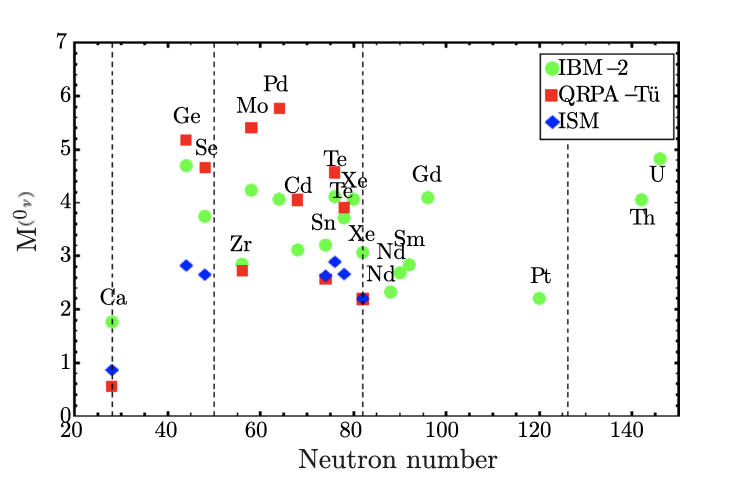
\includegraphics[scale=0.4]{Grafici/NME.png}
	\caption{I valori dei NMEs in funzione del numero di neutroni calcolati secondo i modelli IBM-2~\cite{barea:prc13}, QRPA-T\"{u}~\cite{simkovic:prc13} e ISM~\cite{menendez:npa08}. Figura tratta da~\cite{barea:prc15}.} \label{fig:NME}
\end{figure}



\section{\iflanguage{italian}{Reazioni di DCE e \doppiobeta}{DCE reactions and \doppiobeta}}


%In questo scenario appare evidente la necessità di dedurre dai dati sperimentali nuove informazioni, così da imporre limiti più stringenti ai modelli.  
Da quanto appena detto appare evidente la necessità di imporre limiti più stringenti ai modelli teorici, deducendo dai dati sperimentali nuove informazioni. 
%infatti, nonostante i NMEs non siano direttamente misurabili, sotto opportune condizioni e grazie a modelli teorici appropriati è possibile desumerne il valore tramite misure sperimentali di sezioni d'urto assolute.
In questa prospettiva, le reazioni di \emph{doppio scambio di carica} (Double Charge Exchange, DCE), ovvero le reazioni in cui la carica nucleare cambia di due unità lasciando invariato il numero di massa, si configurano come un potente strumento d'indagine sul \doppiobeta; 
%A causa della bassa sezione d'urto di tali processi, al fine di identificare le reazioni di DCE è essenziale la misura gli spettri energetici con grande risoluzione e le sezioni d'urto assolute ad angoli prossimi a zero.
infatti, sebbene i due processi siano mediati da interazioni differenti, ci sono diverse importanti similarità fra loro.
In primo luogo, gli stati nucleari iniziali e finali del DCE coincidono con quelli del \doppiobeta{}, in quanto in entrambi i casi avviene la trasformazione di due neutroni (protoni) in due protoni (neutroni). 
Un'altra significativa somiglianza riguarda gli operatori di transizione, i quali in tutte e due i processi contengono le componenti a corto range di Fermi, Gamow-Teller e tensoriale di rango-2, con un peso relativo che nelle reazioni di DCE dipende dall'energia incidente. 
Inoltre, in entrambi i casi nel canale intermedio virtuale l'impulso lineare è molto grande, dell'ordine di 100~MeV/c~\cite{barea:prl12}. Questo è un aspetto cruciale, poiché significa che sia le reazioni di DCE sia il \doppiobeta{} sondano stati ad alto impulso della funzione d'onda nucleare, mentre altri meccanismi non ne sono in grado~\cite{puppe:prc11}.

Le reazioni di DCE possono essere uno strumento utile per la comprensione del \doppiobeta{} in quanto permettono di studiare un fenomeno estremamente raro attraverso un meccanismo che, essendo guidato dall'interazione forte, possiede dei tempi caratteristici molto più brevi. 
In aggiunta, il processo di DCE ha il vantaggio di poter essere studiato attraverso misure sperimentali in un laboratorio, in una condizione che consente di tenere sotto controllo alcuni dei parametri fondamentali.
Tuttavia, l'analisi delle reazioni di DCE presenta anche degli inconvenienti: in primis, tali reazioni sono caratterizzate da sezioni d'urto molto basse, tipicamente di alcune decine di nb.
Di conseguenza, per accumulare una statistica sufficiente possono essere necessari lunghi tempi di raccolta dei dati e, a seconda dell'isotopo studiato, fasci di intensità molto grande.
Inoltre, al fine di identificare le reazioni di interesse è essenziale misurare con grande risoluzione e accuratezza sia gli spettri energetici sia le sezioni d'urto assolute ad angoli prossimi a zero. 
%Inoltre, risulta necessario misurare anche gli altri canali di reazione, in modo da  identificare e quantificare i processi di transfer di nucleoni multi-step che concorrono al meccanismo diretto. Questi contributi possono essere minimizzati grazie ad una scelta opportuna del sistema proiettile-target e dell'energia incidente.
Infine, non bisogna dimenticare che eventi così rari sono sommersi da un grande fondo; risulta, dunque, necessario misurare anche gli altri canali di reazione, in modo da poter identificare e quantificare i processi di transfer di nucleoni multi-step che competono con il meccanismo diretto.




\section{\iflanguage{italian}{Il progetto NUMEN}{The NUMEN project}} \label{sez:progetto_numen}

Il progetto NUMEN propone un nuovo metodo per estrarre informazioni basate sui dati sperimentali sui NMEs che entrano in gioco nel calcolo del tasso di dimezzamento del \doppiobeta{}. 
%utilizzando misure accurate di sezioni d'urto di reazioni di DCE indotte da ioni pesanti. 
Per raggiungere tale scopo si intende misurare con grande accuratezza le sezioni d'urto di reazioni di DCE indotte da ioni pesanti, esplorando a diverse energie del fascio incidente \emph{tutti} gli isotopi coinvolti negli esperimenti presenti e futuri sul \doppiobeta{}.
%In particolare, è importante verificare se le sezioni d'urto misurate del DCE sono legate ai NMEs del \doppiobeta{} come una funzione lentamente variabile dell'energia del proiettile e della massa del sistema.%cioè tipo $M^{DCE} \propto f(E_p, A, M^{0 \nu})$
%In tal caso, sarebbe possibile accedere agli elementi di matrice del \doppiobeta{} tramite misure di sezioni d'urto sperimentali. Dal punto di vista teorico, è necessario descrivere accuratamente il meccanismo di reazione, che deve essere fattorizzato in una parte di reazione ed una di struttura nucleare, con quest'ultima a sua volta fattorizzata nel termine del proiettile e in quello del bersaglio.

Il principale, e più ambizioso, obiettivo di NUMEN è l'accesso ai NMEs del \doppiobeta{} attraverso un approccio sperimentale. A tal fine bisogna verificare se gli elementi di matrice del DCE sono legati ai NMEs del \doppiobeta{} come una funzione lentamente variabile dell'energia del proiettile e della massa del sistema.
Qualora questa ipotesi fosse verificata, sarebbe allora possibile dedurre i NMEs del \doppiobeta{} a partire da misure di sezioni d'urto.
% ******* Prima avevo scritto questo:
%Se i risultati sperimentali confermassero che gli elementi di matrice del DCE sono legate ai NMEs del \doppiobeta{} come una funzione lentamente variabile dell'energia del proiettile e della massa del sistema, allora sarebbe possibile dedurre questi ultimi a partire da misure di sezioni d'urto. 
Ciò richiede che il meccanismo di reazione possa essere descritto come il prodotto di un fattore dovuto alla mera reazione e di uno relativo alla struttura nucleare, con quest'ultimo a sua volta fattorizzato in un termine del proiettile e in uno del bersaglio.
%Tale approccio si è dimostrato valido nel caso delle reazioni di singolo scambio di carica (vv. articolo Taddeucci 1987). 
Lo sviluppo di una teoria microscopica coerente della reazione di DCE è, dunque, parte indispensabile del progetto. 
Dal punto di vista sperimentale, la verifica della validità di questa ipotesi richiede la costruzione di una sistematica di dati, che comprenda tutti gli isotopi soggetti al \doppiobeta.
%Sebbene per alcuni casi l'attuale apparato sperimentale possa essere sufficiente, tale studio sistematico richiede l'utilizzo di fasci di intensità molto più elevate di quelle al momento disponibili.
Poiché, come accennato nella sezione precedente, la maggior parte dei processi di DCE presenta sezioni d'urto estremamente basse, tale studio sistematico richiede l'utilizzo di fasci di intensità molto più elevate di quelle al momento disponibili.
In quest'ottica rientra la grande opera di ristrutturazione delle due principali componenti sperimentali: il Ciclotrone Superconduttore (CS) K800 e lo spettrometro magnetico MAGNEX.
%, affrontando le sfide connesse alla ricerca di fenomeni tanto rari, come la bassa sezione d'urto, la grande quantità di background, la necessità di alta risoluzione e sensibilità. 

Altro importante obiettivo di NUMEN consiste nella validazione delle teorie di struttura nucleare che si occupano di calcolare i NMEs del \doppiobeta{};
% ****** Prima avevo scritto:
%; infatti, poiché gli elementi di matrice del DCE e quelli del \doppiobeta{} contengono le stesse funzioni d'onda iniziali e finali e operatori di transizione con struttura simile, la misura di sezioni d'urto assolute può sondare la bontà dei model space adottati dai diversi metodi di calcolo.
infatti, gli elementi di matrice del DCE e quelli del \doppiobeta{} contengono le stesse funzioni d'onda iniziali e finali e operatori di transizione con struttura simile. Se scegliendo un determinato modello di struttura nucleare (con i relativi troncamenti alla funzione d'onda many-body) si trova un buon accordo con i dati sperimentali sulla sezione d'urto del DCE, allora quello stesso model space deve descrivere bene le funzioni d'onda del \doppiobeta.
% Dalla tesi di Ale: "Validare con i dati sperimentali l’applicazione di certi tagli sullo spazio di modello usato nell’analisi dei dati di DCE serve a validare la scelta dello stesso spazio di modello quando l’operatore non è più quello del doppio scambio di carica ma quello del decadimento 0νββ. In questo senso risulta essenziale avere il pieno controllo sulla componente di reazione della sezione d’urto."
Quindi, una volta scelte queste ultime dal confronto con le sezioni d'urto del DCE, le stesse possono essere impiegate per i NMEs del \doppiobeta{}. 

%Infine, NUMEN potrebbe fornire informazioni sulla sensibilità necessaria per la misura del tempo di dimezzamento del \doppiobeta{} a seconda dell'isotopo utilizzato. 
%Infine, NUMEN potrebbe fornire informazioni importanti sui diversi isotopi utilizzati nella ricerca del \doppiobeta{}, perché, facendo il rapporto delle sezioni d'urto assolute misurate negli esperimenti di DCE, si ottiene una stima di quanto il processo sia probabile indipendentemente dal modello adottato. Questa procedura, che consente di ridurre la presenza di eventuali errori sistematici poiché nel rapporto i due contributi si compensano, potrebbe 
Infine, NUMEN potrebbe fornire informazioni importanti sui diversi isotopi utilizzati nella ricerca del \doppiobeta{}, perché il rapporto delle sezioni d'urto assolute misurate negli esperimenti di DCE offre una stima di quanto il processo sia probabile, indipendentemente dal modello assunto. 
%Questa procedura, che consente di ridurre la presenza di eventuali errori sistematici poiché nel rapporto i due contributi si compensano, potrebbe permettere di confrontare
Questa procedura consente di ridurre la presenza di eventuali errori sistematici poiché nel rapporto i due contributi si compensano.
Tale tipologia di analisi potrebbe avere un grande impatto sui futuri esperimenti sul \doppiobeta{}, in quanto potrebbe dare indicazioni su quale isotopo può essere il miglior candidato alla scoperta del processo e sulla sensibilità necessaria per la sua osservazione. 


Gli ambiziosi obiettivi di NUMEN pongono davanti numerose sfide, che richiedono lo sviluppo e l'utilizzo di tecniche innovative sia nel campo teorico sia in quello sperimentale. 
%In particolare, dal momento che il progetto prevede lo studio di tutti gli isotopi candidati al \doppiobeta{}, è necessario utilizzare fasci di intensità molto più alta di quella attualmente disponibile. 
%In questo contesto si inquadra il previsto upgrade delle infrastrutture dei Laboratori Nazionali del Sud (LNS).
%In particolare, dal momento che per studiare tutti gli isotopi candidati al \doppiobeta{} sono necessari fasci ad alta intensità, è fondamentale lo sviluppo di rivelatori capaci di sostenere un alto rate di conteggi.
%In particolare, dal momento che verranno utilizzati fasci ad alta intensità, per il progetto è fondamentale lo sviluppo di rivelatori capaci di sostenere un alto rate di conteggi; infatti, 
%In particolare, la necessità di utilizzare fasci ad elevata intensità rende di fondamentale importanza lo sviluppo di tecnologie di frontiera nell'ambito dei rivelatori ad alto rate di conteggi.
Fra queste, a causa dell'esigenza di utilizzare fasci ad elevata intensità, sono di fondamentale importanza la ricerca e lo sviluppo (R\&D) di tecnologie di frontiera nell'ambito dei rivelatori ad alto rate di conteggi.
%In questo tipo di attività le simulazioni costituiscono un potente strumento per valutare se le performance di un sistema di rivelazione possono soddisfare ai requisiti necessari, evitando così di dedicare tempo e risorse su soluzioni inefficaci.
In questo tipo di attività le simulazioni costituiscono un potente strumento per valutare se una soluzione può soddisfare ai requisiti necessari.

In questo contesto si colloca il ruolo del presente lavoro di tesi, che ha contribuito all'analisi attraverso simulazioni Monte Carlo delle prestazioni di un sistema di rivelazione a stato solido per l'identificazione di ioni pesanti.
%Al fine di validare i risultati della simulazione, è stata svolta un'analisi dei dati sperimentali raccolti in occasione di un test beam svolto ad Aprile 2018, in cui
%I risultati della simulazione sono stati validati con i dati sperimentali del test beam svolto ad Aprile 2018.
Un importante aspetto del presente lavoro verte sulla validazione dei risultati della simulazione attraverso il confronto con i dati sperimentali del test beam svolto ad Aprile 2018, in cui è stata studiata la risposta di un prototipo del sistema di rivelazione simulato.


%All'interno del progetto NUMEN, il presente lavoro di tesi ha contribuito all'analisi attraverso simulazioni Monte Carlo delle prestazioni di un sistema di rivelazione a stato solido per l'identificazione di ioni pesanti.


%L'attuale sistema di rivelazione, basato su pad di silicio, verrebbe danneggiato da tali intensità, quindi servono rivelatori con robustezza alle radiazioni.
%In particolare, è previsto una profonda trasformazione delle due principali infrastrutture sperimentali dell'intero progetto: il Ciclotrone Superconduttore (CS) K800 e lo spettrometro magnetico MAGNEX. 
%Sebbene per alcuni casi 

%L'upgrade dei lns è parte integrante del progetto.

\section{\iflanguage{italian}{L'upgrade dell'apparato sperimentale}{Upgrade of the experimental set-up}} \label{sez:upgrade_apparato}

Come anticipato nella sezione precedente, al fine di studiare in modo sistematico tutti gli isotopi candidati al \doppiobeta{} è necessario utilizzare fasci di intensità molto più alte di quelle disponibili con l'attuale infrastruttura. Dunque, parte integrante di NUMEN è l'upgrade delle due componenti chiave del progetto, il CS e MAGNEX. 
È previsto che, alla fine del processo di ristrutturazione, l'apparato sperimentale possa essere in grado di lavorare con una corrente aumentata di due o tre ordini di grandezza, passando dalle attuali $10^{11}$~pps a circa $10^{13}$~pps.
%Poiché l'aumento della corrente deve essere di due o tre ordini di grandezza
Questo obiettivo può essere raggiunto soltanto a seguito di importanti cambiamenti nelle tecnologie utilizzate nell'estrazione e nel trasporto del fascio, nella realizzazione dei bersagli e nel sistema di rivelazione degli eiettili. 
In particolare, per quanto riguarda quest'ultimo aspetto, i principali cambiamenti previsti sono:
\begin{itemize}
	\item[--] l'aumento della massima rigidità magnetica accettata;
	\item[--] la sostituzione dell'attuale tracciatore a gas, basato su una tecnologia a fili, con un sistema che utilizza i rivelatori Thick-GEM~\cite{cortesi:rsi17};
	\item[--] la sostituzione dell'attuale muro di rivelatori a pad di silicio con una matrice di rivelatori di più piccola taglia e con migliori proprietà di resistenza alle radiazioni;
	\item[--] lo sviluppo di una matrice di rivelatori attorno al bersaglio per la misurazione dei raggi gamma emessi nella diseccitazione degli stati nucleari popolati nelle reazioni di DCE;
	\item[--] l'utilizzo di una nuova elettronica di front-end e di read-out in grado di gestire l'elevato tasso di eventi e l'alto numero di canali previsto.
\end{itemize}
%Dunque, la necessità di sostenere alti rate di particelle porterà ad un profondo cambiamento dell'attuale rivelatore di piano focale (Focal Plane Detector, FPD) di MAGNEX, descritto nel capitolo successivo (\textcolor{red}{aggiungere la sezione}).
Dunque, al fine di raggiungere gli obiettivi preposti da NUMEN è necessaria una profonda trasformazione dell'attuale rivelatore di piano focale (Focal Plane Detector, FPD) di MAGNEX, descritto nel Paragrafo~\ref{sez:progetto_numen}.


%Dei cambiamenti precedentemente elencati particolare attenzione merita quello del tracciatore a gas 
%È importante sottolineare un aspetto dei cambiamenti precedentemente elencati: la sostituzione dell'attuale tracciatore a gas con un sistema 
Dei cambiamenti precedentemente elencati è importante sottolineare un aspetto: il sistema di tracciamento attuale, oltre a fornire accurate informazioni sulla posizione, è sensibile alla perdita di energia degli ioni nel gas. Esso viene, quindi, utilizzato anche come stadio $\Delta E$ per l'identificazione in numero atomico ($Z$) dei prodotti di reazione.
La tecnologia delle Thick-GEM, scelta perché promette buone proprietà di misura della posizione anche in presenza di alti rate, non è invece in grado di dare informazioni sull'energia persa dagli ioni.
Inoltre, gli attuali rivelatori a larga area al silicio, usati per misurare l'energia residua ($ E_{resid} $), non soltanto verrebbero danneggiati da rate così alti, ma sarebbero anche soggetti ad un significativo pile-up a causa delle loro grandi dimensioni.
Di conseguenza, per non diminuire le attuali capacità complessive di identificazione delle particelle (Particle IDentification, PID) è necessario introdurre nel FPD un sistema dedicato a questo scopo.



\subsection{\iflanguage{italian}{Il nuovo sistema di identificazione delle particelle}{The new system of particle identification}} \label{sez:sistema_identif_part}


Il requisito fondamentale che il nuovo sistema di PID deve soddisfare è l'identificazione degli ioni nella regione dell'ossigeno (O), del fluoro (F) e del neon (Ne). 
Oltre a questo, esso deve possedere le seguenti caratteristiche:
\begin{enumerate}
	\item alta resistenza alle radiazioni, in quanto il flusso complessivo atteso sarà dell'ordine di 10\ap{12} $\mbox{ioni}/(\mbox{cm}^2 \cdot \mbox{anno})$;
	\item la risoluzione energetica deve essere sufficientemente buona da garantire una chiara identificazione dei prodotti di reazione di interesse per NUMEN;
	\item il grado di segmentazione deve essere scelto in modo da mantenere la probabilità di eventi con double-hit inferiore al 3\%;
	\item la frazione di volume attivo deve essere sufficientemente alta da ridurre al minimo il fondo costituito dagli eventi con raccolta di carica parziale;
	\item lo spessore dei rivelatori deve riuscire a fermare gli eiettili di interesse in un grande range di energia di incidenza;
	\item i rivelatori devono essere facilmente costruibili e maneggiabili e avere un costo ragionevole.
\end{enumerate}


Dopo aver valutato diverse opzioni, si è scelto di utilizzare un muro di telescopi $ \Delta E - E $ a stato solido.
Negli esperimenti di fisica nucleare questo genere di sistema è tipicamente composto da uno stadio $\Delta E$ sottile al silicio, seguito da un rivelatore spesso al silicio o da uno scintillatore per fermare lo ione.
%La correlazione tra l'energia persa nel primo stadio e l'energia residua depositata nel secondo è legata al numero atomico dello ione rivelato, in accordo con la nota formula di Bethe-Block\cite{knoll:10}.
%Tale tecnica permette l'identificazione degli ioni poiché la correlazione tra l'energia persa nel primo stadio e l'energia residua depositata nel secondo è legata al numero atomico dello ione rivelato, in accordo con la nota formula di Bethe-Block~\cite{knoll:10}.
Tale tecnica permette l'identificazione degli ioni poiché la correlazione tra l'energia persa nel primo stadio e l'energia cinetica totale è legata al numero atomico dello ione rivelato, in accordo con la nota formula di Bethe-Block~\cite{knoll:10}.

Dal momento che, come già detto in precedenza, i rivelatori al silicio non possiedono le proprietà di resistenza alle radiazioni necessarie per il progetto, la scelta è oggi indirizzata verso un telescopio in cui il primo stadio è costituito da un rivelatore sottile (100~$\mu $m) al carburo di silicio~\cite{tudisco:sensors18} (SiC), mentre il rivelatore di stop è uno scintillatore allo ioduro di cesio (CsI) spesso 1~cm.

%Il principale scopo del presente lavoro di tesi è stato la valutazione 
Al fine di verificare se questa scelta possa garantire le performance di PID e la risoluzione energetica necessarie per gli obiettivi del progetto, è stata implementata una simulazione Monte Carlo sulla piattaforma \geant~\cite{agostinelli:nima02,allison:nima16,allison:ieeetns06}.
Tale simulazione, che costituisce l'argomento centrale del presente lavoro di tesi, ha anche lo scopo di valutare la migliore soluzione in termini di granularità, stimando il numero di eventi con raccolta di carica incompleta.








\section{\iflanguage{italian}{Le fasi del progetto}{The phases of the project}}

Il progetto NUMEN è articolato in quattro fasi, di cui verranno esposti i tratti più importanti. 

La \emph{Fase 1}, già completata, ha dimostrato, grazie all'esperimento pilota \ce{^{40}Ca}(\ce{^{18}O},\ce{^{18}Ne})\ce{^{40}Ar}, che è possibile estrarre informazioni sulle funzioni d'onda nucleari del \doppiobeta{} tramite lo studio di reazioni di DCE.

La \emph{Fase 2}, attualmente in corso, prevede lo svolgimento di una campagna sperimentale su alcuni isotopi di interesse, scelti come compromesso tra la rilevanza di tali isotopi per gli esperimenti sul \doppiobeta{} e le esigenze tecniche. I primi sistemi oggetto di studio sono stati $^{116}\mbox{Cd}\,  - \, ^{116}\mbox{Sn} $ e $^{76}\mbox{Ge}\,  - \, ^{76}\mbox{Se} $, sondati attraverso le reazioni (\ce{^{20}Ne}, \ce{^{20}O}) e (\ce{^{18}O}, \ce{^{18}Ne}) per esplorare il meccanismo di DCE in entrambe le direzioni. Prossimamente verrà effettuato un esperimento sulla reazione \ce{^{48}Ti}(\ce{^{18}O},\ce{^{18}Ne})\ce{^{48}Ca}. 
%Durante questa fase verrà anche ottimizzata la strategia di analisi dei dati.
Della Fase~2 fa parte anche l'attività di R\&D su rivelatori, materiali e tecnologie precedentemente descritta.

La \emph{Fase 3} comprende sia lo smontaggio dell'attuale apparato sperimentale sia l'assemblaggio del nuovo. In questa fase avrà luogo anche l'upgrade del CS e della linea di trasporto. La durata prevista è di 18 - 24 mesi.
%La \emph{Fase 3} è dedicata all'upgrade del CS e di MAGNEX: in questa fase 


La \emph{Fase 4} prevede una serie di campagne sperimentali che, grazie alle acquisite condizioni di alta intensità del fascio, comprenderà tutti gli isotopi di interesse per il \doppiobeta{}. 
Questa fase sarà dedicata al calcolo della sezione d'urto assoluta di DCE. Se l'analisi teorica sarà riuscita a sviluppare una descrizione microscopica delle reazioni di DCE, allora sarà possibile avere accesso ai NMEs del \doppiobeta{}, principale obiettivo di NUMEN.










\clearpage


\chapter{\iflanguage{italian}{L'apparato sperimentale}{Experimental set-up}} \label{cap:apparato_sperimentale}


%L'apparato sperimentale attualmente in uso ai LNS-INFN nell'ambito della Fase~2 del progetto NUMEN, costituito principalmente dallo spettrometro MAGNEX e dal Ciclotrone Superconduttore K800, viene brevemente illustrato nella prima parte di questo capitolo.
L'apparato sperimentale attualmente in uso ai LNS-INFN nell'ambito della Fase~2 del progetto NUMEN è costituito principalmente dallo spettrometro MAGNEX e dal Ciclotrone Superconduttore (CS).
Poiché la descrizione di tale apparato non costituisce l'argomento primario di questo lavoro di tesi, nella parte iniziale del capitolo vengono discusse soltanto le sue caratteristiche principali, rimandando alla vasta letteratura sul tema per informazioni più dettagliate (ad esempio~\cite{cavallaro:epja12, carbone:epja12, cappuzzello:epja16, cunsolo:epjst07}).

%Nella prima parte di questo capitolo vengono illustrate le principali caratteristiche dell'apparato sperimentale attualmente in uso ai LNS-INFN nell'ambito della Fase~2 del progetto NUMEN.
%Nella seconda parte viene descritta la configurazione dell'apparato adottata in occasione del test sui telescopi SiC-CsI svolto ad Aprile 2019, sottolineando le differenze rispetto a quella consueta.
Nell'ottica della Fase~4, l'intero apparato sperimentale subirà un importante upgrade, che, in particolare, modificherà radicalmente l'attuale sistema di rivelazione.
Nella seconda parte del capitolo viene, dunque, illustrato il progetto del nuovo Focal Plane Detector (FPD), soffermandosi sulla descrizione dei rivelatori che costituiranno i telescopi SiC-CsI del futuro muro dedicato alla~PID.

%Infine, nella terza parte vengono descritti i due prototipi di telescopio SiC-CsI, su cui ad Aprile~2019 è stato svolto un importante test al fine di verificare

Infine, nella terza parte vengono presentate le condizioni sperimentali in cui è stato svolto il test beam di Aprile~2019, il quale aveva l'obiettivo di valutare le prestazioni dei primi due prototipi di telescopio SiC-CsI e contestualmente verificare la risposta del primo esemplare di elettronica di front-end per il progetto NUMEN.

%del test sui telescopi SiC-CsI svolto ad Aprile~2019, esponendone le motivazioni, descrivendo la configurazione dell'apparato adottata e sottolineandone le differenze rispetto a quella consueta.

%\vspace{0.5 cm}

\section{\iflanguage{italian}{Lo spettrometro magnetico MAGNEX}{MAGNEX magnetic spectrometer}}

Lo spettrometro magnetico MAGNEX è un dispositivo ottico a grande accettanza, costituito da un quadrupolo per la focalizzazione sull'asse verticale, seguito da un dipolo per la dispersione sul piano orizzontale.
Grazie alle sue peculiarità,  MAGNEX riesce ad offrire, in un angolo solido molto grande e in un ampio range energetico, un'ottima risoluzione in energia, angolo e massa.
Ciò lo rende uno strumento ideale per l'analisi di eventi caratterizzati da sezioni d'urto molto basse, come è già stato dimostrato in~\cite{cappuzzello:epja16,pereira:plb12,oliveira:jpg13}.
Inoltre, esso consente di effettuare misure fino a zero gradi, comprendendo, dunque, la regione angolare di massimo interesse per lo studio del DCE.
In Figura~\ref{fig:magnex} è mostrata una foto dello spettrometro, in cui è possibile notare, andando da sinistra verso destra, la camera di scattering, il quadrupolo, il dipolo e il~FPD.


\begin{figure} [!t]
	\centering
	\includegraphics[width=\textwidth, keepaspectratio]{Grafici/magnex_etichette.png}
	\caption{Lo spettrometro magnetico MAGNEX.} \label{fig:magnex}
\end{figure}


La caratteristica che rende MAGNEX uno strumento unico è l'implementazione di una innovativa tecnica di ricostruzione delle traiettorie degli ioni, che consente di correggere le inevitabili aberrazioni originate dalla grande accettanza del dispositivo.
Dunque, a differenza di altri spettrometri magnetici, per MAGNEX è importante determinare non soltanto il punto di impatto sul piano focale ma anche la traiettoria completa. Ciò significa che è necessario misurare quattro parametri: una coppia, chiamata $(x_{foc}, y_{foc})$, individua il punto di impatto sul piano focale, l'altra, indicata con $(\theta_{foc}, \phi_{foc})$, si riferisce rispettivamente all'angolo orizzontale e a quello verticale della traccia al piano focale.
%Nel paragrafo successivo verrà esplicato in che modo vengono misurati tali parametri.
Il modo in cui tali grandezze vengono misurate sarà esplicato nel paragrafo successivo.
%Fra i quattro parametri al piano focale e i 
%
%
%Noti i quattro parametri al piano focale, si procede all'inversione dell'operatore $G$ che esprime il legame fra questi e i quattro parametri sul target.
%Se l'operatore $G^{-1}$ esiste, 
%
Noti i quattro parametri al piano focale, essi vengono utilizzati per risolvere le equazioni del moto di ogni singolo ione e da queste si ricavano i valori delle sezioni d'urto e delle altre quantità di interesse. 




%\clearpage 

%\vspace{0.5 cm}

\subsection{\iflanguage{italian}{L'attuale rivelatore di piano focale}{The present Focal Plane Detector}} \label{sez:fpd}

\begin{figure} [!p]
	\centering
	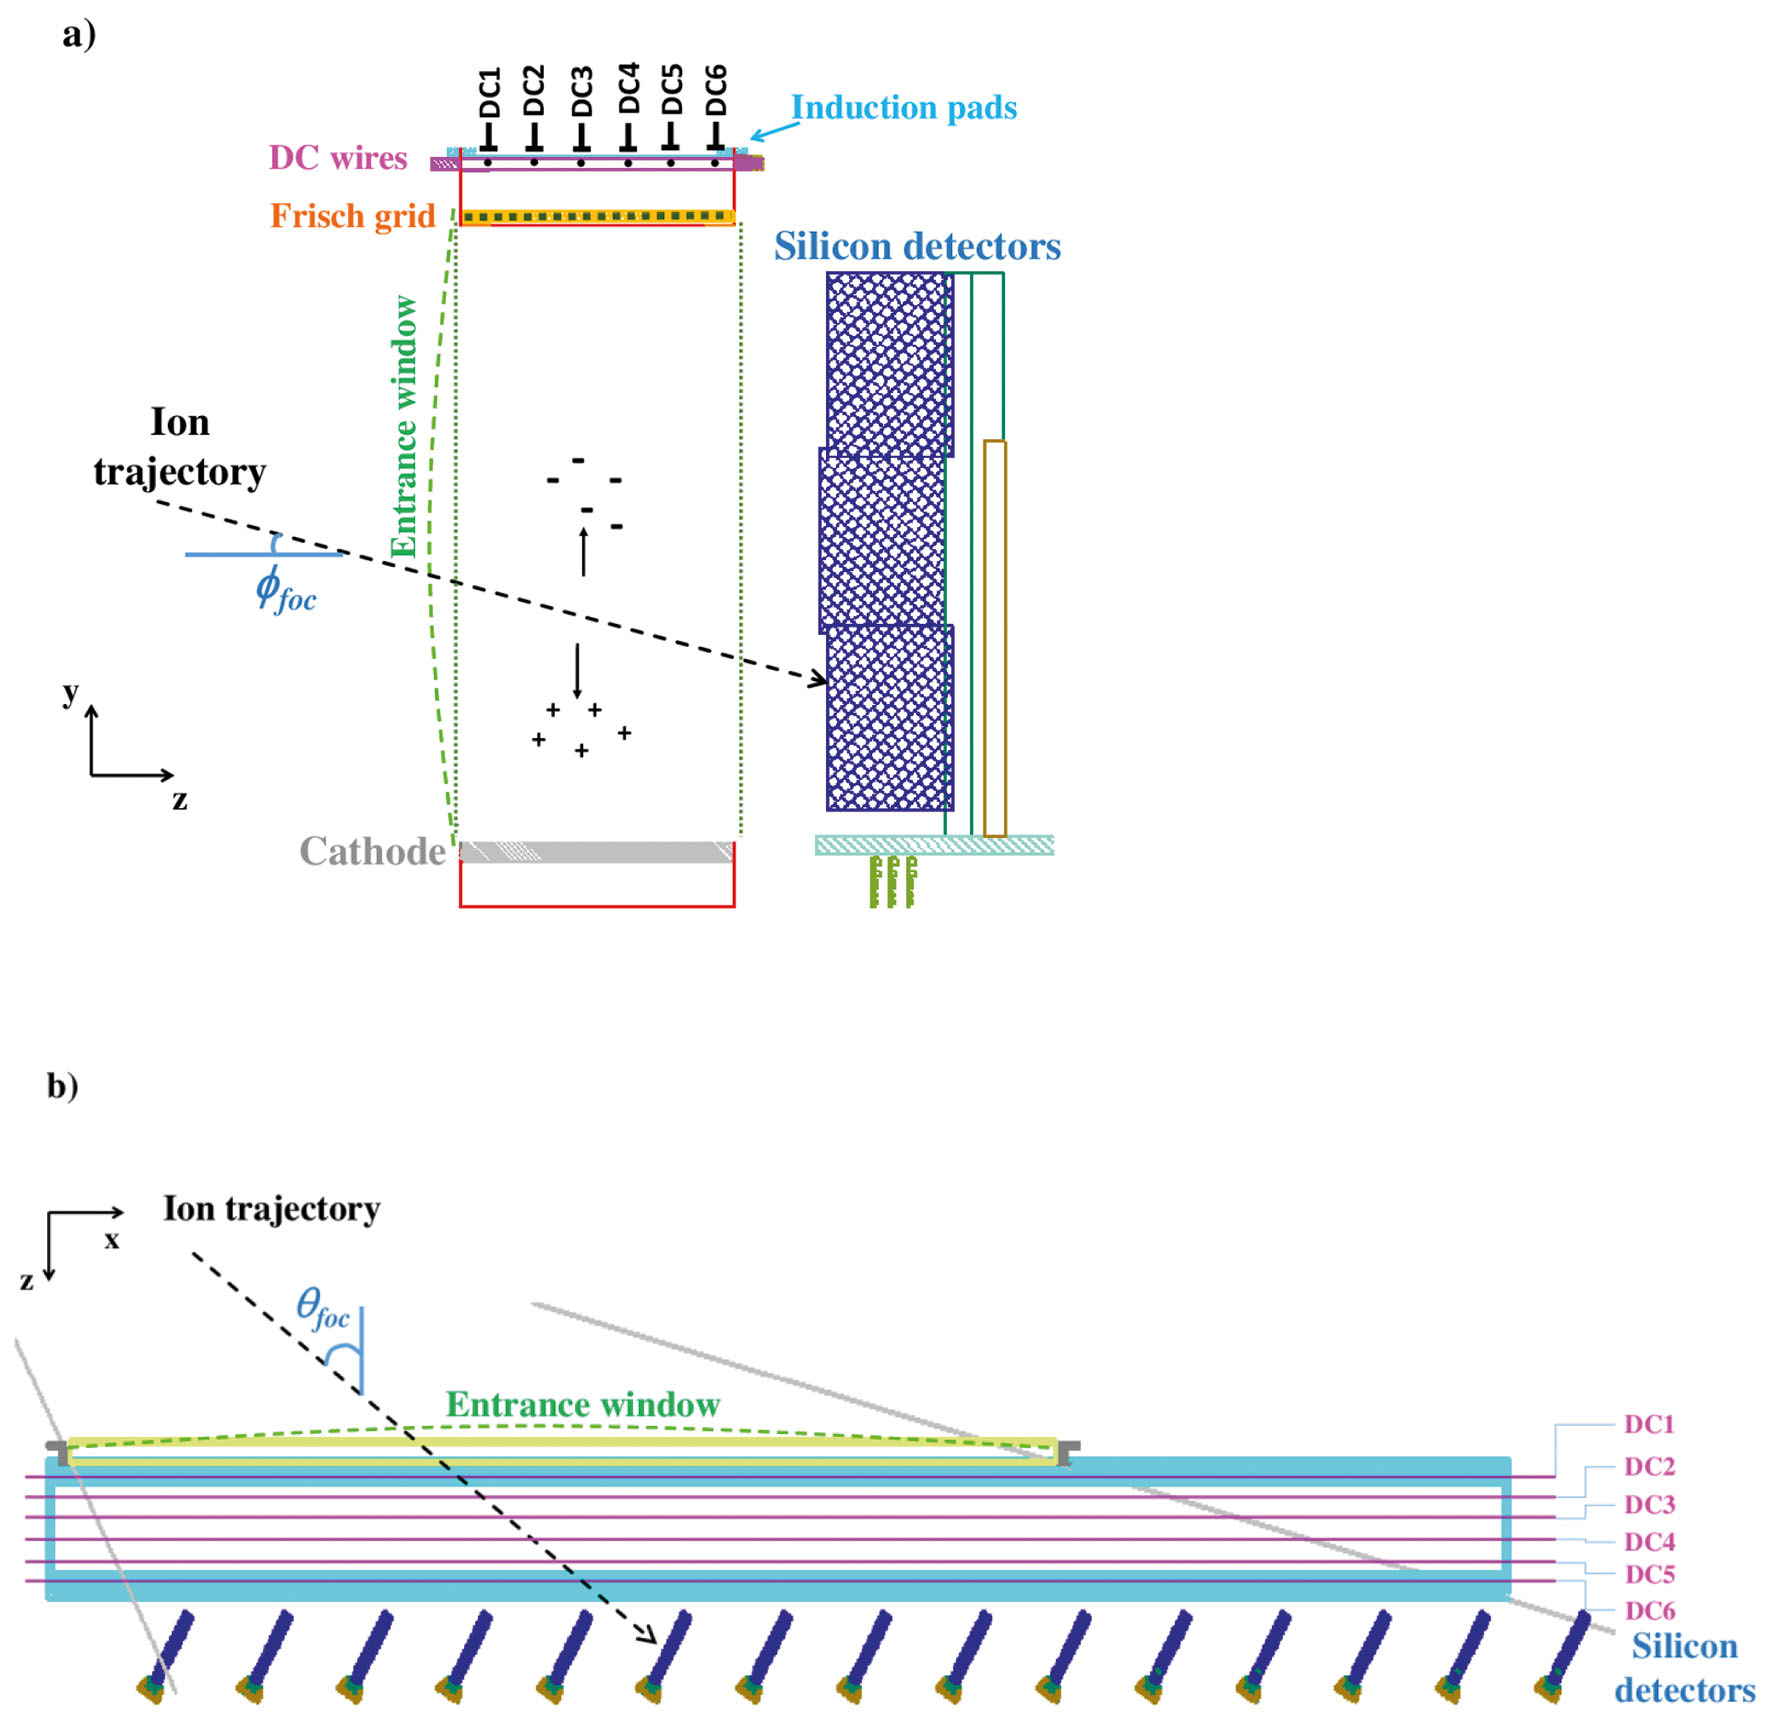
\includegraphics[width=\textwidth, keepaspectratio]{Grafici/fpd.png}
	\caption{Rappresentazione schematica del FPD: a) vista laterale; b) vista dall'alto. Figura tratta da~\cite{cappuzzello:epja18}.} \label{fig:fpd}
\end{figure}


L'attuale FPD di MAGNEX, la cui rappresentazione schematica è riportata in Figura~\ref{fig:fpd}, è un sistema di rivelazione ibrido, costituito da un tracciatore a gas a bassa pressione e da un muro di rivelatori al silicio.
Esso è posizionato a 1.91~m dall'uscita del dipolo e, al fine di minimizzare gli effetti dovuti alle aberrazioni cromatiche~\cite{cunsolo:nima01}, è inclinato di 59.2\textdegree{} rispetto ad un piano perpendicolare all'asse ottico.
%Una finestra di mylar spessa 1.5~$\mu$m è utilizzata per contenere il gas, solitamente costituito da N35 isobutano, segnando l'ingresso nel volume attivo.
L'ingresso nel volume attivo è definito da una finestra di Mylar spessa 2.5~$\mu$m, la quale è utilizzata per contenere il gas, solitamente costituito da N35 isobutano (C\ped{4}H\ped{10}) a pressioni di poche decine di~mbar.



%Il tracciatore a gas è formato da un sistema di sei fili al tungsteno placcati in oro, posti al di sotto di un anodo segmentato in pad. 
%Il tracciatore a gas lavora secondo il principio tipico delle camera a deriva.
%Il tracciatore a gas è essenzialmente una camera a deriva, in cui un sistema misto di fili e pad consente la misura dei quattro parametri necessari.
%Il tracciatore a gas, che consente la ricostruzione tridimensionale della traiettoria degli ioni, è formato da sei fili al tungsteno, indicati con DC\ped{\textit{i}}, e da un anodo segmentato in pad. 
%Al di sopra di ciascun filo si trova una fila di 224 pad
%Il tracciatore a gas è essenzialmente una camera a deriva, in cui un sistema costituito da sei fili (DC\ped{\textit{i}}) e da un anodo segmentato in pad consente la misura dei quattro parametri necessari per la ricostruzione tridimensionale della traccia.
%In particolare, al di sopra di ciascun filo è presente una fila di pad, le quali sono orientate parallelamente all'asse ottico.
Il tracciatore a gas, che consente la ricostruzione tridimensionale della traiettoria degli ioni, è formato da sei fili proporzionali (DC\ped{\textit{i}}) e da un anodo segmentato in sei file di pad, disposte in maniera che sopra ogni filo ci sia una fila di pad.
%Come descritto più avanti, i fili, sfruttando il principio di lavoro delle camere a deriva, danno una misura di sei posizioni verticali ($Y_i$), mentre le pad permettono di determinare sei posizioni orizzontali ($X_i$).
%Una griglia di Frisch è posta al di sotto dei fili, in quanto questi vengono anche utilizzati per misurare l'energia persa dagli ioni nel gas.
%Dal momento che i fili vengono anche utilizzati per misurare l'energia persa dagli ioni nel gas, una griglia di Frisch è posta al di sotto di essi, in modo da rendere il segnale indipendente dalla posizione dell'evento di ionizzazione.




Il muro di rivelatori al silicio, posto all'uscita del tracciatore, è formato da 60 rivelatori, organizzati in 20 colonne da 3 elementi ciascuna. 
%Ogni rivelatore, che ha un'area attiva di $70 \times 50$~mm\ap{2} ed uno spessore di 500~$\mu$m, è montato perpendicolarmente all'asse ottico.
Ogni rivelatore ha un'area attiva di $70 \times 50$~mm\ap{2} ed uno spessore di 500~$\mu$m.
%Ogni pad ha un'area attiva di $70 \times 50$~mm\ap{2} ed è spessa 500~$\mu$m, sufficienti per fermare i prodotti di reazioni nel range energetico di interesse. 
Essi vengono utilizzati per fermare gli ioni, misurandone l'energia residua e producendo il segnale di trigger per l'acquisizione. 

Quando una particella carica, attraversando la finestra di Mylar, entra nel volume attivo, perde energia nel gas producendo coppie elettrone-ione, le quali, sotto l'effetto di un campo elettrico uniforme, migrano rispettivamente verso la griglia di Frisch e il catodo. 
%mentre gli elettroni diffondono verso la griglia di Frisch, con una velocità che per questi ultimi è di circa $3 - 5 $~cm/$\mu$s. 
%La presenza di un campo elettrico costante provoca 
%La velocità di deriva tipica degli elettroni è di $3 - 5 $~cm/$\mu$s
Dopo aver attraversato la griglia, gli elettroni giungono in prossimità dei fili DC\ped{\textit{i}}, dove, a causa dell'elevato campo elettrico, danno luogo alla moltiplicazione a valanga. 
%La carica prodotta, proporzionale all'energia persa dalla particella nel gas, induce sulle pad una distribuzione di carica, della quale si calcola il baricentro. Questa operazione avviene per le sei file di pad, in modo tale che ai sei baricentri corrispondono sei misure di posizioni orizzantali $X_i$.
Alle tensioni e pressioni utilizzate, la carica secondaria prodotta genera un segnale proporzionale all'energia persa dalla particella nel gas. 
Poiché ciò avviene per ciascuno dei sei fili, si hanno sei segnali di perdita di energia, indicati con~$\Delta E_i$.





La stessa valanga induce sulle pad una distribuzione di carica, di cui si calcola il centro di gravità. Anche in questo caso l'operazione si ripete per le sei file di pad, così che vengono estratte sei misure di posizioni orizzontali~$X_i$.
A questo punto, effettuando un fit lineare sulle sei posizioni~$X_i$, si ottengono $x_{foc}$ e $\theta_{foc}$ rispettivamente dall'intercetta e dal coefficiente angolare della retta.

Superata la regione del tracciatore, la particella carica arriva al muro dei rivelatori al silicio, dove si ferma producendo un segnale proporzionale alla sua energia residua~$E_{resid}$. 
Lo stesso segnale viene utilizzato per calcolare l'intervallo di tempo impiegato dagli elettroni primari prodotti nel gas per raggiungere i fili DC\ped{\textit{i}}. 
%Dal momento che tale intervallo è proporzionale allo spazio percorso, si ottengono così sei misure di posizioni verticali~$Y_i$, dalle quali, grazie ad un fit lineare, si ricavano $y_{foc}$ e $\phi_{foc}$ in maniera analoga a quanto visto per $x_{foc}$ e $\theta_{foc}$.
Dal momento che la velocità di deriva è costante, tale intervallo di tempo è direttamente proporzionale allo spazio percorso. Si ottengono, dunque, sei misure di posizioni verticali~$Y_i$, dalle quali, grazie ad un fit lineare, si ricavano $y_{foc}$ e $\phi_{foc}$ in maniera analoga a quanto visto per $x_{foc}$ e $\theta_{foc}$.

È bene ricordare che, nelle camere a deriva a fili, la maggior parte del segnale è originata dal moto degli ioni positivi e non degli elettroni.
Di conseguenza, a causa della minore velocità degli ioni, tale tipologia di rivelatori può tipicamente sostenere rate dell'ordine di pochi~kHz. 
Questo aspetto, che costituisce una delle principali limitazioni all'intensità di fascio tollerabile dall'attuale FPD, deve essere superato nell'ottica della Fase~4. 
%Nasce da qui l'esigenza di sostituire l'attuale tracciatore con un sistema in grado di lavorare con un rate elevato di ioni pesanti. 
%Nasce da qui l'esigenza di sostituire l'attuale
Esso costituisce, dunque, uno dei principali motivi alla base del cambiamento del sistema di rivelazione degli eiettili con uno in grado di lavorare con un rate elevato di ioni pesanti. 
%Da qui trae origine la grande opera di cambiamento del sistema di rivelazione degli eiettili con uno in grado di lavorare con un rate elevato di ioni pesanti.

%\vspace{0.5 cm}

\section{\iflanguage{italian}{Il futuro rivelatore di piano focale}{Future Focal Plane Detector}}

%Il FPD previsto per la Fase~4 del progetto NUMEN manterrà una struttura simile a quella attuale, in quanto consisterà di un sistema di tracciamento tridimensionale a gas e di un muro di rivelatori per la PID.


%Il FPD previsto per la Fase~4 del progetto NUMEN consisterà di un tracciatore tridimensionale e di un muro di telescopi $\Delta E - E$.

Il FPD previsto per la Fase~4 del progetto NUMEN, pur mantenendo una struttura simile a quella attuale, dovrà fare uso di tecnologie innovative, molte delle quali sono ancora in fase di sviluppo.
Esso consisterà di un sistema di tracciamento tridimensionale a gas e di un muro di rivelatori per la~PID.


Il nuovo tracciatore, al momento in fase di sviluppo, dovrà garantire la misura ad alta risoluzione dei quattro parametri $ \left(  x_{foc}, y_{foc}, \theta_{foc}, \phi_{foc}  \right)$ necessari per la ricostruzione della traiettoria in condizioni di alti rate di particelle incidenti. 
%Esso sarà fondamentalmente costituito da tre parti: una regione di deriva per gli elettroni prodotti dalla ionizzazione, un elemento per la moltiplicazione degli elettroni e una scheda segmentata di readout.
Esso sarà fondamentalmente costituito da tre parti:
\begin{itemize}
	\item[--] una regione di deriva per gli elettroni prodotti dalla ionizzazione;
	\item[--] un elemento per la moltiplicazione degli elettroni, ovvero un Micro-Pattern Gas Detector (MPGD);
	\item[--] una scheda segmentata di readout.
\end{itemize}

Il suo principio di lavoro è il seguente: una particella carica incidente, dopo aver attraversato la finestra di mylar per il contenimento del gas, produce lungo la sua traiettoria una traccia di coppie elettrone-ione. 
%Il campo elettrico uniforme fra il catodo e l'elemento per la moltiplicazione guida gli elettroni
%Il campo elettrico uniforme fra catodo e anodo guida gli elettroni primari verso l'elemento di moltiplicazione
Sotto l'azione del campo elettrico uniforme presente fra catodo e anodo, gli elettroni primari si muovono con velocità costante nella regione di deriva fino a raggiungere il MPGD.
Analogamente a quanto visto nel Paragrafo~\ref{sez:fpd}, dalla misura del tempo di deriva degli elettroni primari è possibile estrarre l'informazione sulla posizione e sull'angolo verticali.
%Giunti al MPGD, gli elettroni primari danno origine ad una moltiplicazione a valanga, che risulta nella formazione di un jet elettronico. 
In seguito, gli elettroni primari giungono al MPGD, che dovrebbe essere basato sulla tecnologia delle M-THGEM.
Ciascun THGEM è costituito da una pila di fogli di materiale isolante (solitamente kapton) rivestiti su entrambe le facce con uno strato metallico.
I fogli, che possono avere superfici molto grandi, sono tra loro distanti pochi~mm e si trovano immersi nel gas.
Ogni foglio presenta una trama regolare di fori, i quali hanno un diametro di 0.6~mm.
%Una differenza di potenziale è applicata tra le due superfici metalliche, in modo che gli elettroni vengano guidati verso i fori, dove, incontrando un campo elettrico molto intenso, viene prodotta una moltiplicazione a valanga.
Quando gli elettroni arrivano al primo foglio, la differenza di potenziale applicata tra le due superfici metalliche li guida verso i fori, dove, sotto l'effetto di un campo elettrico molto intenso, producono una moltiplicazione a cascata.
A questo punto, la valanga viene indirizzata da un'ulteriore differenza di potenziale verso il foglio successivo, dando luogo ad una seconda moltiplicazione.
Il processo si ripete per i diversi stadi (2 o 3 a seconda del sistema utilizzato) della M-THGEM, fino a raggiungere fattori di guadagno dell'ordine di $10^4 \div 10^5$. 
Superato l'ultimo foglio, la valanga viene guidata dal campo elettrico verso la scheda segmentata di readout, dove induce su delle strip un impulso di carica. 
Di conseguenza, note le strip coinvolte, è possibile misurare la posizione e l'angolo orizzontali. 





Dopo aver attraversato il tracciatore a gas, la particella carica raggiunge il muro per la PID.
%, che, come anticipato nel Paragrafo~\ref{sez:sistema_identif_part}, sarà costituito da una matrice di telescopi $\Delta E - E$ basati sulla tecnologia SiC-CsI.
%Poiché la simulazione svolta per questo lavoro di tesi verte principalmente su tale argomento,
Poiché l'argomento principale del presente lavoro di tesi consiste nella simulazione di tale sistema di identificazione, per maggiore chiarezza si è preferito discuterne le caratteristiche nella sezione successiva.

%La scelta della tecnologia da utilizzare per il MPGD è oggi orientata verso le Thick-GEM, che, grazie alla loro capacità di sostenere rate fino al MHz/mm\ap{2}, sono adatte agli scopi di NUMEN.
Grazie alla loro capacità di sostenere rate fino al MHz/mm\ap{2}, le M-THGEM costituiscono un'ottima soluzione alle esigenze di NUMEN anche per applicazioni a bassa pressione.
%Tuttavia, diverse delle condizioni in cui questo tipo di rivelatori è abitualmente impiegato non sono attuabili per NUMEN. 
%In primo luogo, le Thick-GEM sono tipicamente utilizzate con gas a pressione atmosferica, mentre il FPD opera solitamente a pressioni di alcune decine di mbar.
%Inoltre, esse spesso sono utilizzate per rivelare particelle in condizioni di Minimum Ionizing Particle, mentre gli ioni di interesse per NUMEN saranno ben lontani da tali energie.
%In aggiunta, dal momento che diversi tipi di ioni raggiungono il rivelatore, il tracciatore deve avere ...
%Dunque, sebbene incoraggianti risultati siano stati recentemente ottenuti~\cite{cortesi:rsi17}, questa soluzione richiede un'intensa attività di sviluppo.


\begin{figure} [!p]
	\centering
	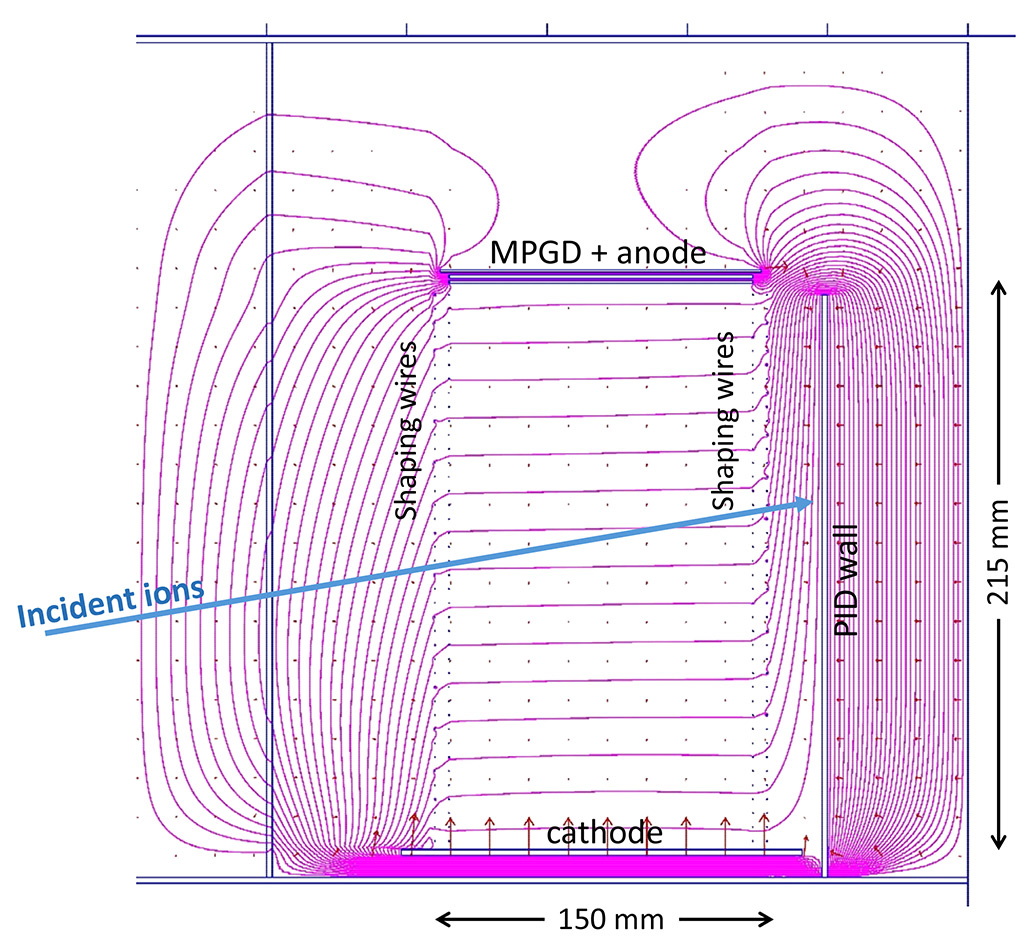
\includegraphics[scale=0.3]{Grafici/nuovo_fpd.png}
	\caption{Rappresentazione schematica del previsto FPD. Le linee magenta indicano le superfici equipotenziali, mentre le frecce mostrano il corrispondente campo elettrico. Figura tratta da~\cite{cappuzzello:epja18}.} \label{fig:nuovo_fpd}
\end{figure}


\begin{figure} [!p]
	\centering
	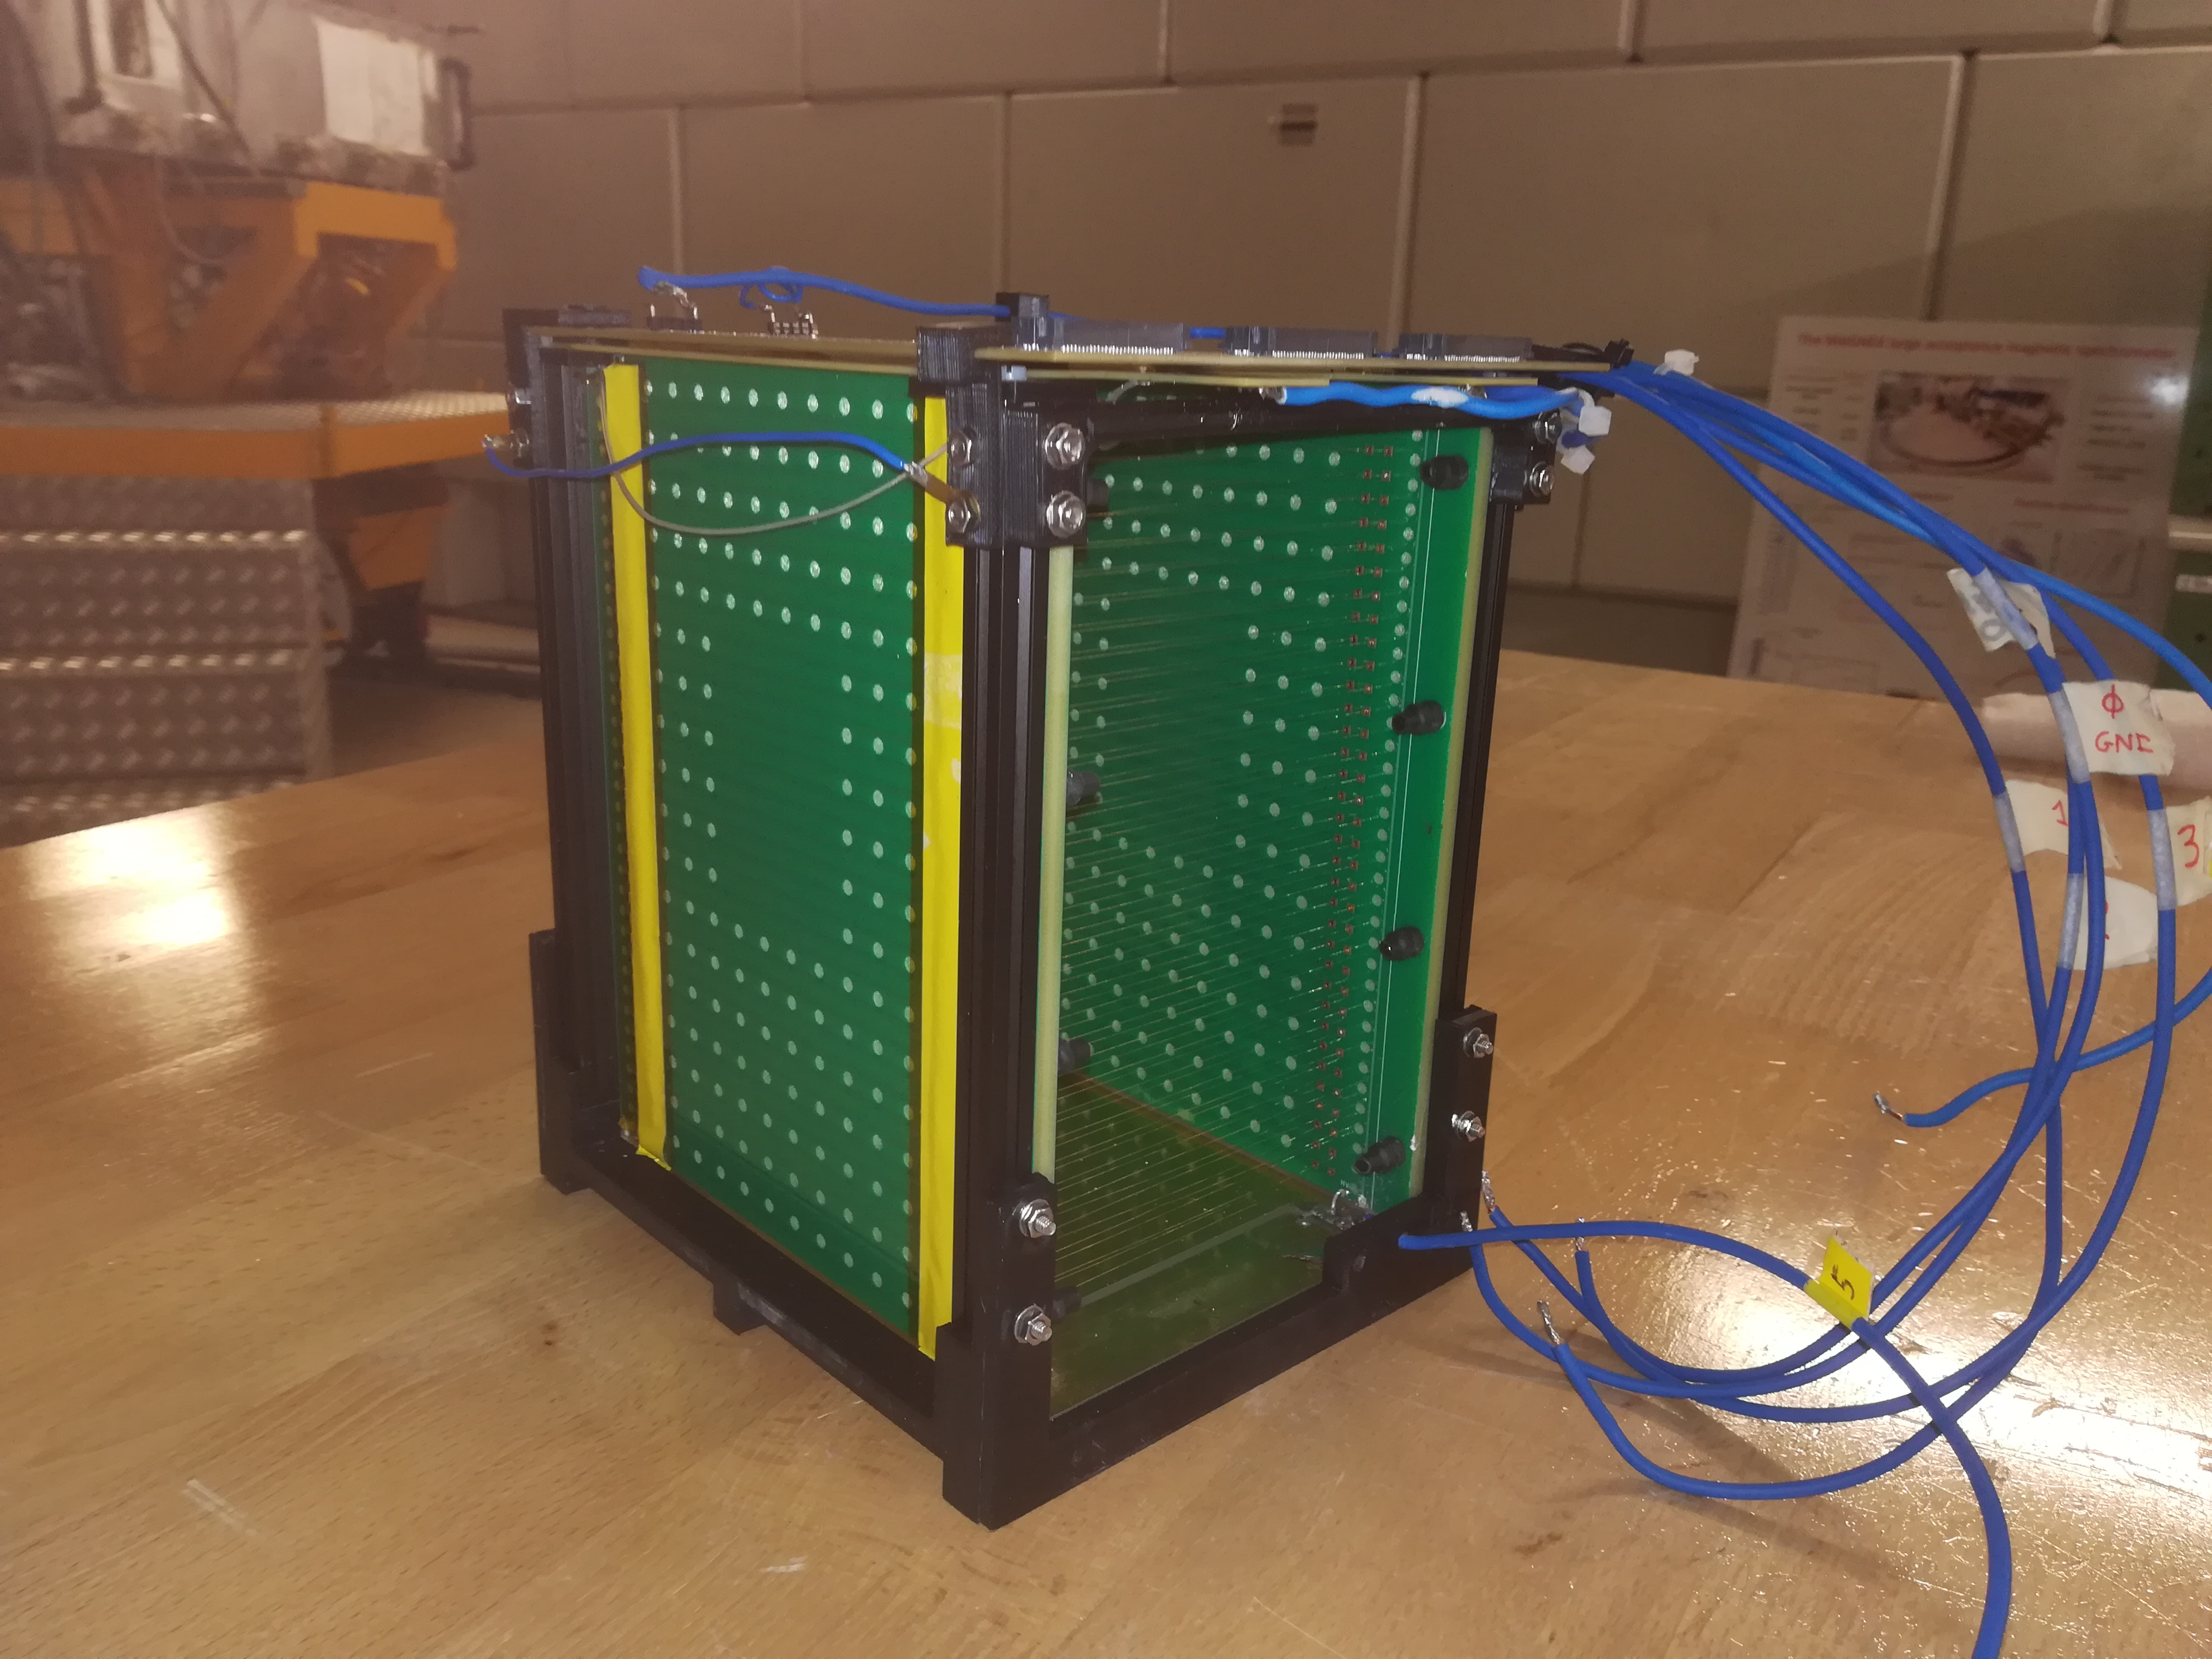
\includegraphics[width=\textwidth, keepaspectratio]{Grafici/castelletto3.jpg}
	\caption{Il prototipo del sistema di tracciamento previsto per NUMEN.} \label{fig:castelletto}
\end{figure}



Una rappresentazione schematica del futuro FPD è mostrata in Figura~\ref{fig:nuovo_fpd}, dove sono raffigurate anche le superfici equipotenziali calcolate con il codice Poisson-Superfish~\cite{superfish:87}: le linee quasi parallele indicano che nella regione di deriva il campo elettrico è piuttosto uniforme.


Un prototipo di dimensioni ridotte, mostrato in Figura~\ref{fig:castelletto}, è stato realizzato per individuare le migliori soluzioni in termini di geometria, tensioni applicate, MPGD ed elettronica.








%\vspace{0.3 cm}

%\clearpage
%\section{\iflanguage{italian}{Il test sui telescopi SiC-CsI}{Experimental setting for the test}}

\section{\iflanguage{italian}{I telescopi SiC-CsI}{SiC-CsI telescope detectors}}

%Ad Aprile 2019 è stato svolto un test sui primi due prototipi di telescopi SiC-CsI, allo scopo di confrontarne la risposta con il sistema attualmente utilizzato.
%Ad Aprile 2019 è stato svolto un test sui primi due prototipi di telescopi SiC-CsI, allo scopo di valutarne la risposta, confrontandola con quella del sistema attualmente utilizzato.


%Dopo aver realizzato 
%Per verificare se la risposta di un telescopio formato da uno stadio $\Delta E$ al SiC seguito da un cristallo di CsI poteva garantire prestazioni di identificazione degli ioni confrontabili con quelle accessibili con l'attuale apparato, è stato svolto un test per una durata complessiva di cinque giorni.
%Dal momento che tali rivelatori non sono ancora uno standard nel mondo della fisica ma rappresentano una tecnologia nuova, è stato svolto un test per verificare se le loro prestazioni possono soddisfare le esigenze di NUMEN.

%Come illustrato nel Paragrafo~\ref{sez:sistema_identif_part}, i rivelatori al SiC sono stati scelti nell'ambito del progetto per assolvere al ruolo di sistema di PID
%Sono stati, dunque, assemblati due telescopi SiC-CsI, di cui si è studiata la risposta in termini di PID.

%Come illustrato nel Paragrafo~\ref{sez:sistema_identif_part}, i rivelatori al SiC sono stati scelti nell'ambito del progetto per identificare i prodotti di reazione

%Quando si studiano le reazioni fra ioni pesanti, l'identificazione in numero atomico, massa e carica dei prodotti di reazione è una componente indispensabile che, a seconda delle esigenze, viene eseguita sfruttando vari metodi.
%Una delle tecniche più diffuse prevede l'utilizzo di telescopi $\Delta E - E$.
Quando si studiano le reazioni fra ioni pesanti, l'identificazione in numero atomico ($Z$), massa ($A$) e carica ($q$) dei prodotti di reazione è una componente indispensabile per la ricostruzione e la misura delle sezioni d'urto.
Il progetto NUMEN, a tale scopo, propone l'utilizzo combinato di diversi metodi: l'identificazione in $Z$ verrà svolta mediante la tecnica $\Delta E - E_{resid}$, mentre per quella in $A$ e $q$ si utilizzeranno anche la deflessione dovuta alla forza di Lorentz e il tempo di volo degli ioni.
%Come anticipato nel Paragrafo~\ref{sez:sistema_identif_part}, il progetto NUMEN ha individuato come possibile soluzione per la PID in condizioni di alti rate di particelle incidenti l'utilizzo di telescopi $\Delta E - E$, in cui il primo stadio è costituito da un rivelatore al carburo di silicio (SiC), mentre il secondo è uno scintillatore allo CsI.
In particolare, come anticipato nel Paragrafo~\ref{sez:sistema_identif_part}, i telescopi $\Delta E - E_{resid}$ saranno costituiti da un primo stadio basato su un rivelatore al carburo di silicio (SiC), seguito da uno scintillatore allo ioduro di cesio (CsI).
Il progetto al momento prevede la realizzazione di un muro composto da 1230 telescopi, arrangiati in 41 colonne.
Ogni colonna è, a sua volta, costituita da 3 moduli contenenti una matrice di $2 \times 5$ telescopi ciascuno.
In Figura~\ref{fig:muro_telescopi} è riportato uno schema di come dovrebbe apparire il futuro muro per la PID.

Prima di proseguire, vediamo più in dettaglio le principali caratteristiche dei rivelatori al SiC e degli scintillatori allo CsI, sottolineando gli aspetti che  hanno guidato verso la loro scelta nell'ambito di NUMEN.


\begin{figure} [!t]
	\centering
	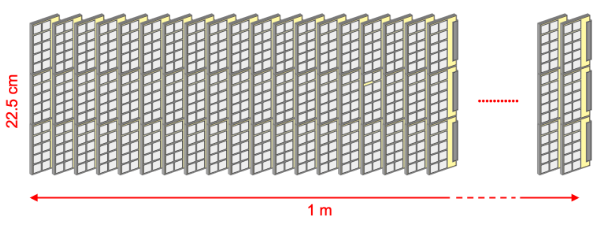
\includegraphics[width=\textwidth, keepaspectratio]{Grafici/muro_telescopi.png}
	\caption{Schema del muro di telescopi previsto per NUMEN.} \label{fig:muro_telescopi}
\end{figure}



%Il fascio utilizzato nel test era costituito da \ce{^{20}Ne}, mentre i bersagli erano \ce{^{197}Au} e \ce{^{12}C}




%\vspace{0.5 cm}
%\clearpage

%\subsection{\iflanguage{italian}{I telescopi SiC-CsI}{SiC-CsI telescope detectors}}

\subsection{\iflanguage{italian}{I rivelatori al carburo di silicio}{Silicon carbide detectors}}


%I dispositivi al SiC costituiscono oggi una promettente realtà nel campo dei rivelatori per la fisica, 
Grazie alle sue interessanti proprietà, il SiC costituisce oggi una promettente realtà nel campo della realizzazione di rivelatori per la fisica, configurandosi come una potenziale alternativa al silicio nelle applicazioni che richiedono una grande resistenza alle radiazioni.
%La larghezza della sua gap, quasi tripla rispetto a quella del silicio, se da un lato aumenta l'energia media per la produzione di una coppia elettrone-lacuna, dall'altro riduce il numero di portatori di carica generati per agitazione termica, mantenendo, dunque, un ottimo rapporto segnale-rumore.
%
%La larghezza della sua gap, quasi tripla rispetto a quella del silicio, se da un lato riduce il numero di portatori di carica generati per agitazione termica, dall'altro aumenta l'energia media per la produzione di una coppia elettrone-lacuna. 
%La larghezza della sua gap, essendo quasi tripla rispetto a quella del silicio, aumenta l'energia media per la produzione di una coppia elettrone-lacuna.
%Esso fa parte dei semiconduttori a grande larghezza di banda
%Dal momento che la larghezza della sua gap è quasi tripla rispetto a quella del silicio, l'energia media per la produzione di una coppia elettrone-lacuna nel SiC è maggiore di quella nel silicio. 
La caratteristica che ha suscitato grande interesse nella comunità scientifica nei confronti di questo materiale deriva dalla larghezza della sua gap, che risulta essere quasi tripla rispetto a quella del silicio.
Ciò implica diverse conseguenze: in primo luogo, dal momento che l'energia media per la produzione di una coppia elettrone-lacuna nel SiC è quasi tre volte quella nel silicio, a parità di energia una particella incidente su un rivelatore al SiC crea un terzo dei portatori di carica prodotti in un rivelatore al silicio.
Dunque, ne deriva un'inferiore ampiezza del segnale generato e, conseguentemente, un peggioramento della risoluzione, in quanto la componente statistica di tale grandezza è inversamente proporzionale alla radice quadrata del numero di portatori~\cite{knoll:10}.
%\textcolor{red}{???} Tuttavia, gli ioni pesanti di interesse per NUMEN, rilasciando molta energia nel rivelatore, producono un numero elevato di portatori, in modo tale che le fluttuazioni statistiche risultano trascurabili.
%
%% MODIFICHIAMO QUESTA PARTE
%Ciò significa che, a parità di energia, una particella incidente su un rivelatore al SiC crea un terzo dei portatori di carica prodotti in un rivelatore al silicio, generando, dunque, un segnale di ampiezza inferiore.
%Ciò significa che, a parità di energia, una particella incidente su un rivelatore al SiC crea un terzo dei portatori di carica prodotti in un rivelatore al silicio.
%
%% PRIMA DELLA CORREZIONE DEL PROF
%Dunque, a parità di energia, una particella incidente su un rivelatore al SiC crea un terzo dei portatori di carica prodotti in un rivelatore al silicio, generando, di conseguenza, un segnale di ampiezza inferiore.
%Ciò ha come conseguenza che il segnale generato presenta un'ampiezza inferiore.
%Ciò ha come effetto un peggioramento della risoluzione, in quanto la componente statistica di tale grandezza è inversamente proporzionale alla radice quadrata del numero di portatori~\cite{knoll:10}.
%Tuttavia, la maggiore larghezza della gap determina una riduzione del numero di coppie generate per agitazione termica, che risulta, dunque, in una diminuzione della corrente inversa e del livello di rumore.
%Tuttavia, la maggiore larghezza della gap determina l'estrema resistenza alle radiazioni del SiC, poiché, sebbene a causa del danno da radiazioni possano introdursi dei livelli in banda proibita, questi possono restare piuttosto lontani dalle bande di conduzione e di valenza.
%Di conseguenza, le transizioni elettroniche da o verso tali livelli possono risultare sfavorite, in modo da non causare un aumento significativo della corrente inversa.
%Tuttavia, la maggiore larghezza della gap determina l'estrema resistenza alle radiazioni del SiC.
%Ciò può essere spiegato nel modo seguente: l'irraggiamento può causare l'introduzione di livelli in banda proibita

%
%% ALTRIMENTI CI METTO QUESTO (Tratto da EPJ)
Tuttavia, la maggiore larghezza della gap del SiC, insieme all'elevata forza dei suoi legami chimici, determina la sua estrema resistenza alle radiazioni.
Tale proprietà può essere spiegata nel modo seguente: quando una particella carica attraversa un rivelatore, oltre a ionizzare ed eccitare gli atomi del mezzo, può causare la comparsa nel reticolo cristallino di interstizi, vacanze o strutture più complesse.
Questi difetti possono introdurre dei livelli nella banda proibita, che alterano le proprietà originali del semiconduttore; in particolare, i principali effetti macroscopici sono: l'aumento della corrente inversa, il cambiamento della tensione di svuotamento e la riduzione dell'efficienza di raccolta di carica, in quanto i difetti agiscono come trappole per i portatori di carica.
Dal momento che il SiC ha una gap piuttosto grande, i livelli nella banda proibita possono comunque risultare piuttosto distanti dalle bande di valenza e di conduzione, in modo tale da sfavorirne il popolamento.
Di conseguenza, sebbene si verifichi la comparsa di tali livelli, la corrente inversa non subisce un aumento significativo.

Inoltre, bisogna ricordare che il danno causato da protoni, neutroni o particelle al MIP è totalmente diverso da quello prodotto da ioni pesanti; infatti, mentre i primi, depositando poca energia nel rivelatore, danno luogo principalmente a fenomeni di dislocamento di singoli atomi, i secondi, rilasciando elevate quantità di energia, possono originare lo spostamento di interi cluster.
Se la prima tipologia di danno può essere contrastata mantenendo i rivelatori a bassa temperatura (come avviene con il silicio), la seconda dipende soltanto dalla resistenza del reticolo.
%Inoltre, l'elevata forza dei legami chimici del SiC si traduce in un'energia di dislocamento di $30 \div 40$~eV, circa tre volte superiore a quella del silicio.
In entrambi i casi il SiC esibisce delle notevoli proprietà di robustezza, in quanto l'elevata forza dei suoi legami chimici si traduce in un'energia di dislocamento di $30 \div 40$~eV, circa tre volte superiore a quella del silicio. 




%Questo ha due diverse conseguenze sul segnale generato: in primis, ne diminuisce l'ampiezza; in secondo luogo, ne aumenta le fluttuazioni relative, in quanto la componente statistica della risoluzione è inversamente proporzionale alla radice quadrata del numero dei portatori~\cite{knoll:10}.
%Se il primo problema può essere risolto aumentando l'amplificazione del segnale, il secondo è intrinseco del rivelatore.
%, dando origine a due diversi problemi: in primo luogo, il segnale generato presenta un'ampiezza inferiore, 
%di conseguenza, 
%di conseguenza, non soltanto il segnale generato presenta un'ampiezza inferiore, ma la risoluzione energetica 
%Di conseguenza, dal momento che la componente statistica della risoluzione è inversamente proporzionale alla radice quadrata del numero dei portatori~\cite{knoll:10}, i rivelatori al SiC hanno una risoluzione  
%
%Dunque, i rivelatori al SiC generano segnali di ampiezza inferiore rispetto a quelli dei rivelatori al silicio.
%
%% CASSIAMO QUESTA PARTE
%Tuttavia, gli ioni pesanti di interesse per NUMEN dovrebbero generare un numero elevato di coppie elettrone-lacuna, così che l'ampiezza del segnale dovrebbe essere sufficientemente grande.
%
%
%Inoltre, i rivelatori al SiC hanno un ottimo rapporto segnale-rumore anche a temperature piuttosto alte, mentre i rivelatori al silicio hanno, in alcuni casi, bisogno di un sistema di raffreddamento.


%Oltre alla resistenza alle radiazioni, un ulteriore vantaggio rispetto ai rivelatori al silicio riguarda il comportamento a temperature piuttosto alte: mentre i rivelatori al SiC continuano ad avere un ottimo rapporto segnale-rumore, i rivelatori al silicio mostrano un aumento della corrente inversa, rendendo a volte necessario l'utilizzo di sistemi di raffreddamento.
Oltre alla resistenza alle radiazioni, i rivelatori al SiC presentano un ulteriore vantaggio rispetto a quelli al silicio: la maggiore larghezza della gap determina una riduzione del numero di coppie generate per agitazione termica, che risulta, dunque, in una diminuzione della corrente inversa e del livello di rumore.
Di conseguenza, anche a temperature piuttosto alte, i rivelatori al SiC continuano ad avere un ottimo rapporto segnale-rumore, mentre i rivelatori al silicio mostrano un aumento della corrente inversa, rendendo a volte necessario l'utilizzo di sistemi di raffreddamento.

Grazie ai notevoli progressi in campo tecnologico, oggi i rivelatori al SiC possono essere realizzati mediante una giunzione p-n, polarizzata inversamente per aumentare l'estensione della regione svuotata e per migliorare l'efficienza di raccolta dei portatori di carica.
Quando una particella carica attraversa il rivelatore, perde energia generando coppie elettrone-lacuna, le quali, in presenza di un campo elettrico, si muovono verso gli elettrodi, producendo un segnale elettrico proporzionale all'energia depositata.

Nella rivelazione di ioni pesanti ad energie maggiori di diverse decine di~MeV (come quelli di interesse per NUMEN), i rivelatori al SiC esibiscono risoluzioni energetiche confrontabili con quelle dei dispositivi al silicio, in quanto viene rilasciata molta energia nel rivelatore e, pertanto, viene prodotto un numero elevato di portatori di carica.
Dunque, le fluttuazioni statistiche sul segnale risultano piccole determinando un trascurabile effetto sulla risoluzione in energia, quest'ultima dominata da altri fattori come il rumore termico, l'accoppiamento con l'elettronica di front-end, etc.
%Inoltre, recenti test hanno dimostrato che con un rivelatore da 100~$\mu$m di spessore è possibile ottenere una risoluzione energetica dello 0.4\%~FWHM per le particelle $\alpha$ dell'\ce{^{241}Am} a 5486~keV~\cite{tudisco:sensors18}, mentre con i rivelatori al silicio per le stesse particelle si possono raggiungere valori dello 0.2\% FWHM~\cite{steinbauer:nimb94}.

Recentemente, diversi test sono stati condotti su rivelatori al SiC dello stesso tipo di quelli che verranno utilizzati per NUMEN: in uno di questi test sono state messe a confronto le prestazioni in termini di risoluzione energetica di tale rivelatore con quelle di un rivelatore al silicio~\cite{tudisco:sensors18}.
I risultati, riportati in Figura~\ref{fig:tudisco_spettro}, dimostrano che col rivelatore al SiC è possibile ottenere una risoluzione energetica dello 0.4\%~FWHM per le particelle $\alpha$ dell'\ce{^{241}Am} a 5486~keV, mentre col rivelatore al silicio per le stesse particelle si è raggiunto un valore dello 0.22\%~FWHM.
\begin{figure} [!p]
	\centering
	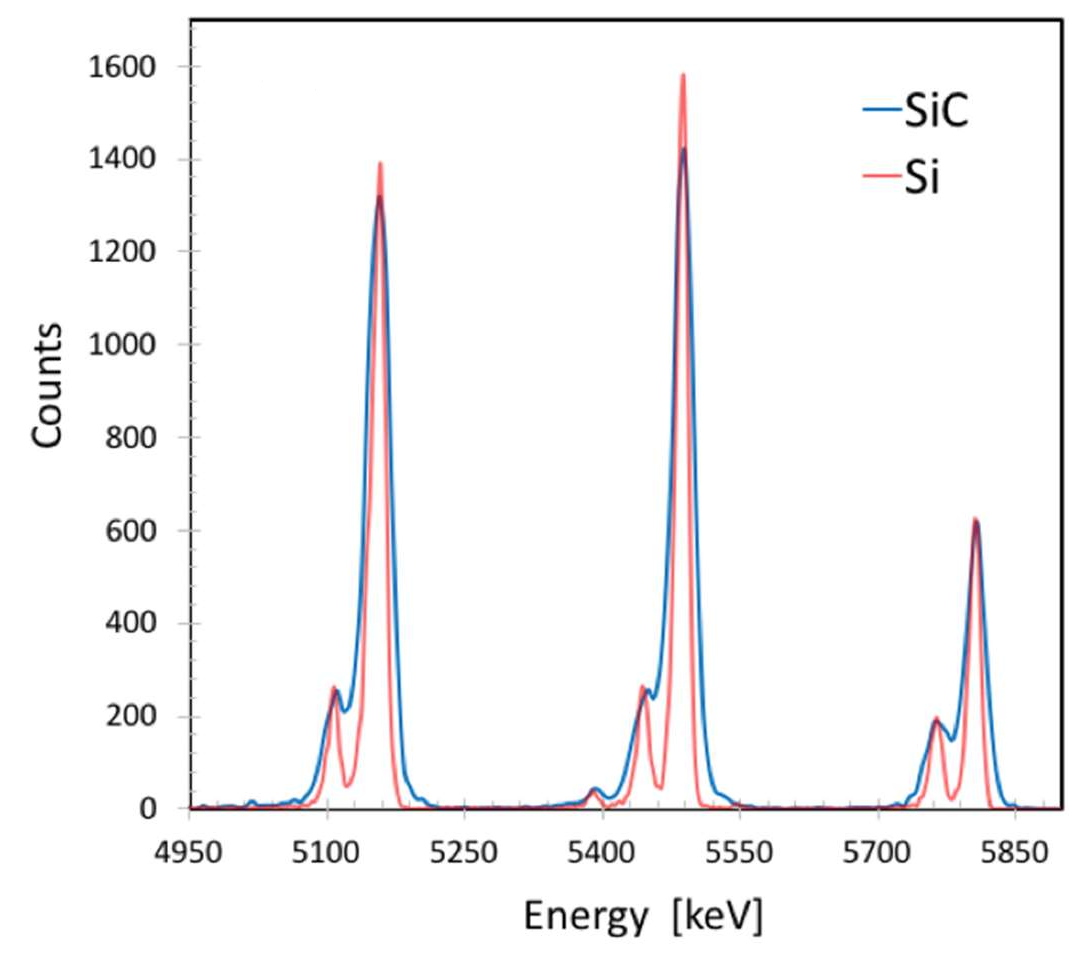
\includegraphics[width=\textwidth, keepaspectratio]{Grafici/spettro_sic_tagliato.png}
	\caption{Spettro energetico della sorgente $\alpha$ (\ce{^{239}Pu}, \ce{^{241}Am}, \ce{^{244}Cm}) misurato da un rivelatore al silicio Hamamatsu S3590 e da un rivelatore al SiC. Figura tratta da~\cite{tudisco:sensors18}.} \label{fig:tudisco_spettro}
\end{figure}
In un altro test~\cite{ciampi:nima19}, il rivelatore al SiC è stato adoperato per la realizzazione di un telescopio SiC-CsI, simile a quelli previsti per NUMEN.
Tale telescopio, la cui rappresentazione schematica è mostrata in Figura~\ref{fig:ciampi_telescopio}, è stato utilizzato per l'identificazione degli eiettili prodotti dalla collisione di un fascio di \ce{^{40}Ca} e \ce{^{48}Ca} a 40~AMeV con un bersaglio di \ce{^{12}C}. 
Le correlazioni $\Delta E - E_{resid}$ sono riportate in Figura~\ref{fig:ciampi_deltaE_E}: come si può notare, i differenti elementi sono ben identificati fino a $Z \sim 20$, consentendo perfino un'identificazione in $A$ per $Z \lesssim 3$.


\begin{figure} [!t]
	\centering
	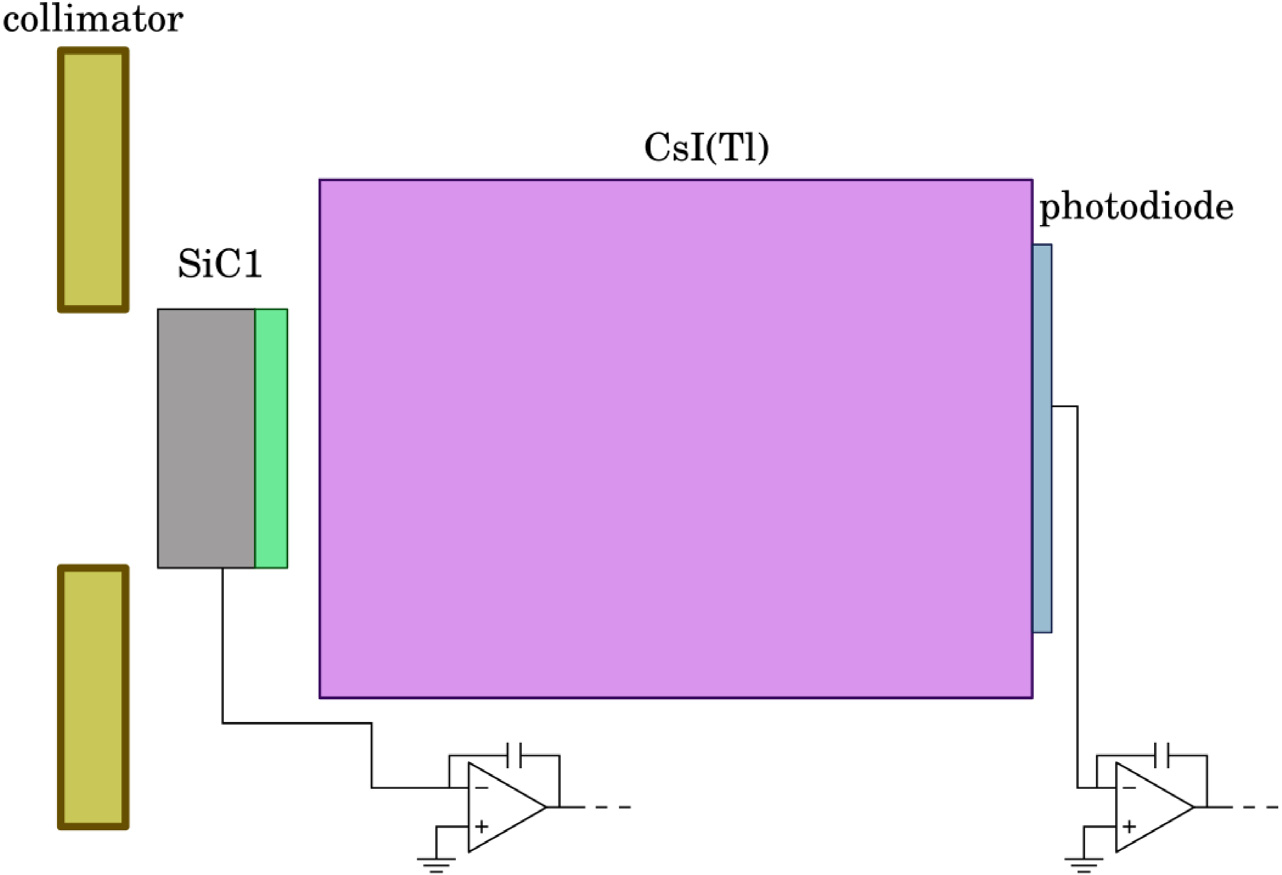
\includegraphics[scale=0.25]{Grafici/ciampi-telescopio.png}
	\caption{Rappresentazione schematica del telescopio SiC-Csi. Per il primo stadio, il substrato (grigio) e l'area sensibile (verde chiaro) sono mostrati in proporzione. Figura tratta da~\cite{ciampi:nima19}.} \label{fig:ciampi_telescopio}
\end{figure}



\begin{figure} [!p]
	\centering
	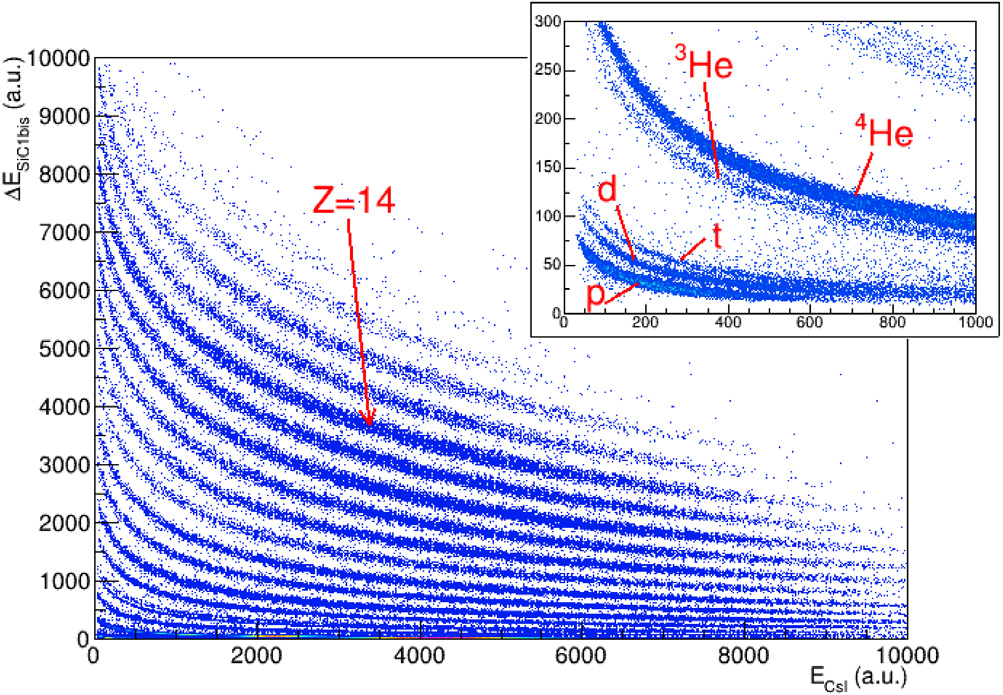
\includegraphics[width=\textwidth, keepaspectratio]{Grafici/ciampi-deltaE-E.png}
	\caption{Le correlazione $\Delta E - E_{resid}$ ottenute con il telescopio SiC-CsI in Figura~\ref{fig:ciampi_telescopio}. Il riquadro nell'angolo in alto a destra mostra uno zoom della regione con $Z \lesssim 2$. Figura tratta da~\cite{ciampi:nima19}.} \label{fig:ciampi_deltaE_E}
\end{figure}

%La resistenza alle radiazioni dei rivelatori al SiC è stata indagata sia attraverso simulazioni Monte Carlo sia per mezzo di test sperimentali. 
%Poiché la resistenza alle radiazioni è l'aspetto di maggiore importanza per la scelta dei dispositivi da utilizzare per NUMEN, alcune simulazioni Monte Carlo sono state implementate allo scopo di darne una stima nel caso dei rivelatori al SiC. 
%In Figura~\ref{fig:sic_simul_resist_radiaz} (a sinistra) sono riportati i risultati della produzione di vacanze generata da protoni e \ce{^{18}O} in un rivelatore da 100~$\mu$m.
%Come si può notare, i difetti causati dagli ioni di ossigeno sono due ordini di grandezza maggiori di quelli indotti dai protoni.
%Un andamento simile si osserva anche per la corrente inversa, mostrata in Figura~\ref{fig:sic_simul_resist_radiaz} (a destra). Sebbene questa aumenti di diversi ordini di grandezza dopo alte dosi di irradiazione, può essere ancora tollerabile, essendo cinque ordini di grandezza inferiore a quella del silicio.

%La resistenza alle radiazioni di rivelatori al SiC di piccole dimensioni ($2 \times 2$~mm\ap{2}, 30~$\mu$m di spessore) è stata analizzata in un test in cui i dispositivi erano irraggiati con ioni pesanti~\cite{raciti:npa10}. 
Dal momento che la resistenza alle radiazioni è un aspetto essenziale per la scelta dei dispositivi da utilizzare per NUMEN, è stata svolta un'attenta ricerca bibliografica per cercare dati sperimentali sul comportamento del SiC quando viene sottoposto ad elevate dosi di radiazioni.
%Da tale ricerca è emerso che su rivelatori di piccole dimensioni ($2 \times 2$~mm\ap{2}, 30~$\mu$m di spessore) è stato condotto un test in cui i dispositivi erano irraggiati con ioni pesanti~\cite{raciti:npa10}.
%Dalla ricerca è emerso che diversi studi sono stati condotti su tale argomento, i quali affermano concordemente che la robustezza del SiC è, a parità di condizioni, molto maggiore di quella del silicio~\cite{garcialopez:nimb16, nava:nima03}; in particolare, è stato realizzato un test su rivelatori di piccole dimensioni ($2 \times 2$~mm\ap{2}, 30~$\mu$m di spessore) in cui i dispositivi erano irraggiati con ioni pesanti~\cite{raciti:npa10}.
%I risultati hanno dimostrato che tali rivelatori sono in grado di sostenere fluenze dell'ordine di $10^{14}$  $\mbox{ioni}/\mbox{cm}^2$.
Dalla ricerca è emerso che diversi studi sono stati condotti su tale argomento, i quali affermano concordemente che la robustezza del SiC è, a parità di condizioni, molto maggiore di quella del silicio~\cite{garcialopez:nimb16, nava:nima03}; in particolare, in un test~\cite{raciti:npa10} si è riscontrato che giunzioni Shottky in SiC possono sostenere fluenze dell'ordine $10^{14}$  $\mbox{ioni}/\mbox{cm}^2$, soddisfacendo uno dei principali requisiti di NUMEN.
Tuttavia, dal momento che tali studi sono stati condotti adoperando dispositivi con caratteristiche differenti da quelle previste per NUMEN (che prevede l'uso di giunzioni p-n), una campagna di test specifici è stata condotta.
I primi risultati confermano che anche in questo caso vengono preservate le proprietà di resistenza alle radiazioni. 

%\begin{figure} [!t]
%	\centering
%	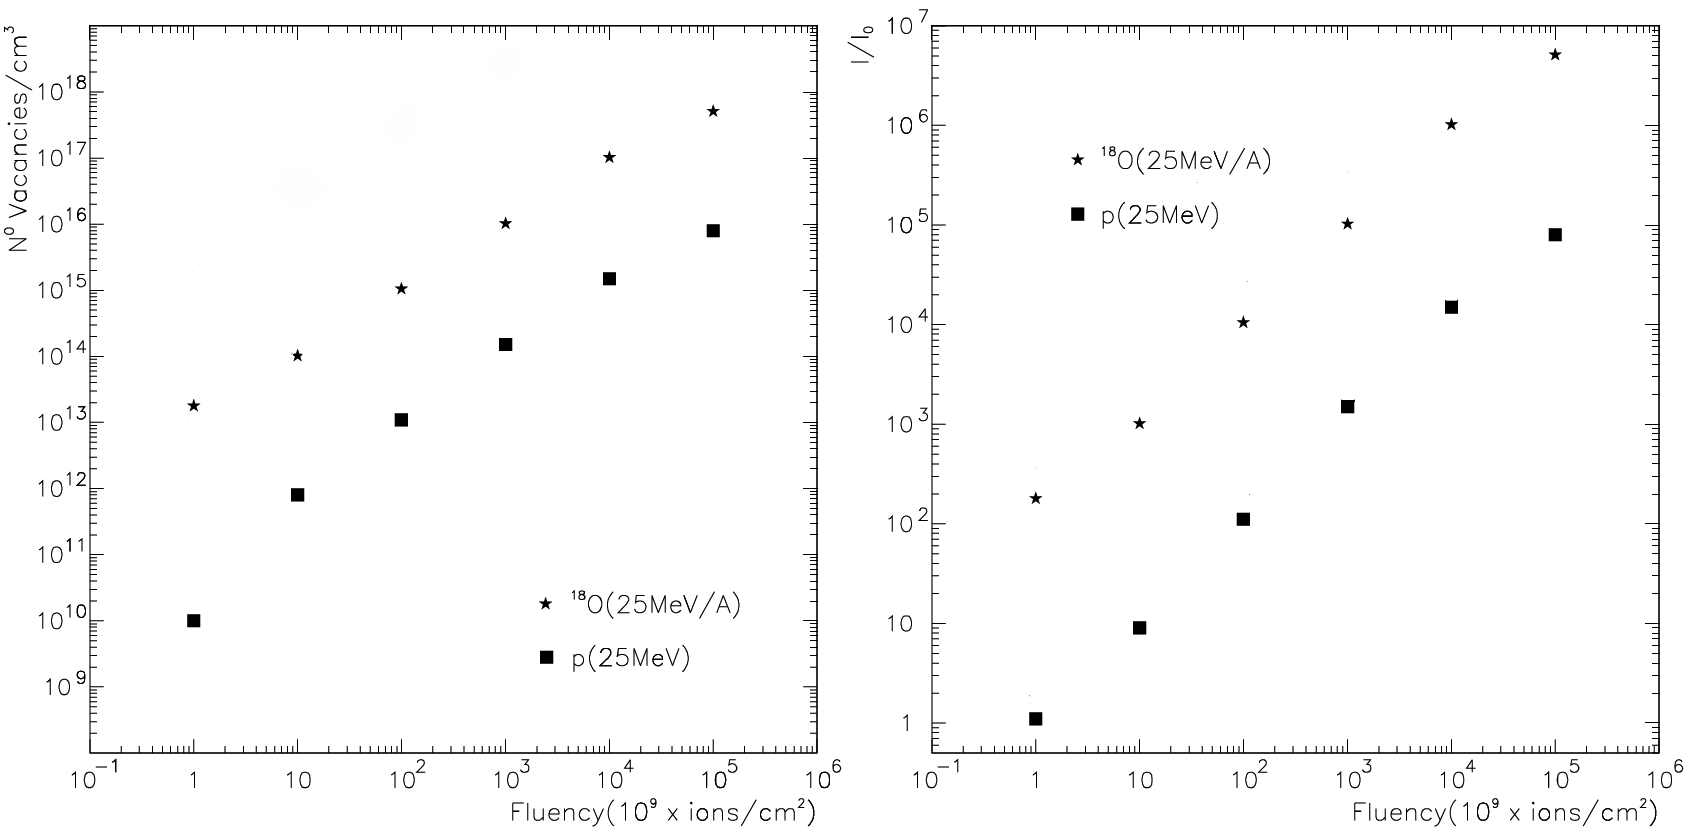
\includegraphics[width=\textwidth, keepaspectratio]{Grafici/sic_simul_resist_radiaz.png}
%	\caption{ Simulazioni Monte Carlo del numero di dislocamenti (a sinistra) e della corrente inversa (a destra) generati in un rivelatore al SiC da 100~$\mu$m in funzione della fluenza di protoni e \ce{^{18}O}. Figura tratta da~\cite{cappuzzello:epja18}.} \label{fig:sic_simul_resist_radiaz}
%\end{figure}



%Gli attuali limiti tecnologici alla produzione di rivelatori al SiC sono legati alla capacità di controllare le dimensioni dell'area attiva e lo spessore dei dispositivi, dal momento che essi vengono realizzati tramite crescita epitassiale su un substrato di SiC.
Gli attuali limiti tecnologici alla produzione di rivelatori al SiC sono legati alla capacità di fabbricare dispositivi con area attiva e spessori relativamente grandi, dal momento che essi vengono realizzati tramite crescita epitassiale su un substrato di SiC.
%Ciò comporta anche la presenza di una regione in cui la ... ZONA PARZIALMENTE VIVA .... NON SO BENE COME INTRODURLA 
Inoltre, la presenza di tale substrato potrebbe rappresentare un problema ai fini della rivelazione, in quanto costituisce uno strato morto in cui le particelle perdono energia senza che questa possa essere misurata o possono perfino fermarsi.
Grazie all'utilizzo di tecniche di ablazione LASER, il substrato potrebbe essere assottigliato fino a pochi~$\mu$m di spessore, ma tale operazione comporta un aumento dei costi, nonché una diminuzione dell'efficienza di produzione, in quanto alcuni dispositivi potrebbero venire danneggiati.
%Inoltre, poiché non è detto che la riduzione del substrato porti significativi benefici, 
Bisogna, dunque, ponderare l'effettiva utilità della riduzione del substrato.
%Tali problematiche sono state tenute in considerazione nella simulazione svolta per questo lavoro di tesi, la quale ne ha valutato l'impatto sulle performance del previsto sistema di rivelazione. 

La simulazione svolta per questo lavoro di tesi ha tenuto in considerazione tali limiti e problematiche, valutandone l'impatto sulle performance del sistema di rivelazione e suggerendo le specifiche tecniche ottimali ai fini del progetto. 






%I due prototipi di rivelatori al SiC utilizzati nel test sono mostrati in Figura~\ref{fig:sic}; essi avevano caratteristiche differenti: uno, chiamato \emph{SiC~A}, aveva un'area attiva non segmentata di $10 \times 10$~mm\ap{2}, con uno spessore di 10~$\mu$m ed uno strato morto di 100~$\mu$m; l'altro, indicato con \emph{SiC~B}, aveva un'area attiva segmentata in quattro pad, ciascuna di $5 \times 5$~mm\ap{2}, con uno spessore di 100~$\mu$m ed un strato morto di 350~$\mu$m.





%I due prototipi di rivelatori al SiC utilizzati nel test presentavano caratteristiche differenti: in primo luogo avevano spessore diversi, poiché uno era spesso 10~$\mu$m, mentre l'altro 100~$\mu$m.

%\vspace{0.5 cm}

\subsection{\iflanguage{italian}{Gli scintillatori allo ioduro di cesio}{Caesium iodide scintillation detector}}





%\subsection{\iflanguage{italian}{I telescopi SiC-CsI}{SiC-CsI telescope detectors}}
I rivelatori a scintillazione, detti anche \emph{scintillatori}, sono tra i più diffusi strumenti per la rivelazione delle particelle.
%Il loro principio di funzionamento è basato sul fatto che quando una particella carica attraversa uno scintillatore vengono emessi fotoni. 
%Il loro principio di funzionamento è basato sull'emissione di luce di scintillazione da parte di certi materiali quando attraversati da una particella carica
Il loro principio di funzionamento è il seguente: quando una particella carica attraversa uno scintillatore, eccita gli atomi o le molecole del materiale, i quali si diseccitano emettendo fotoni. 
La luce prodotta, proporzionale all'energia depositata nel mezzo, viene raccolta e trasformata in segnale elettrico da appositi sensori, come i fotomoltiplicatori o i fotodiodi.
Dal momento che l'energia media necessaria per la creazione di un fotone è circa trenta volte superiore a quella richiesta per la produzione di una coppia elettrone-lacuna in un semiconduttore, la risoluzione energetica tipica degli scintillatori è peggiore di quella dei rivelatori a semiconduttore.
%, con valori tipicamente compresi tra $1 \div 3 \%$.
%I due rivelatori al SiC sono stati assemblati insieme ai due scintillatori allo CsI mostrati in Figura~\ref{fig:csi}. 
%Fra le tipologie più diffuse di scintillatori, lo ioduro di cesio occupa uno dei posti più importanti.

Molti materiali possono produrre luce di scintillazione, differenziandosi per resa in luce, linearità e tempi di decadimento, laddove la resa in luce esprime il numero di fotoni prodotti per unità di energia depositata, la linearità descrive il rapporto di proporzionalità fra la resa in luce e l'energia depositata, il tempo di decadimento indica il tempo necessario per l'emissione di luce dopo il deposito di energia.
Uno dei materiali più diffusi per la realizzazione di rivelatori a scintillazione è lo CsI attivato al Tl, indicato solitamente come CsI(Tl). 
%Dal momento che possiede una fra le maggiori rese in luce e una notevole malleabilità, viene spesso impiegato nella rivelazione sia di particelle cariche sia di raggi gamma.
Dal momento che possiede una fra le maggiori rese in luce e una notevole malleabilità, negli ultimi cinquant'anni ha trovato un largo utilizzo negli esperimenti sia di fisica nucleare sia di fisica particellare, venendo impiegato nella rivelazione di particelle cariche o di raggi gamma.


%La resistenza alle radiazioni dei cristalli di CsI è stata largamente studiata
%Innumerevoli test sono stati condotti per valutare la resistenza alle radiazioni dei cristalli di CsI(Tl), 
%Uno degli aspetti che hanno contribuito alla diffusione dello CsI(Tl) (nel seguito indicato come CsI) è la sua resistenza alle radiazioni, che è stata oggetto di innumerevoli test~\cite{beylin:nima04}. I risultati sono concordi nell'affermare che, sebbene ci siano fluttuazioni legate alla purezza e alle dimensioni dei cristalli, la resa in luce non dovrebbe subire variazioni significative alle intensità di fascio che verranno utilizzate per NUMEN.
%
%Innumerevoli studi sono stati condotti per valutare la resistenza alle radiazioni dello CsI(Tl) (nel seguito indicato come CsI) utilizzando  
%La resistenza alle radiazioni dello CsI(Tl) (nel seguito indicato come CsI) è stata oggetto di innumerevoli test in cui i cristalli venivano irraggiati con raggi gamma o con elettroni.
Uno degli aspetti che ha contribuito alla diffusione dello CsI(Tl) (nel seguito indicato come CsI) è la sua resistenza alle radiazioni, che è stata oggetto di innumerevoli studi in cui i cristalli venivano irraggiati con raggi gamma o con elettroni~\cite{beylin:nima04, zhu:nima98}.
%I risultati sperimentali danno incoraggianti prospettive di sopravvivenza per i cristalli alle intensità di fascio che verranno utilizzate per NUMEN.
%I risultati sono concordi nell'affermare che, sebbene ci siano fluttuazioni legate alla purezza e alle dimensioni dei cristalli, la resa in luce non dovrebbe subire variazioni significative alle intensità di fascio che verranno utilizzate per NUMEN.
Tuttavia, dal momento che in letteratura non sono stati trovati dati sperimentali riguardo la sua resistenza agli ioni pesanti, la collaborazione NUMEN ha svolto specifici test sottoponendo un cristallo di CsI di $ 1 \times 1$~cm\ap{2} ad un fascio di \ce{^{14}N} a 65~AMeV, per una fluenza totale di circa $10^{12}$~particelle/cm\ap{2}, equivalente a circa due anni di esperimento.
Alla fine dell'irraggiamento, il cristallo non presentava danni visibili e la sua resa in luce non mostrava significative variazioni, come si può evincere dalla Figura~\ref{fig:spettro_csi}.
Supportati da questi incoraggianti risultati, la scelta di utilizzare lo CsI sembra promettere le capacità di resistenza alle radiazioni necessarie per NUMEN.

\begin{figure} [!p]
	\centering
	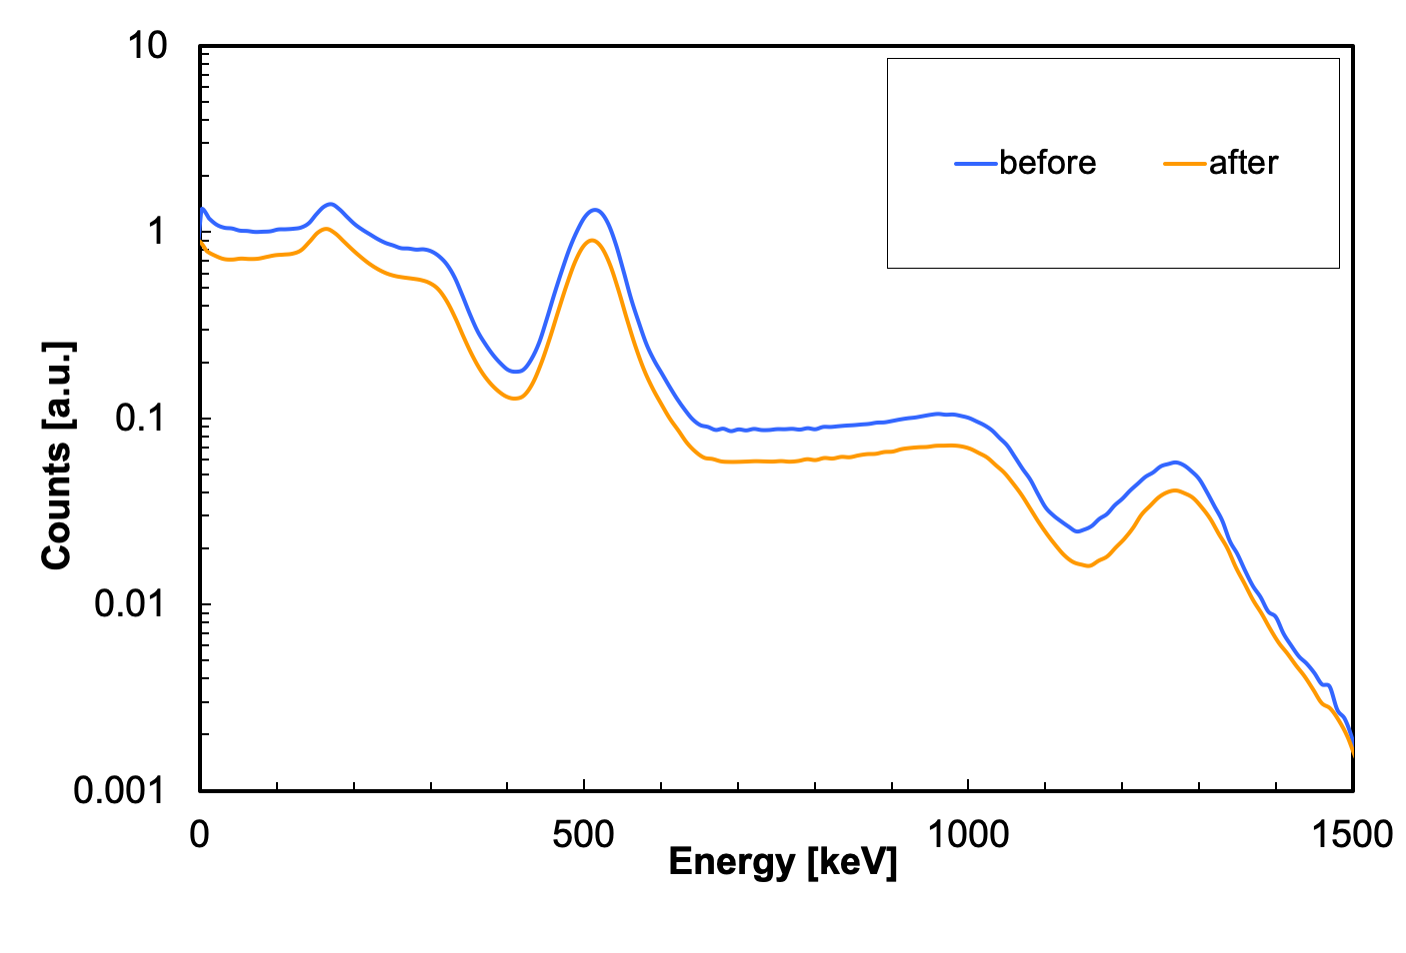
\includegraphics[width=\textwidth, keepaspectratio]{Grafici/spettro_csi.png}
	\caption{Spettro energetico misurato con uno scintillatore allo CsI, prima (blu) e dopo (arancione) un irraggiamento equivalente a circa due anni di esperimento NUMEN.} \label{fig:spettro_csi}
\end{figure}




%\clearpage

%\vspace{0.5 cm}

%\section{\iflanguage{italian}{La configurazione dell'apparato sperimentale nel test}{Experimetal apparatus setting}}
\section{\iflanguage{italian}{Il test beam sui telescopi}{Telescope detectors experimental test}} \label{sez:test}

% ******** QUESTA ERA LA PARTE CHE SECONDO ME VA BENE PER INTRODURRE IL TEST
Ad Aprile 2019 i primi due prototipi di rivelatori al SiC per il progetto NUMEN sono stati completati e resi disponibili dalla ST-Microelectronics. Dal momento che tali dispositivi non sono ancora uno standard nel mondo della fisica ma rappresentano una tecnologia di frontiera, è stato condotto un test per analizzarne la risposta nelle condizioni sperimentali tipiche della Fase~2.
%; una buona risoluzione energetica dello stadio $\Delta E$ di un telescopio è, infatti, essenziale per avere delle buone capacità di PID.

Lo scopo principale del test era valutare la capacità di PID dei telescopi SiC-CsI per gli ioni di interesse, confrontandola con quella dell'attuale sistema basato, sulla combinazione di fili proporzionali e rivelatori al silicio.
%valutandone la capacità di PID nella regione di interesse per NUMEN e confrontandola con quella accessibile con l'attuale apparato. 
%Come illustrato nel Paragrafo~\ref{sez:sistema_identif_part}, i rivelatori al SiC sono stati scelti nell'ambito del progetto come stadio~$\Delta E$ di un telescopio SiC-CsI per l'identificazione in numero atomico dei prodotti di reazione. Lo scopo principale del test era, dunque, valutare la capacità di PID di questo sistema nella regione di interesse per NUMEN, confrontandola con quella accessibile con l'attuale apparato.
In aggiunta, poiché l'upgrade del FPD prevede anche la sostituzione dell'elettronica attualmente utilizzata con una basata su chip VMM3a~\cite{degeronimo:ieee13}, il test aveva anche l'obiettivo di valutare le prestazioni del primo prototipo di elettronica di front-end prevista per NUMEN.
Ciò ha, inoltre, permesso di effettuare un confronto delle performance dei telescopi in funzione dell'elettronica adoperata.

Il test è stato svolto ai LNS utilizzando un fascio di~\ce{^{20}Ne} a 20~AMeV, incidente su \ce{^{197}Au} o \ce{^{12}C}, laddove i due bersagli avevano funzioni differenti: il primo serviva per massimizzare eventi di scattering elastico, il secondo per favorire la formazione dei prodotti di reazione di interesse.
%, ovvero quella dell'O, del F e del Ne.




%\vspace{0.5 cm}


\subsection{\iflanguage{italian}{I telescopi utilizzati nel test}{Telescope detectors used in the test}}

\begin{figure} [!p]
	\centering
	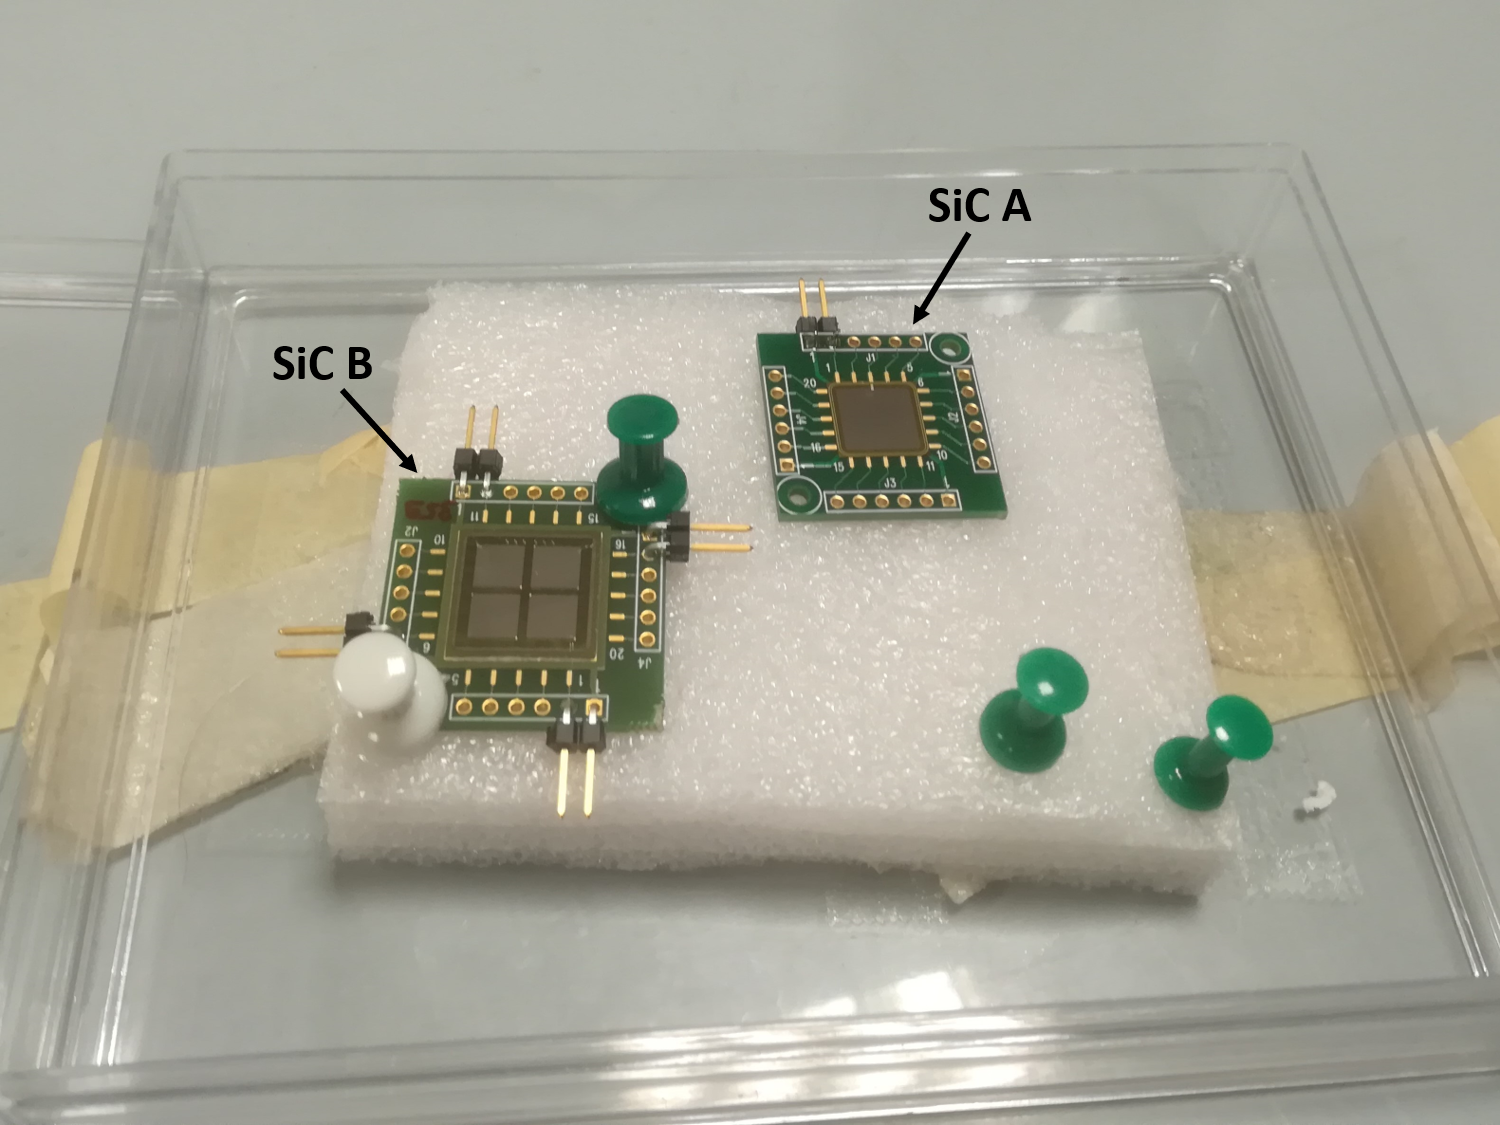
\includegraphics[width=\textwidth, keepaspectratio]{Grafici/sic_etichette.png}
	\caption{I rivelatori al carburo di silicio (SiC) utilizzati nel test: a sinistra il \emph{SiC~B}, a destra il \emph{SiC~A}.} \label{fig:sic}
\end{figure}

I due prototipi di rivelatori al SiC utilizzati nel test sono mostrati in Figura~\ref{fig:sic}: come è possibile notare, essi differiscono innanzitutto per la segmentazione dell'area attiva, in quanto uno (\emph{SiC~A}) è costituito da un'unica pad, mentre l'altro (\emph{SiC~B}) è suddiviso in quattro regioni. 
%Inoltre, mentre il SiC~A aveva un'area attiva di $10 \times 10$~mm\ap{2}, il SiC~B presentava 
%I due telescopi SiC-CsI utilizzati nel test
Entrambi i rivelatori hanno un'area attiva complessiva di $10 \times 10$~mm\ap{2}, laddove ogni pad del SiC~B ha un'estensione di $5 \times 5$~mm\ap{2}.
%Un'ulteriore differenza riguardava gli spessori dei due rivelatori: mentre il SiC~A era spesso 10~$\mu$m con 100~$\mu$m di strato morto, il SiC~B aveva uno spessore di 100~$\mu$m con 350~$\mu$m di .
Un'ulteriore differenza riguarda lo spessore della regione attiva dei due rivelatori: per il SiC~A è di 10~$\mu$m, mentre per il SiC~B misura 100~$\mu$m.
Infine, entrambi i rivelatori hanno un substrato morto, che per il SiC~A è spesso 100~$\mu$m, invece per il SiC~B ha uno spessore di~350~$\mu$m.
In occasione del test si è scelto di utilizzare soltanto due delle quattro pad del SiC~B, le quali sono state cortocircuitate tra loro in modo che questo rivelatore avesse una superficie sensibile di $10 \times 5$~mm\ap{2}.





%\vspace{3 cm}


\begin{figure} [!t]
	\centering
	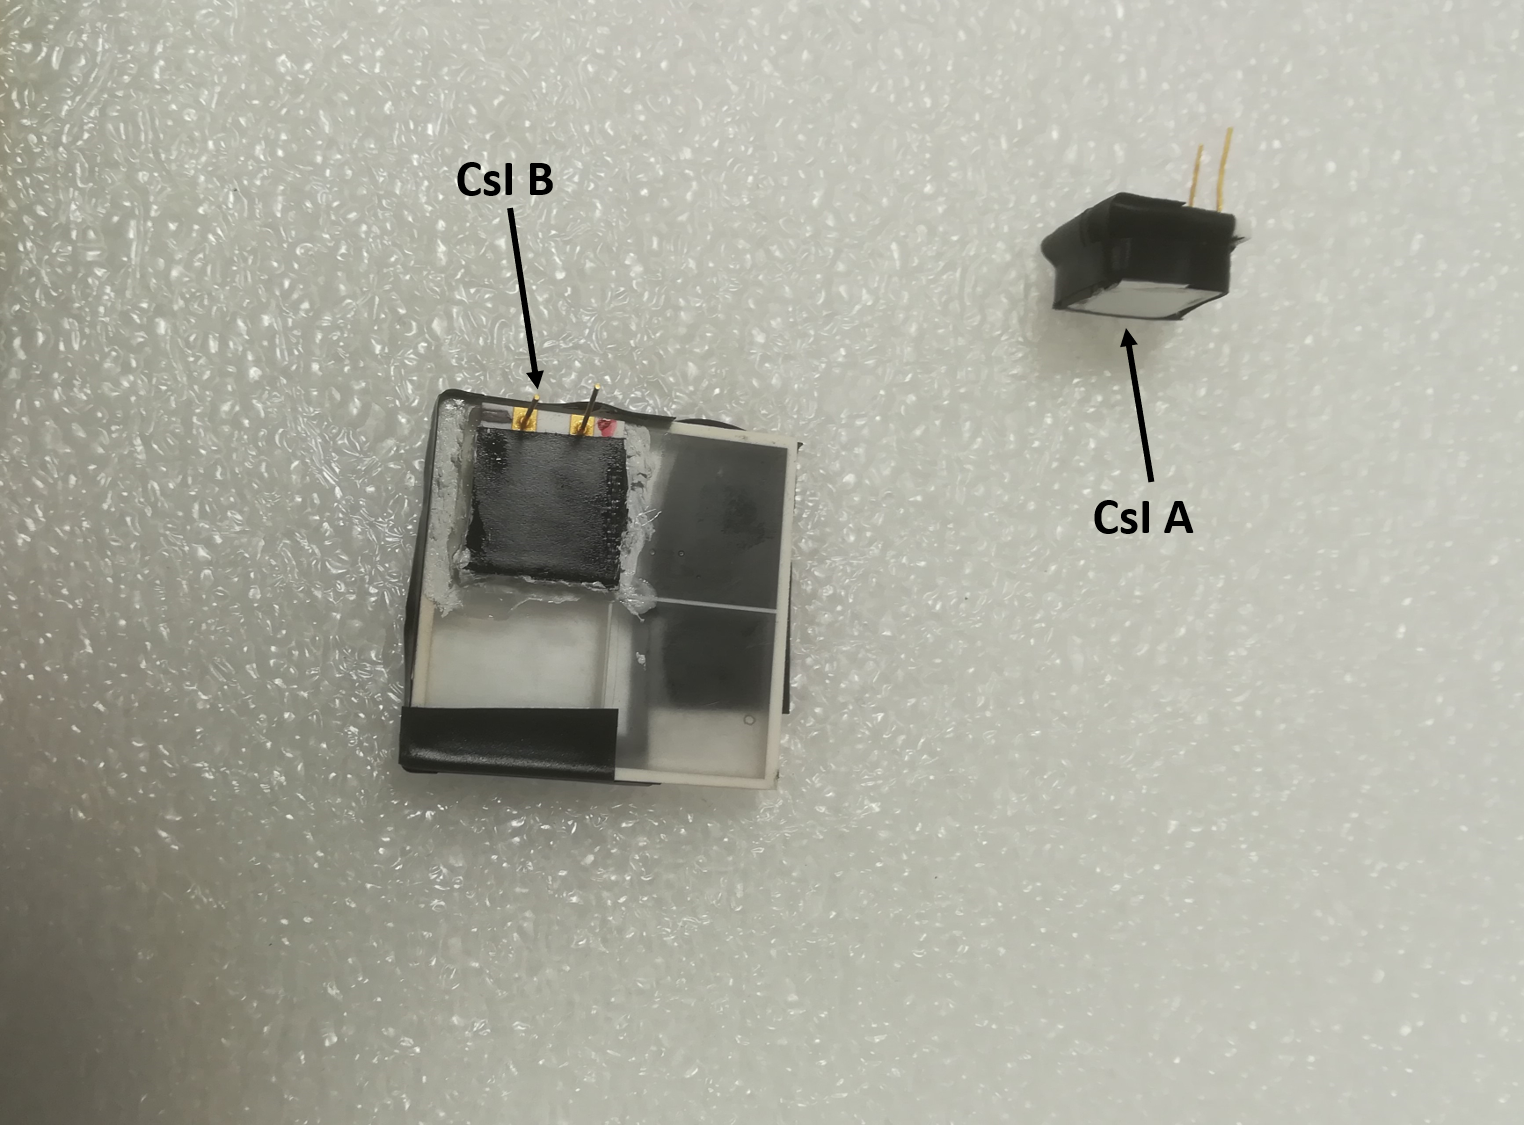
\includegraphics[scale=0.5]{Grafici/csi_etichette.png}
	\caption{I rivelatori a scintillazione utilizzati nel test: a sinistra il \emph{CsI~B}, a destra il \emph{CsI~A}. Guardando, ad esempio, il CsI~B, si possono notare lo scintillatore (CsI), che appare come un materiale trasparente, e il fotodiodo, che si trova coperto dal nastro isolante nero per migliorare la schermatura. Inoltre, è possibile vedere anche il Mylar bianco con cui sono stati rivestiti i cristalli.} \label{fig:csi}
\end{figure}



%In occasione del test sono stati utilizzati due scintillatori allo CsI, i quali sono mostrati in Figura~\ref{fig:csi}.
Gli scintillatori allo CsI utilizzati nel test sono mostrati in Figura~\ref{fig:csi}.
Essi hanno dimensioni differenti: uno (\emph{CsI~A}) è da $1 \times 1$~cm\ap{2}, l'altro (\emph{CsI~B}) è suddiviso in quattro regioni da $1.5 \times 1.5$~cm\ap{2}. 
%La luce di scintillazione veniva letta in entrambi i casi con un fotodiodo da $1 \times 1$~cm\ap{2}, che 
%Ognuno dei due scintillatori era accoppiato ad un fotodiodo $1 \times 1$~cm\ap{2}
A causa delle dimensioni dei rivelatori al SiC, soltanto una delle quattro aree sensibili del CsI~B è stata utilizzata. Per migliorare la raccolta della luce, i cristalli sono stati avvolti con del Mylar bianco, il quale è stato fissato con del nastro isolante nero.
%
%I cristalli sono stati avvolti con del mylar e del nastro isolante nero per migliorare la raccolta della luce.
%
Ciascuno scintillatore era accoppiato tramite grasso ottico ad un fotodiodo di area $1 \times 1$~cm\ap{2} per la lettura della luce di scintillazione. 



\begin{figure} [!t]
	\centering
	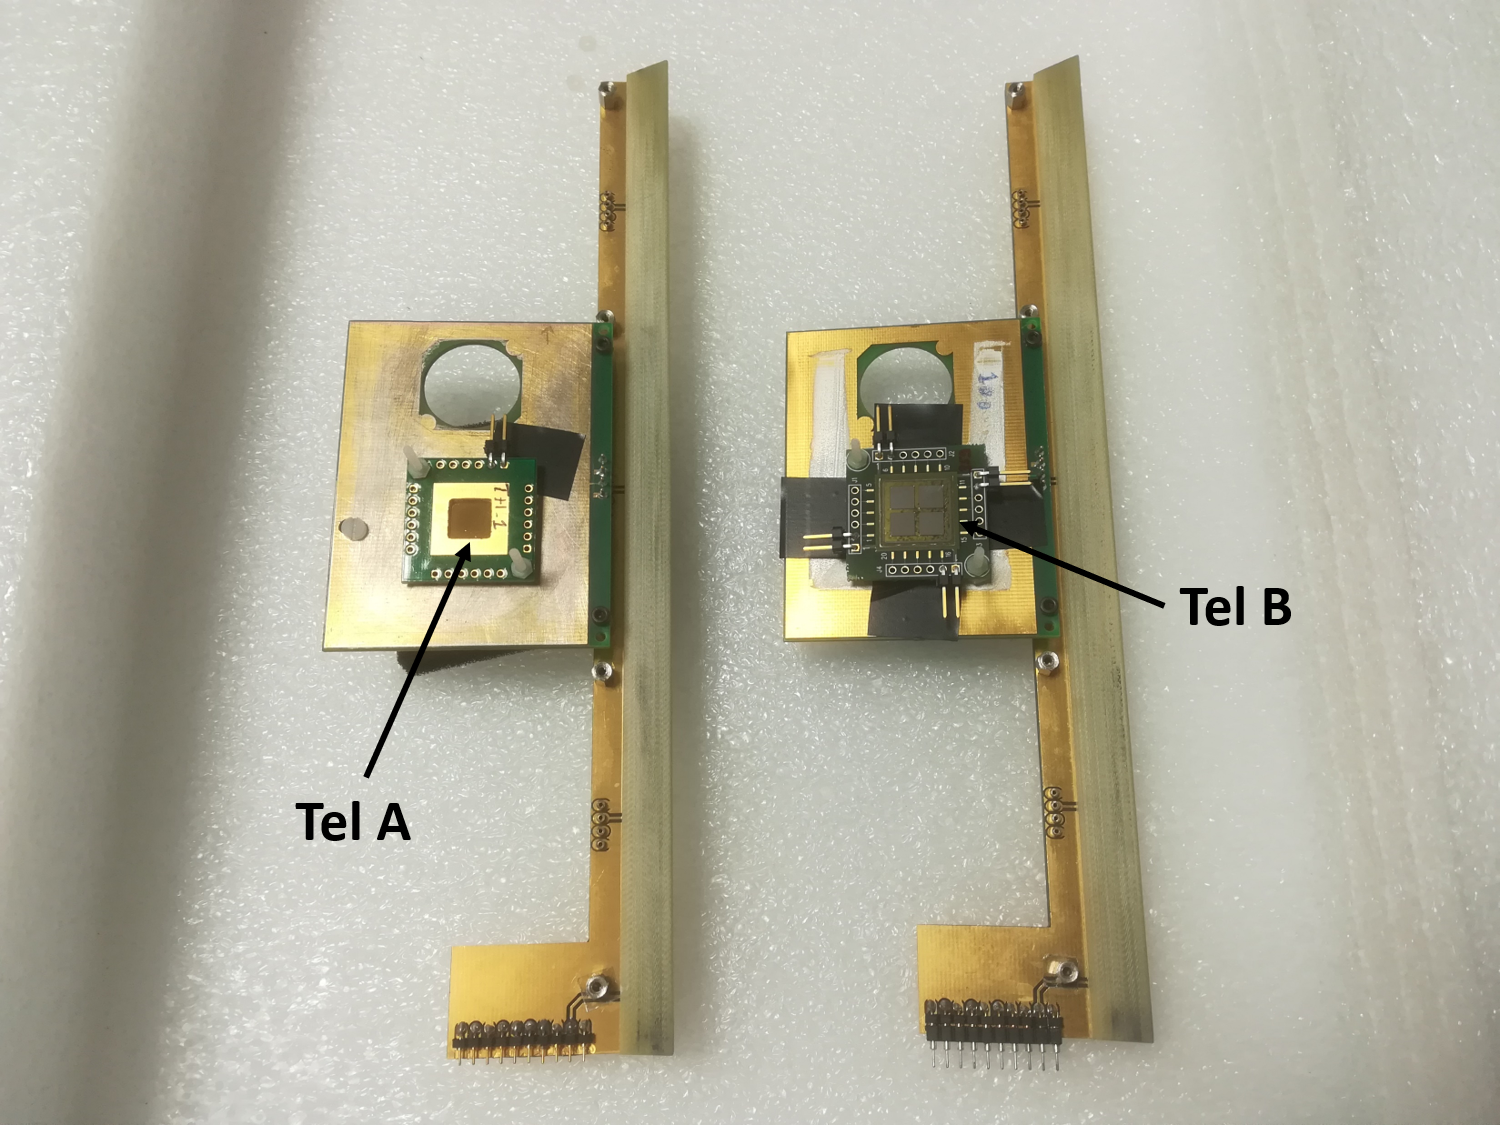
\includegraphics[scale=0.5]{Grafici/telescopi_etichette.png}
	\caption{I due telescopi SiC-CsI utilizzati nel test: a sinistra il \emph{Tel~A}, a destra il \emph{Tel~B}.} \label{fig:telescopi}
\end{figure}






Il SiC~A e il SiC~B sono stati assemblati, rispettivamente, con il CsI~A e il CsI~B, così da formare i due telescopi (\emph{Tel~A} e \emph{Tel~B}) mostrati in Figura~\ref{fig:telescopi}.
%; in particolare, mentre nel Tel~A il SiC~A era \emph{reverse mounted}, nel Tel~B il SiC~B era \emph{direct mounted} (\textcolor{red}{va bene detto così?}).
Al fine di ottenere una migliore correlazione $\Delta E - E_{resid}$, il SiC~A è stato montato in configurazione \emph{reverse}, ovvero rivolgendo alle particelle incidenti prima il substrato morto e poi la regione sensibile.
Ciò non è stato possibile per il SiC~B a causa del maggiore substrato morto che avrebbe fermato gli ioni.
%I due telescopi, fissati su due delle strutture che solitamente ospitano i rivelatori al silicio, sono stati posti nel FPD secondo lo schema riportato in Figura.
%Come si può notare, quattro rivelatori al silicio sono stati montati in modo simmetrico rispetto al SiC~A, in modo da avere un utile riferimento sia per la fase di acquisizione sia per l'analisi offline.
%Come si può notare, a sinistra e a destra del Tel~A sono stati montati due rivelatori al silicio, in modo da avere un utile riferimento sia per la fase di acquisizione sia per l'analisi offline.
Dunque, all'energia utilizzata nel test, gli ioni incidenti sul Tel~B venivano arrestati nel substrato del SiC~B, per cui da questo telescopio era possibile estrarre soltanto l'informazione sul $\Delta E$.

I due telescopi, fissati su schede in PCB, sono stati posti nel FPD di MAGNEX in due delle colonne che solitamente ospitano i rivelatori al silicio.
%A sinistra e a destra del Tel~A sono stati montati due rivelatori al silicio, in modo da avere un utile riferimento sia per la fase di acquisizione sia per l'analisi offline.
Insieme ai due telescopi sono stati montati quattro rivelatori al silicio: due erano posizionati fra il Tel~A e il Tel~B, e due a sinistra del Tel~A.
Questi avevano lo scopo di fornire un riferimento durante l'acquisizione dei dati sperimentali ed essere un metro di paragone per le capacità di PID in fase di analisi.









%\subsection{\iflanguage{italian}{Configurazione dell'apparato sperimentale}{Setting of the experimental apparatus}}
\subsection{\iflanguage{italian}{Le catene elettroniche del test}{The electronic chains used in the test}}


%La catena elettronica 
%Dal momento che il test aveva anche lo scopo di valutare le differenze di risposta dei telescopi SiC-CsI a seconda dell'elettronica utilizzata, sono state montate due diverse catene elettroniche:
Dal momento che il test aveva anche lo scopo di valutare le differenze di risposta dei telescopi SiC-CsI a seconda dell'elettronica utilizzata, il Tel~A è stato equipaggiato con due diverse catene elettroniche:
la prima (\emph{standard}) rispecchia quella attualmente adoperata per i rivelatori al silicio, la seconda (\emph{VMM3a}) era incentrata sul prototipo di chip VMM3a.
%, a cui ci si riferisce come \emph{elettronica~Boiano} nel caso dell'elettronica attualmente adoperata e come \emph{elettronica~VMM3} nel caso di quella prevista per NUMEN.
%La catena elettronica del sistema fili+silici non è discussa nel presente lavoro di tesi
%Dunque, nel presente lavoro di tesi viene
I fili proporzionali e i rivelatori al silicio utilizzati nel test hanno, invece, montato l'elettronica tradizionale, la quale, essendo stata ampiamente discussa in numerose pubblicazioni, non verrà illustrata nel presente lavoro di tesi.
%Poiché l'elettronica standard di MAGNEX è stata ampiamente discussa in numerose pubblicazioni, nel presente lavoro di tesi vengono illustrate soltanto le catene elettroniche relative al Tel~A.
%Il tracciatore a gas e i rivelatori al silicio utilizzati nel test hanno montato la catena elettronica standard, di cui nel presente lavoro di tesi 
Dunque, nel seguito verranno descritte soltanto le due catene elettroniche relative al Tel~A.
%In entrambe le configurazioni, il trigger per l'acquisizione del segnale del telescopio era fornito dal CsI~A, il quale era inviato 

%È bene precisare che, mentre per i rivelatori al silicio sono stati usati PA da 5~mV/MeV, per il rivelatore al SiC e per lo scintillatore allo CsI sono stati utilizzati PA da 45~mV/MeV. 


%Nella catena elettronica standard, di cui in Figura si riporta uno schema, il segnale proveniente dal rivelatore era inviato ad un preamplificatore (PA) di carica~\cite{boiano:ieee08}.
%Sia per il rivelatore al SiC sia per lo scintillatore allo CsI sono stati utilizzati PA con sensibilità di 45~mV/MeV.
%Nella catena elettronica standard, di cui in Figura si riporta uno schema, i segnali provenienti dai due stadi del telescopio erano rispettivamente inviati a due preamplificatori (PA) di carica~\cite{boiano:ieee08} con sensibilità di 45~mV/MeV.

\paragraph{Elettronica standard} 
Nella catena elettronica standard, di cui in Figura~\ref{fig:elettronica_standard} si riporta uno schema, il segnale proveniente dal SiC~A era inviato ad un preamplificatore (PA) di carica~\cite{boiano:ieee08} con sensibilità di 45~mV/MeV.
Questo, oltre a raccogliere ed integrare il segnale, era utilizzato anche per fornire la tensione di alimentazione al rivelatore, pari a $-50$~V, generata da un alimentatore esterno.
%L'output del PA era collegata ad un amplificatore MEGAMP.
%L'uscita del MEGAMP era inviata all'ADC per l'acquisizione.
%L'output del PA era collegato ad un amplificatore MEGAMP a 16 canali, che, oltre ad amplificare il segnale, ne modificava la forma in modo da renderlo gaussiano.
%L'output del PA era collegato ad un amplificatore formatore MEGAMP a 16 canali, il quale possedeva due tipologie di uscite: una restituiva un segnale analogico,  impiegato per la misura dell'energia, l'altra produceva un segnale logico da discriminatore a frazione costante (Constant Fraction Discriminator, CFD), solitamente utilizzato per misure di tempo o per la creazione del gate.
L'output del PA era collegato ad un amplificatore formatore MEGAMP a 16 canali, il quale in un unico modulo riunisce amplificatore e discriminatore a frazione costante (Constant Fraction Discriminator, CFD); esso, infatti, possiede per ogni ingresso due tipologie di uscita: una restituisce un segnale analogico, tipicamente impiegato per la misura dell'energia, l'altra produce un segnale logico, solitamente utilizzato per misure di tempo o per la creazione del gate.
%
%
%Mentre la prima è tipicamente impiegata per la spettroscopia, 
%L'uscita del PA era, infine, inviata all'ADC per l'acquisizione dell'informazione sulla perdita di energia~$\Delta E$.
%Dal MEGAMP veniva, in questo caso, prelevato soltanto il segnale analogico, il quale, formato con uno shaping time di 500~ns.
In questo ramo della catena, dal MEGAMP veniva prelevato soltanto il segnale analogico, per il quale si era scelto uno shaping time di 500~ns.
Tale segnale era, infine, inviato all'ADC di picco per l'acquisizione dell'informazione sulla perdita di energia~$\Delta E$.
%
%Il segnale prodotto dal fotodiodo era collegato ad un PA analogo a quello utilizzato per il rivelatore al SiC.
%Dal momento che il segnale dello scintillatore era utilizzato per dare il trigger,

Per quanto riguarda il CsI~A, il segnale di output del fotodiodo era raccolto da un PA analogo a quello utilizzato per il SiC~A.
La tensione di alimentazione del fotodiodo, pari a $-70$~V, era fornita, anche in questo caso, tramite il PA e generata da un alimentatore esterno.
L'uscita del PA era inviata al MEGAMP, da cui venivano estratti due segnali: quello analogico era inviato direttamente all'ADC di picco per l'acquisizione dell'energia residua $E_{resid}$, quello del CFD veniva sdoppiata in due copie, di cui una era utilizzata per dare il gate all'acquisizione dei segnali del telescopio, mentre l'altra era inviata al modulo OR che produce il Master Trigger per l'acquisizione. 
A tale modulo erano collegati anche i segnali logici provenienti dalle catene elettroniche dei quattro rivelatori al silicio, in modo da consentire un'acquisizione parallela dei segnali standard di MAGNEX e di quelli del telescopio.

%utilizzato per dare il trigger all'acquisizione dei segnali del telescopio.

\begin{figure} [!p]
	\centering
	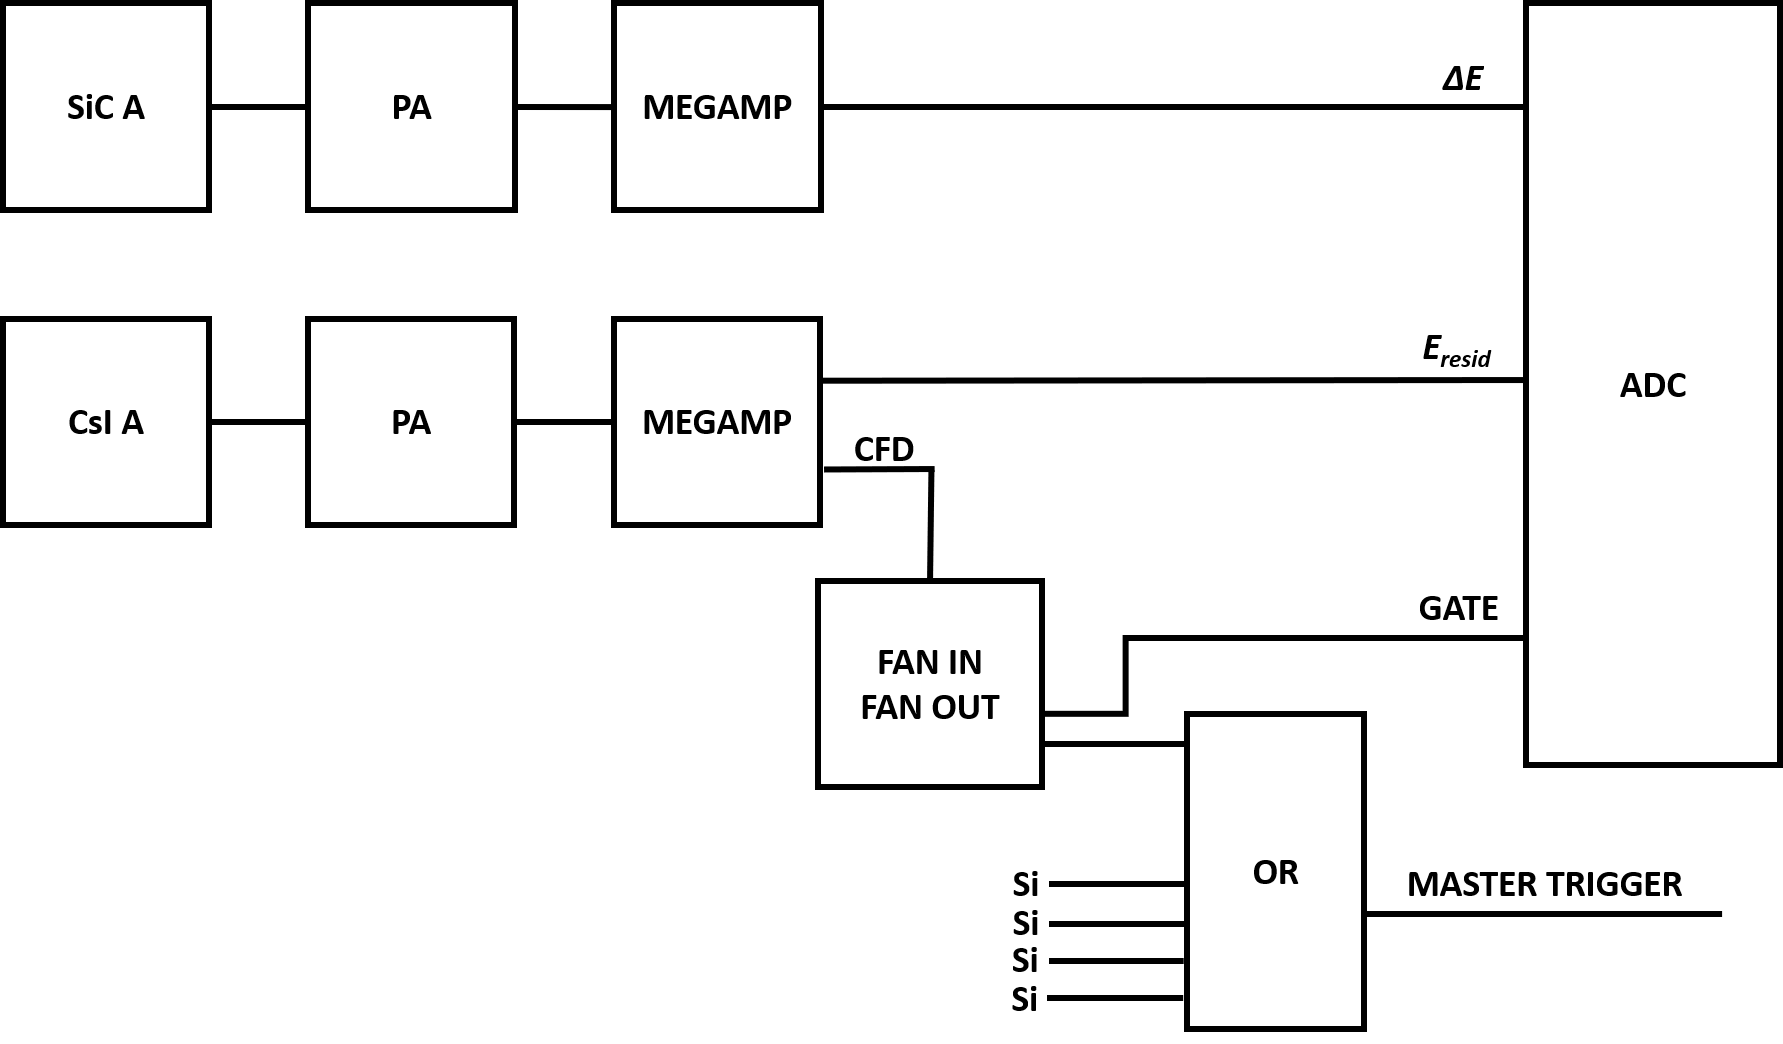
\includegraphics[width=\textwidth, keepaspectratio]{Grafici/elettronica_standard.png}
	\caption{L'elettronica \emph{standard} associata al Tel~A.} \label{fig:elettronica_standard}
\end{figure}

%\clearpage


\paragraph{Elettronica VMM3a} 
%Nella catena elettronica VMM3, il cui schema è illustrato in Figura~\ref{fig:elettronica_vmm}, il segnale del SiC~A era inviato direttamente al chip VMM3, il quale racchiudeva in sé un PA da $3 \div 6$~mV/fC e un amplificatore formatore con shaping time da 200~ns.
%
Nella catena elettronica VMM3a, il cui schema è illustrato in Figura~\ref{fig:elettronica_vmm}, il segnale del SiC~A era inviato direttamente al chip VMM3a, che, sviluppato in origine per l'esperimento ATLAS, è stato adattato per gli scopi di NUMEN.
Possedendo un'architettura a 64~canali, esso consente una più semplice gestione di apparati con un grande numero di canali.
%
%
%Tale chip possiede 64 canali e, per ogni canale, è capace di fornire informazioni sull'ampiezza del picco e sul timing del segnale. 
%La sensibilità del PA poteva essere selezionata nel range $3 \div 6$~mV/fC. 
%Tale chip possedeva un'architettura a 64~canali, consentendo, dunque, una più semplice gestione di apparati con un grande numero di canali.
Dal momento che il futuro muro per la PID prevede l'utilizzo di 1230 telescopi, la scelta di un'elettronica di front-end con questo tipo di caratteristiche è essenziale in termini di facilità di controllo dei dispositivi, di economia degli spazi e di più semplice dissipazione del calore.
%Per ogni canale, il chip poteva restituire l'informazione sul canale di provenienza, sull'ampiezza del picco e sul timing del segnale.
Per ogni canale il chip racchiude in sè un PA da $3 \div 6$~mV/fC e un amplificatore formatore con shaping time da $25 \div 200$~ns.
La scheda è, inoltre, dotata di un'uscita monitor, attraverso la quale è possibile osservare il segnale analogico formato dal circuito amplificatore.

Il VMM3a era collegato alla scheda di read-out System On Module (SOM) della National Instruments~\cite{national_instruments}.
%, che univa un efficace Field Programmable Gate Array (FPGA) ad un potente processore.
%Il compito principale della SOM era la lettura veloce dei segnali provenienti dal VMM3
Nella prospettiva della Fase~4, la SOM deve assicurare la lettura veloce dei segnali provenienti dal VMM3a e il trasferimento rapido dei dati al sistema di acquisizione tramite una connessione Gb~Ethernet.
Tali obiettivi saranno possibili grazie alla struttura della SOM, che unisce un efficace Field Programmable Gate Array (FPGA) ad un potente processore.
In Figura~\ref{fig:vmm+som} è riportata una foto del chip VMM3a e della scheda SOM utilizzati nel test.

Dal momento che all'oscilloscopio si era notato che il segnale di output della SOM era in anticipo rispetto al gate (dato dal CsI~A), il primo era inviato ad una linea di ritardo passiva da 140~ns. Infine, il segnale giungeva all'ADC per l'acquisizione.

%Il segnale di output della SOM, opportunamente ritardato di 140~ns, era inviato all'ADC, dove veniva acquisito.

Per quanto concerne il CsI~A, il segnale del fotodiodo era inviato al VMM3a, da cui, in questo caso, venivano estratti due segnali: uno, analogico, era dato in input alla SOM, l'altro, logico, veniva utilizzato per la formazione del gate. 
Poiché l'ADC utilizzata richiedeva in ingresso un gate negativo mentre il segnale logico prodotto dalla SOM era positivo, quest'ultimo era prima inviato ad un modulo Fan~in/Fan~out, da cui si prelevava l'uscita invertente (INV).
Dal momento che l'inversione del segnale richiedeva del tempo di elaborazione, il segnale analogico risultava in anticipo rispetto al gate. Anche in questo caso è stato, dunque, necessario ritardare opportunamente il segnale di output della SOM prima di inviarlo all'ADC.
Un'altra copia del segnale del CFD era inviata al modulo OR utilizzato per la generazione del Master Trigger, nel quale, come nella configurazione precedentemente discussa, giungevano anche i segnali logici delle catene dei rivelatori al silicio.
Pertanto, anche in questo set-up venivano registrati i segnali standard di MAGNEX.

\begin{figure} [!p]
	\centering
	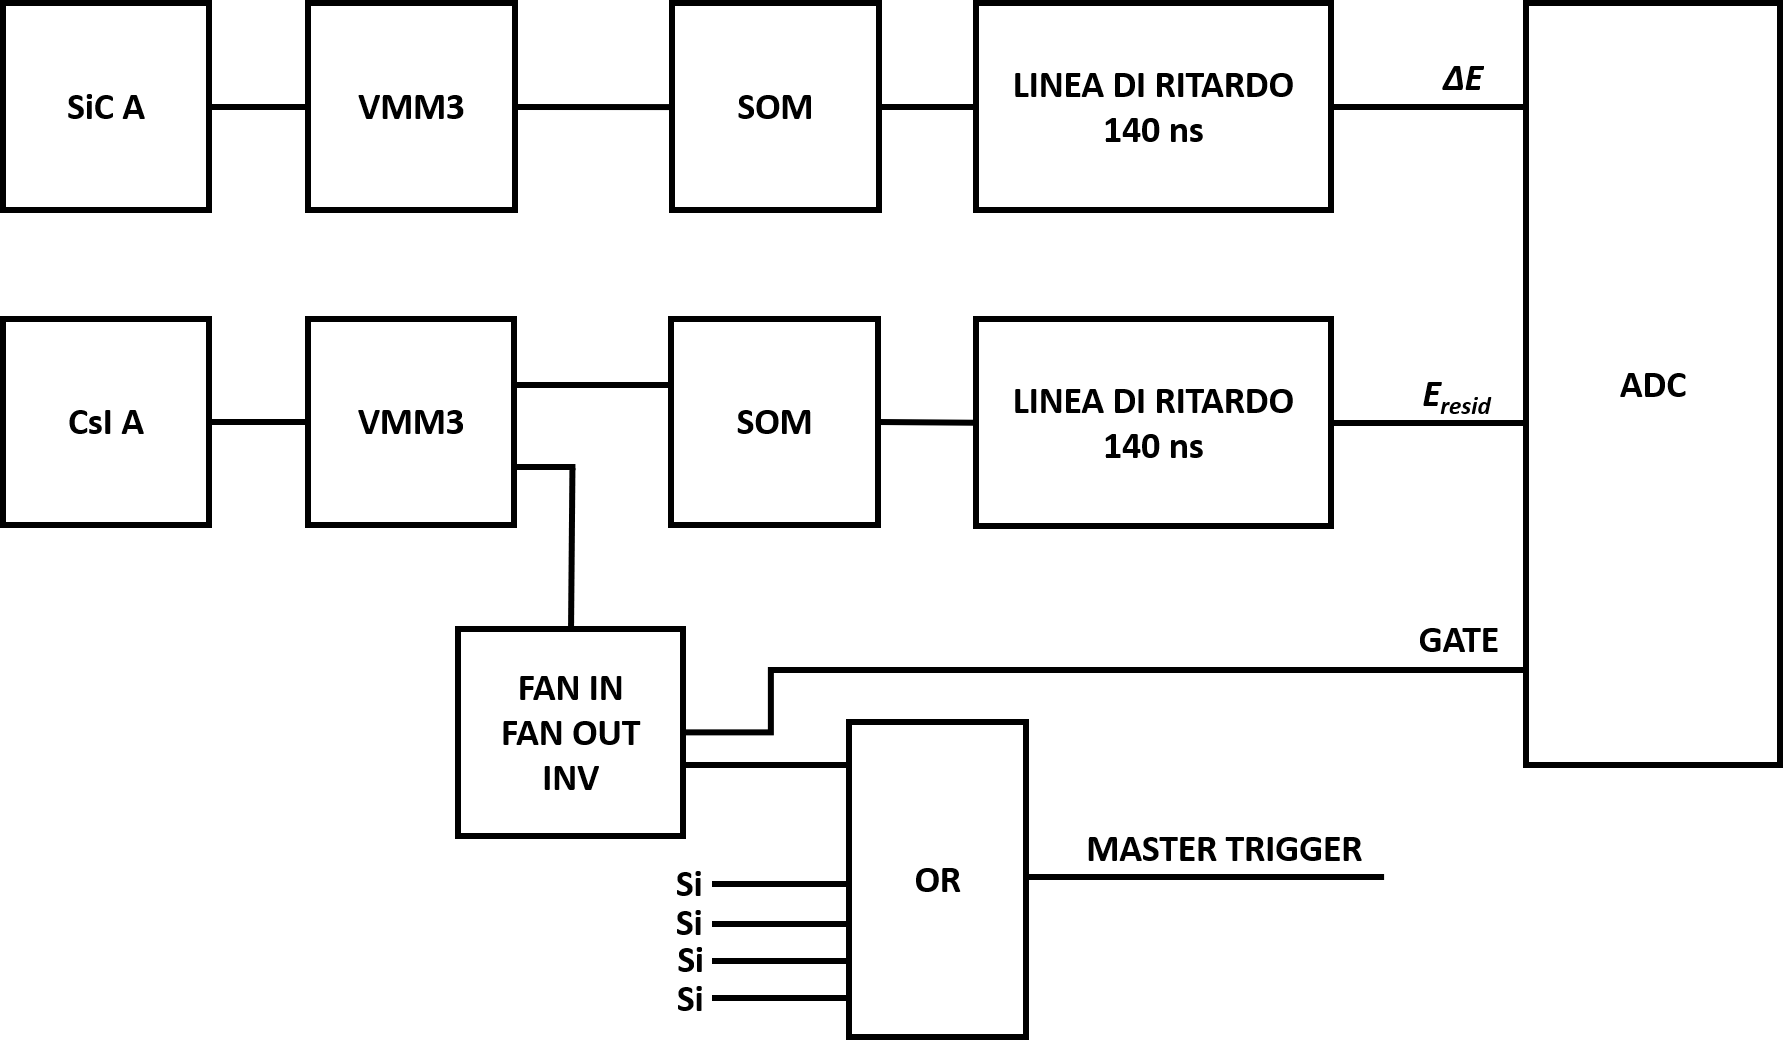
\includegraphics[width=\textwidth, keepaspectratio]{Grafici/elettronica_vmm.png}
	\caption{L'elettronica \emph{VMM3a} associata al Tel~A.} \label{fig:elettronica_vmm}
\end{figure}

\begin{figure} [!p]
	\centering
	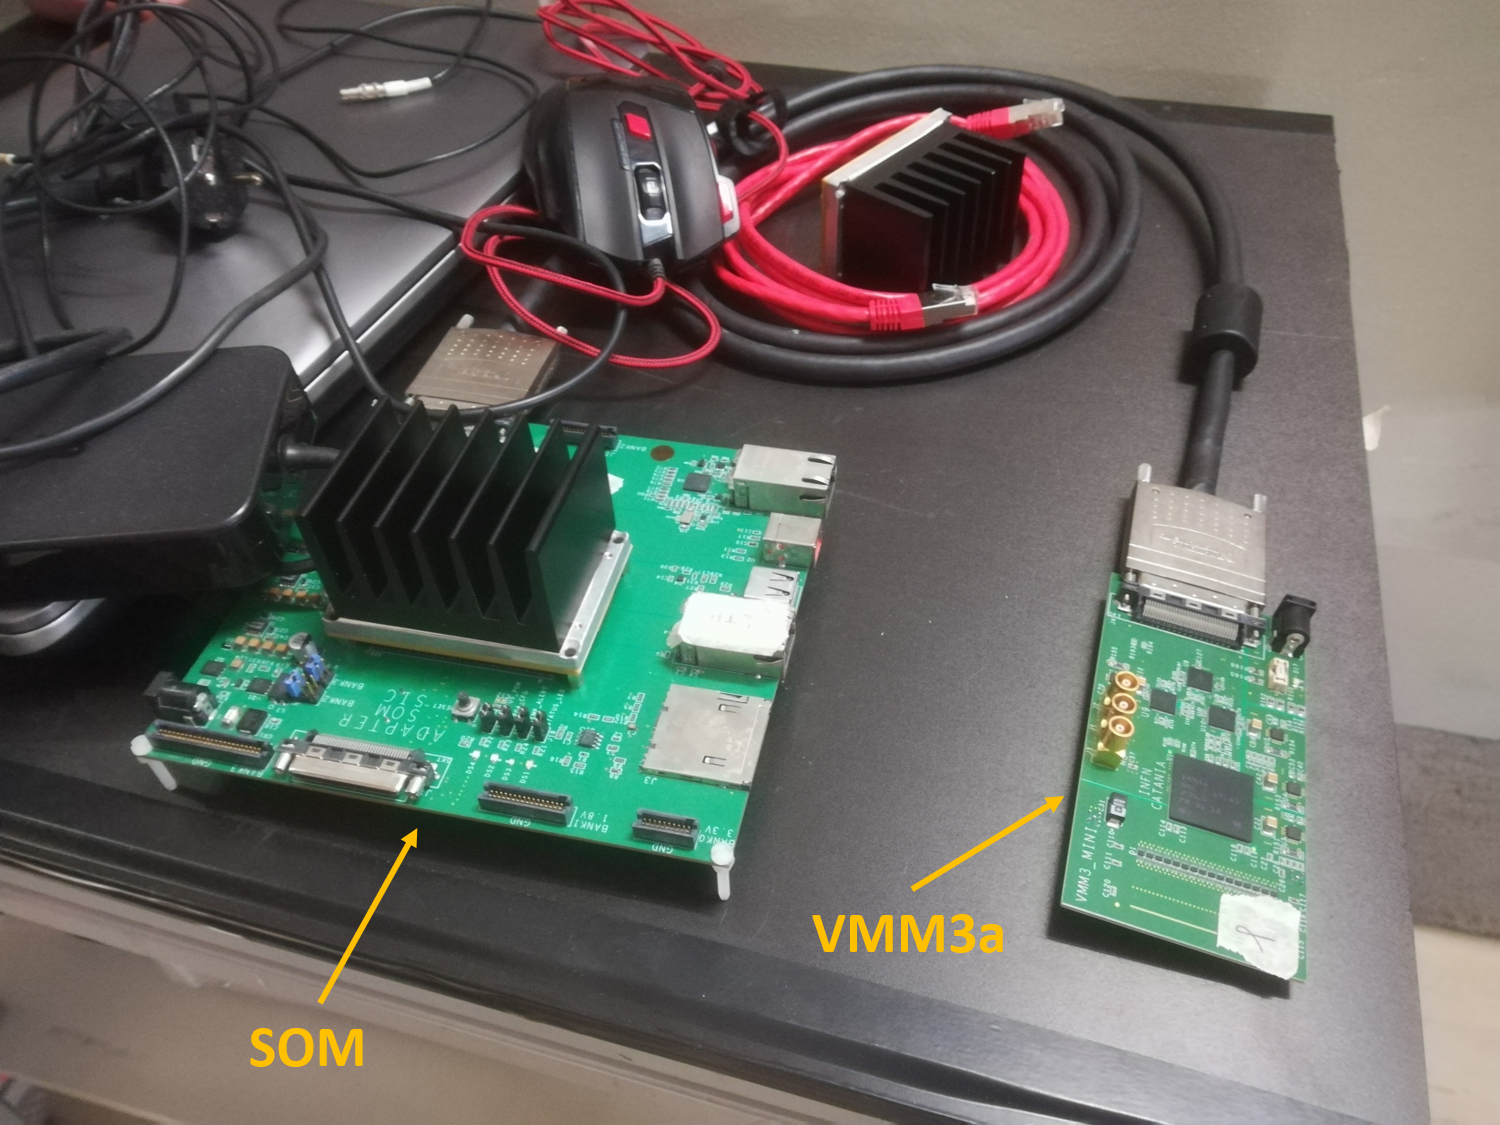
\includegraphics[width=\textwidth, keepaspectratio]{Grafici/vmm3a_som.png}
	\caption{Il chip VMM3a e la scheda SOM utilizzati nel test.} \label{fig:vmm+som}
\end{figure} 


\chapter{\iflanguage{italian}{La simulazione}{The simulation}} \label{cap:simulazione}




%Al fine di valutare se la scelta della tecnologia SiC-CsI può soddisfare le esigenze di NUMEN è stata implementata una simulazione Monte Carlo sulla piattaforma GEANT4.
%In questo capitolo vengono esposte le principali assunzioni e vengono presentati i risultati.



%Nei moderni esperimenti di fisica l'importanza delle simulazioni computerizzate è andata via via crescendo grazie all'eccezionale sviluppo dei computer e dei software volti a tale scopo; in particolare, l'introduzione delle tecniche Monte Carlo si è rivelata un potente strumento per trattare problemi complessi altrimenti difficilmente risolubili.
Nei moderni esperimenti di fisica l'importanza delle simulazioni numeriche è cresciuta senza sosta grazie all'eccezionale sviluppo dei computer e dei software di simulazione; in particolare, l'introduzione delle tecniche Monte Carlo si è rivelata un potente strumento per trattare problemi complessi altrimenti difficilmente risolubili.
In questo capitolo, dopo aver descritto le principali caratteristiche di tali metodi, si discute brevemente della piattaforma \geant, con la quale sono state implementate le simulazioni svolte per questo lavoro di tesi.

%Successivamente, vengono presentati gli aspetti più importanti di tali simulazioni, le quali avevano lo scopo di valutare se la scelta di utilizzare dei telescopi basati sulla tecnologia SiC-CsI può soddisfare le esigenze di NUMEN.
%Successivamente, dopo aver presentato gli aspetti più importanti di tali simulazioni, vengono discussi i risultati ottenuti, illustrando nei diversi casi le matrici $\Delta E - E$ e calcolando la percentuale di errore nell'identificazione degli ioni simulati.
Successivamente, dopo aver spiegato gli aspetti più importanti di tali simulazioni, vengono discussi i risultati ottenuti, evidenziando nei diversi casi le conseguenze sulle performance di Particle IDentification (PID).



%Le simulazioni giocano un ruolo fondamentale nella fisica.

%In fisica, come in altre scienze, le simulazioni giocano un ruolo fondamentale, in quanto permettono di studiare la risposta di sistemi complessi tenendo sotto controllo alcuni dei suoi gradi di libertà.

\section{\iflanguage{italian}{Le simulazioni computerizzate e i metodi Monte Carlo}{Computer simulations and Monte-Carlo methods}}


In fisica, come in altre scienze, le simulazioni computerizzate giocano un ruolo fondamentale, in quanto permettono di affrontare lo studio di sistemi che sarebbero difficilmente trattabili utilizzando tecniche teoriche o sperimentali~``classiche'';
spesso, infatti, questi approcci possono presentare problematicità legate alla complessità del sistema, al tempo necessario per lo sviluppo e l'analisi, ai costi per la realizzazione di prototipi.
Introdotte negli anni Quaranta grazie all'apporto di prestigiosi scienziati come von Neumann, Ulam e Fermi, il loro progresso è stato parallelo a quello dei computer, arrivando oggi ad essere uno strumento imprescindibile in molti esperimenti.
%Esse forniscono una diversa prospettiva con cui guardare alla realtà, diventando in alcuni casi una base teorica da cui partire per l'interpretazione dei risultati sperimentali, oppure in altre situazioni producendo dati ``sperimentali'' con cui mettere al vaglio le teorie.
Esse forniscono una diversa prospettiva con cui guardare alla realtà, diventando in alcuni casi una base teorica da cui partire per l'interpretazione dei risultati sperimentali e in altri producendo dati ``sperimentali'' con cui mettere al vaglio le teorie.

Tra i diversi metodi di simulazione computerizzata, particolare importanza hanno assunto i cosiddetti \emph{metodi Monte Carlo}~\cite{metropolis:jasa49}, il cui nome fu coniato da Metropolis ispirandosi al casinò omonimo.
%Tali metodi utilizzano la generazione di sequenze di numeri \emph{pseudo-casuali} per simulare le fluttuazioni statistiche di un sistema con un numero elevato di gradi di libertà, 
%laddove i numeri pseudo-casuali sono dei numeri prodotti in modo deterministico ma con proprietà statistiche simili a quelle dei numeri casuali.
%
Il numero di problemi che al giorno d'oggi vengono studiati utilizzando questa tecnica è enorme, annoverando campi di ricerca estremamente diversi, che vanno dalla fisica nucleare alla fisica medica, dalla meccanica statistica alla sociofisica, dall'economia alla biologia.
%Darne una definizione comprensiva di tutte le aree di interesse è un compito difficile e sostanzialmente inutile.
%
% ***** QUESTO NON ERA MALE
%Sebbene darne una definizione comprensiva di tutte le aree di interesse sia un compito difficile, in generale è possibile dire che i metodi Monte Carlo utilizzano la generazione di numeri casuali per simulare le fluttuazioni statistiche di un sistema con un numero elevato di gradi di libertà accoppiati.
%
%
%Sebbene darne una definizione comprensiva di tutte le aree di interesse sia un compito difficile, in generale è possibile dire che i metodi Monte Carlo sono dei metodi numerici di risoluzione di equazioni o di calcolo di integrali basati sulla generazione di numeri casuali.
Sebbene darne una definizione comprensiva di tutte le aree di interesse sia un compito difficile, in generale è possibile dire che i metodi Monte Carlo sono dei metodi numerici, basati sulla generazione di numeri casuali, per la risoluzione di equazioni o per il calcolo di integrali.
%I metodi Monte Carlo utilizzano la generazione di numeri casuali per simulare le fluttuazioni statistiche di un sistema con un numero elevato di gradi di libertà.
Il generico metodo si compone principalmente di quattro fasi:
\begin{itemize}
	\item generazione di una sequenza di numeri casuali;
	\item calcolo delle variabili di input sulla base della sequenza estratta;
	\item determinazione delle variabili di output utilizzando le variabili di input calcolate;
	\item ripetizione dei punti precedenti e analisi critica dei risultati.
\end{itemize}



%Dal momento che i metodi Monte Carlo dipendono fortemente dalla produzione veloce ed efficiente di flussi di numeri casuali, si preferisce generare le sequenze di numeri via software, piuttosto che leggerli da tavole ad hoc.
%Tuttavia, poiché tali algoritmi sono, in realtà, deterministici, 
%In realtà, dal momento che, per ragioni di velocità ed efficienza, tali sequenze sono prodotte via software, i numeri sono \emph{pseudo-casuali}
%Per risolvere un problema complesso è necessaria una sequenza molto grande di numeri casuali, i quali devono essere indipendenti fra loro.
Affinché il metodo si dimostri efficace, è essenziale che la sequenza di numeri sia quanto più possibile casuale.
Dunque, proprio la casualità con cui vengono prodotti tali numeri rappresenta il punto più delicato del metodo; infatti, per ragioni di velocità ed efficienza, i numeri vengono generati via software invece di basarsi su processi fisici realmente casuali.
%Tuttavia, dal momento che tali algoritmi sono inevitabilmente deterministici, le sequenze di numeri sono, in realtà, \emph{pseudo-casuali}, ovvero presentano delle proprietà statistiche simili a quelle dei numeri casuali. 
Tuttavia, dal momento che tali algoritmi sono inevitabilmente deterministici, ogni numero della sequenza è univocamente calcolato a partire dal suo predecessore. 
Quindi, le sequenze di numeri sono, in realtà, \emph{pseudo-casuali}, ovvero presentano delle proprietà statistiche analoghe a quelle delle sequenze di numeri casuali, ma sono prodotte in modo deterministico. 
Per questo motivo, una successione di numeri pseudo-casuali non può avere elementi infinitamente diversi, in quanto, prima o poi, cominceranno a ripetersi.
Definendo \emph{periodo} il numero di iterazioni dopo le quali la successione si ripete, il problema legato alla pseudo-casualità della sequenza è ininfluente se il periodo è sufficientemente lungo rispetto al numero di eventi simulati.


Negli ultimi trent'anni l'importanza delle simulazioni basate su metodi Monte Carlo è cresciuta senza soluzione di continuità. 
%Uno dei motivi di tale successo deriva in quanto al crescere della complessità del problema tale tecnica risulta superiore rispetto agli approcci analitici in termini di tempo necessario per la 
%Uno dei motivi di tale successo deriva dalla maggiore efficacia di queste tecniche rispetto agli approcci analitici nella risoluzione di problemi caratterizzati da alta complessità;
%ad esempio, valutando l'efficacia di un metodo in termini del tempo necessario per risolvere un problema, al crescere della complessità risulta che tale tempo cresce più lentamente per i metodi Monte Carlo in confronto ai metodi analitici.
%come illustrato in Figura~\ref{fig:monte_carlo}, il tempo necessario 
%Uno dei motivi di tale successo deriva dalla grande efficacia di queste tecniche nella risoluzione di problemi altamente complessi;
Una delle ragioni di tale successo deriva dalla grande efficacia di queste tecniche nell'affrontare lo studio di sistemi con un numero elevato di gradi di libertà accoppiati. 
È possibile dimostrare che, al crescere della complessità del problema, i metodi Monte Carlo richiedono meno tempo per giungere alla soluzione rispetto alle tecniche analitiche o deterministiche, come mostrato in Figura~\ref{fig:monte_carlo}.


\begin{figure} [!t]
	\centering
	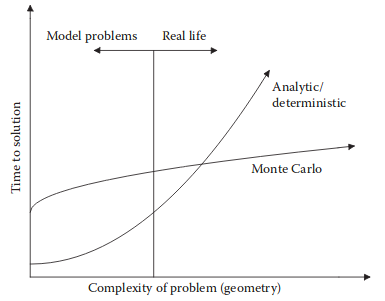
\includegraphics[scale=0.66]{Grafici/monte_carlo_vs_analytic2.png}
	\caption{Confronto fra il tempo necessario per la risoluzione di un problema con un metodo analitico-deterministico e con un metodo Monte Carlo, al variare della complessità del problema. Figura tratta da~\cite{bielajew:13}.} \label{fig:monte_carlo}
\end{figure}


%Nel campo della fisica, i metodi Monte Carlo sono spesso utilizzati per 
%Un notevole impulso allo sviluppo dei metodi Monte Carlo è provenuto dalla fisica delle alte energie, in cui l'elevata complessità degli apparati di rivelazione necessitava di uno strumento per decidere le specifiche in fase di progettazione.


%Un notevole impulso allo sviluppo dei metodi Monte Carlo è provenuto dalla fisica delle alte energie, in cui la crescente necessità di simulare complessi sistemi di rivelazione spingeva per la realizzazione di software sempre più performanti e robusti.
%
% ***** PRIMA AVEVO MESSO QUESTA
%Un notevole impulso allo sviluppo dei metodi Monte Carlo è provenuto dalla fisica delle alte energie, in cui si comprese che tali metodi offrivano la possibilità di seguire la traccia delle particelle e simulare le loro interazioni con la materia.
%
Un notevole impulso allo sviluppo delle tecniche di simulazione è provenuto dalla fisica delle alte energie, in cui si comprese che tali strumenti, offrendo la possibilità di seguire le tracce delle particelle ed ``imitare'' le loro interazioni con la materia, potevano essere impiegati sia per la progettazione dei rivelatori sia per lo studio della loro risposta nelle condizioni sperimentali di interesse.
In questo contesto nacque il codice \emph{GEANT}, di cui nella sezione successiva si espongono le principali caratteristiche.





%\section{\iflanguage{italian}{La piattaforma \textsc{Geant4}}{\textsc{Geant4} toolkit}}

\section{\iflanguage{italian}{La piattaforma Geant4}{Geant4 toolkit}}

%\section{\textsc{Geant4}}

La piattaforma GEANT, il cui nome deriva da \emph{GEometry ANd Tracking}, fu sviluppata nel 1974 al CERN di Ginevra allo scopo di simulare l'interazione di particelle elementari ad alta energia con i rivelatori.
%Questa prima versione consentiva di simulare il trasporto di un numero ristretto di particelle 
%In questa prima versione era possibile simulare soltanto un numero ristretto di particelle
In questa prima versione era possibile considerare soltanto un numero ristretto di particelle e forme geometriche semplici. 
Nel 1982 venne distribuito GEANT3, scritto in FORTRAN e nettamente potenziato rispetto al suo predecessore; infatti, si potevano simulare apparati sperimentali grandi e sofisticati e fasci di particelle molto energetici.
Tuttavia, il codice presentava una struttura molto complessa, che rendeva difficile l'introduzione di nuove caratteristiche o la ricerca di errori.
%the simulation software geant4, which means \emph{geometry and tracking}, is a toolkit based on
%Fu così che si arrivò al 1998, anno dell'uscita dell'ultima versione del codice, chiamata \geant, interamente basata sul linguaggio C++.
%La crescente necessità di simulare complessi sistemi di rivelazione spingeva per la realizzazione di software sempre più performanti e robusti.
%
%%Fu così che nel 1998, grazie alla collaborazione di oltre 40 istituti internazionali, venne pubblicata l'ultima versione del codice, chiamata \geant.
D'altro canto, la crescente necessità di simulare complessi sistemi di rivelazione spingeva per la realizzazione di software sempre più performanti e robusti.
Fu così che nel 1998, grazie alla collaborazione di oltre 40~istituti internazionali, venne pubblicato un nuovo progetto, chiamato~\geant.
Esso è interamente basato sul linguaggio C++, traendo vantaggio, dunque, da tutte le potenzialità offerte da una tecnologia orientata agli oggetti, come ad esempio la modularità e la compattezza.
% oppure il polimorfismo
%Il modo più corretto di definire \geant{} è \emph{toolkit}, ovvero ``cassetta per gli attrezzi'', in quanto comprende un insieme di librerie software che l'utente può selezionare a seconda delle proprie esigenze per creare un'applicazione specifica.

Oggi \geant{} consente di simulare l'interazione con la materia di tutte le particelle note, in un range energetico che va da pochi~eV fino ai~TeV.
%
%La sua notevole duttilità lo ha reso uno strumento 
Grazie alla sua notevole duttilità, sono innumerevoli gli esperimenti che si avvalgono di questo strumento: la sua area d'azione comprende la fisica delle alte energie, la fisica nucleare, le applicazioni in campo medico e l'astrofisica.
Il codice è, inoltre, open-source e viene periodicamente aggiornato dalla collaborazione. 
Dal momento che la documentazione su \geant{} è ampia e dettagliata\footnote{Si veda, ad esempio, \url{www.geant4.org}.}, nel prosieguo vengono presentati soltanto gli aspetti utili alla comprensione delle simulazioni svolte per questo lavoro di tesi.  



%\subsection{\iflanguage{italian}{La struttura di \textsc{Geant4}}{\textsc{Geant4} structure}}

\subsection{\iflanguage{italian}{La struttura di Geant4}{Geant4 structure}}

%Il modo più corretto di definire \geant{} è \emph{toolkit}, ovvero ``cassetta per gli attrezzi'', in quanto comprende un insieme di librerie software che l'utente può selezionare a seconda delle proprie esigenze per creare un'applicazione specifica.
Il modo più corretto di definire \geant{} è \emph{toolkit}, ovvero ``cassetta per gli attrezzi'', in quanto è costituito da un insieme di librerie software che, a seconda delle esigenze, possono essere selezionate per creare un'applicazione specifica.
L'utente deve, quindi, scrivere la sua applicazione, definendo tutti i parametri rilevanti: alcuni devono essere inseriti in modo obbligatorio, altri possono essere aggiunti facoltativamente.
%\geant{} offre numerose funzionalità:

%Ogni simulazione si compone dei seguenti aspetti: 
Nella progettazione e nella realizzazione del software, tutti gli aspetti fondamentali di un processo di simulazione sono stati inclusi:
\begin{itemize}
	\item la geometria del sistema, specificando forma, dimensione e posizione dei vari oggetti;
	\item i materiali utilizzati;
	\item la sorgente delle particelle, di cui si definisce la posizione, l'energia, la distribuzione angolare e tutte le altre caratteristiche rilevanti;
	\item i processi fisici di interazione per la modellizzazione  del comportamento delle particelle;
	%\item il tracciamento delle particelle, che può essere calcolato anche passo dopo passo, consentendo di estrarre ad ogni step informazioni legate alla particella, come ad esempio energia e posizione;
	\item il tracciamento delle particelle attraverso materiali ed, eventualmente, campi elettromagnetici esterni;
	%\item la sensitività di un rivelatore e la sua risposta;
	\item la definizione di elementi sensibili, che simulano la risposta del rivelatore;
	\item la visualizzazione tridimensionale degli oggetti simulati e delle tracce delle particelle;
	\item la generazione di dati, i quali possono essere memorizzati per una successiva analisi.
\end{itemize}


%Ciascuno degli aspetti elencati corrisponde ad una determinata \emph{classe} o \emph{categoria}, che, agendo in modo indipendente l'una dall'altra, danno al software una struttura modulare.

Gli aspetti elencati corrispondono in \geant{} a determinate \emph{classi} o \emph{categorie}, che, agendo in modo indipendente l'una dall'altra, danno al software una struttura modulare.
%Esse sono state concepite per essere facilmente estendibili o modificabili dall'utente, seguendo la logica tipica dei linguaggi orientati agli oggetti;
Esse sono state concepite per essere facilmente estendibili o modificabili, seguendo la logica tipica dei linguaggi orientati agli oggetti; infatti, grazie ad un approccio basato sul \emph{polimorfismo} e sull'\emph{ereditarietà}, l'utente può fornire un'implementazione alternativa delle funzioni presenti in una categoria.
%Esse sono state concepite per essere facilmente estendibili o modificabili, seguendo la logica tipica dei linguaggi orientati agli oggetti; \geant{} usa, infatti, un approccio basato sulle proprietà del \emph{polimorfismo} e dell'\emph{ereditarietà}.
%Di tutte le classi messe a disposizione, \geant{} richiede obbligatoriamente l'implementazione e l'istanziazione di tre, ovvero 
%\geant mette a disposizione un grande numero di classi, le quali sono state  concepite per essere facilmente estendibili o modificabili dall'utente, seguendo la logica tipica dei linguaggi orientati agli oggetti.
%L'implementazione e l'istanziazione di queste classi sono obbligatorie in tre casi, ovvero
%\geant{} mette a disposizione un grande numero di classi, ma per tre di loro l'implementazione e l'istanziazione sono obbligatorie.
\geant{} mette a disposizione un grande numero di classi, richiedendo obbligatoriamente l'implementazione e l'istanziazione per tre di loro: 
\begin{itemize}
	\item la classe dedicata alla definizione della geometria e dei materiali;
	\item la classe prevista per la definizione delle particelle, dei processi fisici e delle soglie per la produzione dei secondari;
	\item la classe rivolta alla generazione delle particelle primarie.
\end{itemize}


%Altre classi

Le altre classi sono, invece, opzionali e, a seconda delle esigenze, l'utente può modificarne il comportamento di default definendo la propria ``versione''; 
%ad esempio, ai fini di questo lavoro è stato necessario personalizzare la classe che rappresenta ogni ``passo'' della traccia della particella, facendo in modo che ad ogni step venisse estratta l'informazione sulla perdita di energia e sulla posizione.
%
ad esempio, in \geant{} esiste una classe che rappresenta ogni ``passo'' (più propriamente chiamato \emph{step}) della traccia di una particella, sia essa primaria o secondaria.
%, laddove per passo possiamo immaginare un segmento che compone la traiettoria.
L'utente può personalizzare la funzione che accede alle informazioni dello step (chiamata \emph{UserSteppingAction}), facendo in modo che ad ogni step vengano, ad esempio, estratte la posizione e l'energia della particella.
%In \geant{} la traccia della particella è divisa in \emph{step}, che, per comodità, possiamo immaginare come dei segmenti.
%Grazie ad un'apposita classe, è possibile accedere a diverse informazioni legate a tale step, come estremi 


\section{\iflanguage{italian}{Gli aspetti principali della simulazione}{Simulation main aspects}}

%La simulazione implementata per questo lavoro di tesi considera una matrice di telescopi SiC-CsI.
%Allo scopo di valutare le prestazioni di PID
Nell'ambito di questo lavoro di tesi è stata realizzata un'applicazione in \geant{} per simulare la risposta di un sistema di telescopi SiC-CsI agli ioni di interesse per il progetto NUMEN.
Nel seguito di questa sezione vengono illustrate nel dettaglio le caratteristiche di tale applicazione.




\subsection{\iflanguage{italian}{La geometria e i materiali}{Geometry and materials}} \label{par:geometria}

Ciascun telescopio è formato da due stadi, il rivelatore al carburo di silicio (SiC) e il cristallo allo ioduro di cesio (CsI), i quali sono posti a contatto.
Per tenere in considerazione il substrato morto del rivelatore al SiC, il primo stadio è, a sua volta, costituito da due parti: il volume attivo e il substrato morto.

Considerando un sistema di riferimento in cui l'asse $z$ è individuato dalla direzione di propagazione delle particelle, i telescopi sono fra loro separati di 2~mm lungo la direzione $x$ e di 1~mm lungo la direzione $y$.

%Ciascun telescopio è formato da tre parti: il volume attivo del rivelatore al SiC, il substrato morto dello stesso rivelatore e il cristallo allo CsI.

%In accordo con le 
%
%Un importante aspetto della simulazione riguarda lo spessore dei rivelatori.


%Dal momento che nuovi sviluppi tecnologici hanno reso possibile la rimozione quasi totale del substrato, sono state svolte anche delle simulazioni in cui il suo spessore era ridotto a 10~$\mu$m. 
%Per quanto riguarda il cristallo di CsI, lo spessore è stato posto uguale a 1~cm.


%Poiché uno degli obiettivi di questo lavoro consisteva nella ricerca delle migliori condizioni di granularità,  sono stati considerati diversi valori per le dimensioni trasversali; in particolare, sulla base degli attuali limiti imposti dal processo di produzione dei rivelatori al SiC, sono state simulate aree sensibili di $1 \times 1$, $1.5 \times 1.5$ e $2 \times 2$~cm\ap{2}.
%Poiché uno degli obiettivi di questo lavoro consisteva nella ricerca delle migliori condizioni di granularità,  per le dimensioni trasversali dei telescopi sono stati presi in esame diversi valori; in particolare, sulla base degli attuali limiti imposti dal processo di produzione dei rivelatori al SiC, sono state simulate aree sensibili di $1 \times 1$, $1.5 \times 1.5$ e $2 \times 2$~cm\ap{2}.
Poiché uno degli obiettivi principali di questo lavoro consisteva nella ricerca delle condizioni ottimali di granularità, sono state condotte diverse simulazioni al variare delle dimensioni trasversali dei telescopi; in particolare, sulla base degli attuali limiti imposti dal processo di produzione dei rivelatori al SiC, sono state simulate aree sensibili di $1 \times 1$, $1.5 \times 1.5$ e $2 \times 2$~cm\ap{2}.




%Lo spessore del primo è di 100~$\mu$m, mentre quello del secondo è di 350~$\mu$m.
%Un altro aspetto importante della simulazione riguarda lo spessore del rivelatore al SiC; infatti, sebbene la collaborazione abbia suggerito 
%Per quanto riguarda lo spessore dei due stadi del telescopio, la collaborazione aveva individuato come probabile soluzione l'utilizzo di rivelatori al SiC da 100~$\mu$m e di cristalli allo CsI di 1~cm. 

%Lo standard tecnologico attuale prevede che un rivelatore al SiC di tale spessore abbia un substrato morto spesso 350~$\mu$m.
Per quanto riguarda lo spessore dei due stadi del telescopio, in accordo con la soluzione individuata dalla collaborazione, sono stati simulati rivelatori al~SiC da 100~$\mu$m e cristalli allo CsI da 1~cm, mentre per il substrato morto si è considerato un valore di 350~$\mu$m.
%Gli spessori tenuti in considerazione erano di 100~$\mu$m per il rivelatore al SiC, di 350~$\mu$m per il substrato morto e di 1~cm per il cristallo allo CsI.
Tuttavia, dal momento che nuovi sviluppi tecnologici hanno reso possibile la rimozione quasi totale degli strati morti, si è esaminato anche il caso in cui lo spessore del substrato fosse ridotto a 10~$\mu$m. 
È stato, dunque, effettuato un confronto tra le diverse condizioni, al fine di valutarne le conseguenze sulle capacità di~PID.





%Sebbene il muro di telescopi comprenderà oltre 1000 
%La simulazione ha considerato un unico modulo di $2 \times 5$ rivelatore.

%%Dal momento che per gli scopi di questo lavoro non era necessario includere l'intero muro di 1230 telescopi, tutte le simulazioni sono state svolte prendendo in esame una matrice di $2 \times 5$ elementi.

In Figura~\ref{fig:simulazione_muro} è mostrato l'aspetto assunto da un modulo elementare di~$2 \times 5$ telescopi nella simulazione \geant. 
Dal momento che allo scopo di valutare le capacità di PID del sistema non è necessario includere l'intero muro di rivelatori, tutte le simulazioni sono state svolte considerando un solo telescopio.
%In Figura~ è possibile vedere la realizzazione grafica di \geant{} di un modulo $2 \times 5$ del sistema di rivelazione.

\begin{figure} [!p]
	\centering
	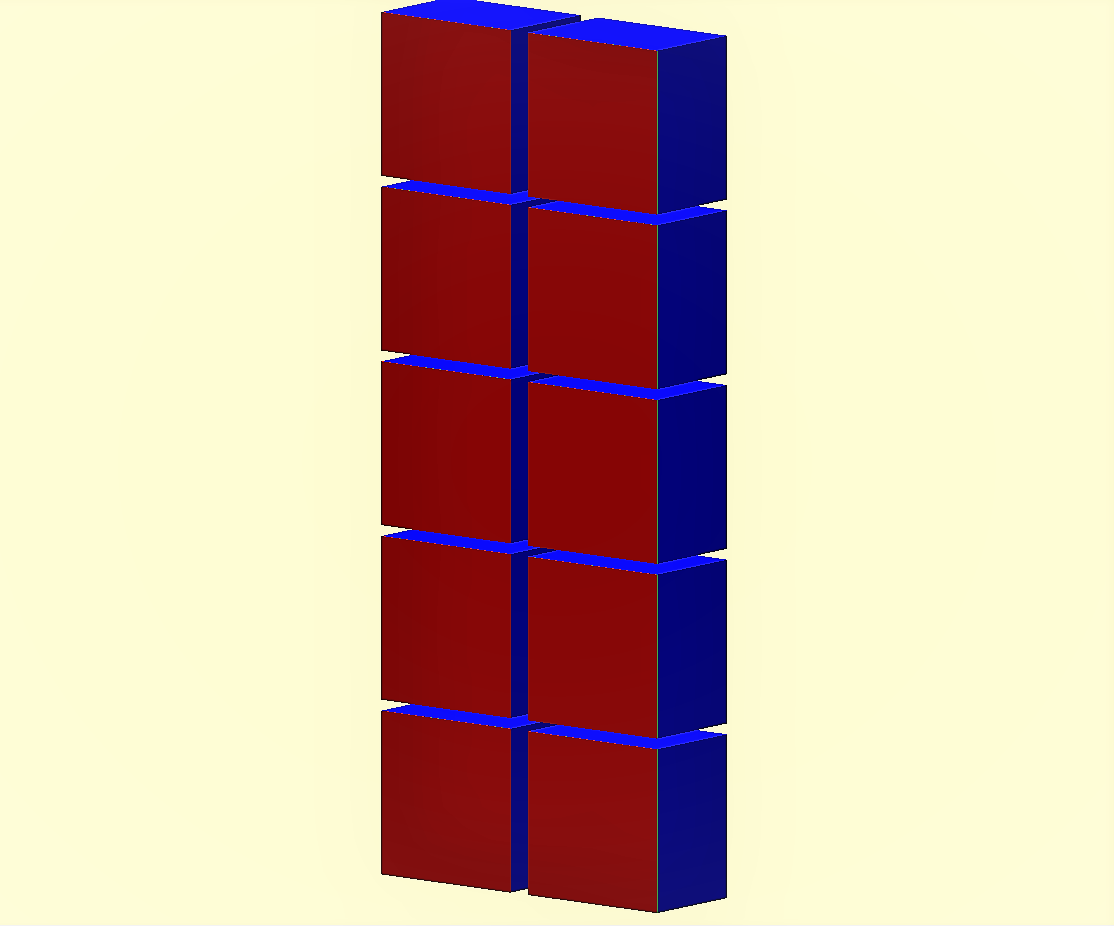
\includegraphics[width=\textwidth, keepaspectratio]{Grafici/modulo2_ritagliato.png}
	\caption{Una matrice di $2 \times 5$ telescopi: in rosso il rivelatore al SiC, in verde, appena visibile, il substrato morto di tale rivelatore e in blu il cristallo allo CsI.} \label{fig:simulazione_muro}
\end{figure}


\subsection{\iflanguage{italian}{La generazione delle particelle primarie}{Primary particles generation}} \label{par:particelle_primarie}

%Le particelle primarie simulate comprendono tre degli ioni di maggiore interesse per NUMEN, ovvero \ce{^{18}O}, \ce{^{18}F} e \ce{^{18}Ne}. 
%In alcune simulazioni sono stati coinvolti anche altri isotopi di tali specie nucleari, 
%Le particelle primarie simulate comprendono tre degli ioni di maggiore interesse per NUMEN, ovvero \ce{^{18}O}, \ce{^{18}F} e \ce{^{18}Ne}, coinvolgendo in alcune simulazioni anche altri isotopi di tali specie atomiche, quali \ce{^{16}O}, \ce{^{17}O}, \ce{^{19}F}, \ce{^{20}F}, \ce{^{19}Ne} e \ce{^{20}Ne}.
In una simulazione \geant{} i parametri che tipicamente devono essere introdotti per la generazione di un evento sono: la tipologia della particella primaria, la sua energia cinetica iniziale, la sua direzione iniziale e la sua posizione iniziale.
%In questo paragrafo verranno spiegate le condizioni di lavoro scelte in merito a tali parametri.
In questo paragrafo verranno spiegate le scelte effettuate in merito a tali parametri.
%(\textcolor{red}{Lo tolgo questo paragrafetto?})

Le particelle primarie simulate comprendono nove degli ioni di maggiore interesse per NUMEN, ovvero \ce{^{18}O}, \ce{^{19}O}, \ce{^{20}O}, \ce{^{18}F}, \ce{^{19}F}, \ce{^{20}F}, \ce{^{18}Ne}, \ce{^{19}Ne} e~\ce{^{20}Ne}.
In alcuni casi esaminati gli ioni sono stati considerati completamente ionizzati, mentre in altri sono stati simulati diversi stati di carica.

%In ciascun evento, la particella primaria è stata generata in modo casuale sulla faccia anteriore del rivelatore al SiC centrale, con una direzione estratta casualmente all'interno di un angolo solido corrispondente ad un cono con un'apertura di~20\textdegree{}. 
%Poiché il sistema che si intende analizzare è posto nel piano focale di uno spettrometro magnetico, l'energia e la 
%Affinché gli eventi simulati potessero riprodurre fedelmente gli eventi reali, 
%al fine di riprodurre fedelmente gli eventi reali

%Poiché il sistema che si intende analizzare è posto nel piano focale di uno spettrometro magnetico, è stato necessario introdurre una correlazione tra la posizione di impatto delle particelle sul telescopio e la loro energia cinetica; infatti, nella situazione reale gli eiettili prodotti nell'interazione fra il fascio di particelle e il bersaglio attraversano il quadrupolo e il dipolo 

%Per quanto riguarda l'energia iniziale delle particelle primarie, bisogna ricordare che 


%Poiché il sistema che si intende analizzare sarà posto nel piano focale di uno spettrometro magnetico, l'energia delle particelle primarie deve essere correlata alla loro posizione di arrivo sul piano focale; infatti, nell'apparato sperimentale reale, gli eiettili, attraversando il dipolo, subiranno una deflessione dovuta alla forza di Lorentz. 

% la forza di Lorentz stabilisce la relazione 
%la quale definisce la traiettoria della particella fissandone il raggio di curvatura $\rho$.

%Poiché il sistema che si intende analizzare sarà posto nel piano focale di uno spettrometro magnetico, è stato necessario introdurre una correlazione tra la posizione di arrivo delle particelle sul piano focale e la loro energia cinetica; 
%Poiché il sistema che si intende analizzare sarà posto nel piano focale di uno spettrometro magnetico, l'energia cinetica delle particelle simulate non può essere indipendente dalla loro posizione di arrivo sul piano focale, ma deve essere introdotta una correlazione fra queste quantità;
Le energie cinetiche simulate devono essere scelte tenendo in considerazione che negli spettrometri magnetici gli ioni vengono separati in base alla loro \emph{rigidità magnetica} $B \rho$; infatti, quando una particella con carica~$q$ e massa $m$ si muove in un campo magnetico~$B$ ortogonale al suo impulso~$p$, a causa della forza di Lorentz essa descrive una traiettoria con raggio di curvatura~$\rho$, dato dalla nota relazione
\begin{equation} \label{eq:legge_spettrometri}
B  \rho \, = \,  \frac{p}{q}
\end{equation}
%In approssimazione non relativistica, l'impulso $p$ è legato all'energia cinetica $E$ dalla relazione $p = \sqrt{2 m E}$, laddove $m$ indica massa della particella; dunque, la precedente può essere scritta nella forma
%\begin{equation} \label{eq:legge_spettrometri_energia}
% \rho \, \propto \,  \frac{\sqrt{m}}{q} \sqrt{E}
%\end{equation}
%La~\ref{eq:legge_spettrometri_energia} afferma che 
Al primo ordine di approssimazione, $\rho$ è proporzionale a $x_{foc}$, coordinata orizzontale del punto di arrivo della particella sul piano focale.
Inoltre, in approssimazione non relativistica, l'impulso $p$ è legato all'energia cinetica $E$ dalla formula $p = \sqrt{2 m E}$. 
Esiste, dunque, una relazione fra $x_{foc}$ ed $E$: essa è circa quadratica e dipende dal rapporto $\sqrt{m}/q$, ovvero
\begin{equation} \label{eq:legge_spettrometri_approx}
B \, x_{foc} \, \propto \,  \frac{\sqrt{m}}{q} \sqrt{E}
\end{equation}
%La~\ref{eq:legge_spettrometri_approx} afferma che ioni uguali, emessi ad angoli differenti con energie cinetiche uguali, giungono sullo stesso punto del piano focale; equivalentemente, ioni uguali, emessi allo stesso angolo con energie cinetiche differenti, giungono su punti diversi del piano focale.
La~\ref{eq:legge_spettrometri_approx} afferma che ioni con la stessa rigidità magnetica giungono sullo stesso punto del piano focale; equivalentemente, ioni con diversa rigidità magnetica giungono su punti diversi del piano focale.
Quanto appena detto è illustrato in Figura~\ref{fig:magnex_diverse_traiettorie}, la quale mostra una simulazione GEANT di MAGNEX per diverse traiettorie accettate dallo spettrometro.
\begin{figure} [!t]
	\centering
	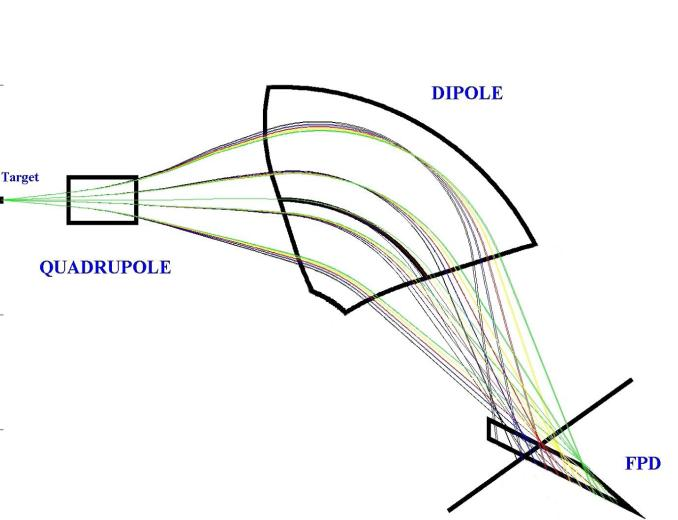
\includegraphics[width=\textwidth, keepaspectratio]{Grafici/magnex_traiettorie_diverse.png}
	\caption{Simulazione GEANT di MAGNEX: traiettorie con colori differenti hanno energie diverse. Figura tratta da~\cite{cappuzzello:epja16}.} \label{fig:magnex_diverse_traiettorie}
\end{figure}



A causa della estensione finita dei rivelatori, in realtà gli ioni arrivano sul telescopio in una finestra di valori di $B \rho$. La larghezza di tale finestra è data, al primo ordine, da
\begin{equation} \label{eq:finestra_Brho}
	\Delta \left(B \rho \right) \sim \frac{\Delta x}{D}
\end{equation} 
laddove $\Delta x$ indica l'estensione lungo la direzione dispersiva del rivelatore e $D$ è la dispersione in impulso dello spettrometro, pari a 3.68~cm/\%.

La dipendenza della \ref{eq:legge_spettrometri_approx} dal rapporto $\sqrt{m}/q$ costituisce il fondamento di un'innovativa tecnica di identificazione per spettrometri di grande accettanza; se, infatti, si misurano in correlazione la posizione $x_{foc}$ e l'energia cinetica~$E$, è possibile identificare gli ioni in massa e stato di carica.
L'applicazione di tale tecnica allo spettrometro MAGNEX è stata ampiamente discussa in numerose pubblicazioni, alle quali si rimanda per informazioni più dettagliate (si veda ad esempio~\cite{cappuzzello:nima10}). 

Dal momento che la simulazione deve riflettere il comportamento reale degli ioni nello spettrometro, è stato necessario introdurre le suddette correlazioni energia-posizione. 
Inoltre, nel meccanismo delle reazioni nucleari la cinematica introduce ulteriori correlazioni fra l'energia cinetica e l'angolo di emissione dell'eiettile.
Entrambi questi fattori sono caratterizzati da effetti non-lineari che difficilmente potevano essere inseriti direttamente nella simulazione \geant. 
%A tal fine si è scelto di utilizzare i software dedicati al trasporto ottico dei prodotti di reazione attraverso gli elementi magnetici dello spettrometro. 
Per questo motivo si è scelto di affidare l'introduzione di queste correlazioni a dei software già sviluppati e ottimizzati dalla collaborazione NUMEN.
%Poiché all'interno della collaborazione NUMEN erano già stati sviluppati e ottimizzati dei software dedicati al calcolo della cinematica di reazione e al trasporto ottico degli eiettili attraverso gli elementi magnetici dello spettrometro, si è scelto di   
Tali software sono basati sugli algoritmi di COSY INFINITY~\cite{makino:nima99} e utilizzano il formalismo dell'algebra differenziale per risolvere le equazioni del moto dei prodotti di reazione fino al decimo ordine~\cite{cappuzzello:epja16}.
Scegliendo la tipologia e l'energia della reazione nucleare di interesse, essi determinano la cinematica di reazione e lo spazio delle fasi iniziale; dopo di che calcolano la matrice del trasporto e ricostruiscono il moto degli eiettili fino all'ingresso del rivelatore di piano focale (Focal Plane Detector, FPD).
%Scegliendo lo spazio delle fasi iniziale, essi ricostruiscono il moto degli eiettili fino all'ingresso del rivelatore di piano focale (Focal Plane Detector, FPD), permettendo di conoscere alcune osservabili fondamentali, come l'energia cinetica~$E$, la posizione~$(x_{foc},y_{foc})$ e gli angoli~$(\theta_{foc},\phi_{foc})$ di incidenza. 
%Queste osservabili sono date in input alla simulazione \geant{}, la quale descrive dunque l'interazione degli ioni con il telescopio.
Questi software producono in output un file contenente i valori delle osservabili rilevanti, come ad esempio l'energia cinetica~$E$, la posizione~$(x_{foc},y_{foc})$ e gli angoli di incidenza~$(\theta_{foc},\phi_{foc})$ sul FPD.
La simulazione \geant{} è stata realizzata in modo da prendere in input tale file e, a partire da questo, ricavare tutte le informazioni necessarie per la generazione degli eventi; in altre parole, ad ogni particella primaria vengono assegnate un'energia cinetica iniziale, una posizione iniziale e una direzione iniziale lette dal file.
%I software per il trasporto tracciano gli ioni fino all'ingresso del FPD 
Rispetto all'ingresso del FPD, il telescopio è posto ad una distanza di 14~cm, in quanto nell'apparato sperimentale reale tale spazio è occupato dal tracciatore a~gas. 
Attualmente la simulazione non comprende tale rivelatore, per cui gli ioni percorrono un tratto nel vuoto.
L'integrazione tra i software dedicati al trasporto ottico e la simulazione \geant{} è stata fondamentale per riprodurre correttamente le condizioni operative reali dello spettrometro.

Per valutare le capacità di PID del telescopio era necessario che tutti gli ioni simulati andassero ad incidere sul dispositivo. 
In base a quanto detto precedentemente, essi devono dunque avere la stessa finestra di $B \rho$, che comporta energie cinetiche differenti per i diversi ioni. 
Fissato un valore di riferimento per la rigidità magnetica, grazie ai software per il trasporto è stato possibile determinare per ogni ione l'intervallo di energia cinetica corrispondente al range di $B \rho$ accettato dal telescopio.
%per ogni ione è stata determinata l'energia cinetica corrispondente a tale valore e 
%Fissato un valore di rigidità magnetica di riferimento, per ogni ione è stata determinata l'energia cinetica corrispondente a tale valore e, attorno a tale valore, è stato considerato un intervallo di energia cinetica di 10~MeV, in modo da coprire la 



%Per introdurre le correlazioni energia-posizione, si è scelto di utilizzare i software dedicati al trasporto ottico dei prodotti di reazione attraverso lo spettrometro magnetico. 


%Allo scopo di coprire un ampio range energetico, realisticamente significativo per NUMEN, le particelle primarie hanno un'energia scelta casualmente fra 500 e 1000~MeV.
%%Allo scopo di valutare la capacità di PID in un ampio range energetico, realisticamente significativo per NUMEN, sono state simulate particelle primarie con un'energia scelta casualmente fra 500 e 1000~MeV.
%Dal momento che l'apparato sperimentale si incardina sulle proprietà dello spettrometro magnetico MAGNEX, 

%%È bene ricordare che negli spettrometri magnetici la posizione di una particella al piano focale è correlata alla sua energia; infatti, partendo dalla nota relazione
%\begin{equation} 
%B  \rho \, = \,  \frac{p}{q} \, 
%\end{equation}
%laddove $B$ è il campo magnetico, mentre $\rho$, $p$ e $q$ sono, rispettivamente, il raggio di curvatura, l'impulso e la carica della particella, sotto opportune condizioni è possibile affermare che\footnote{La relazione $p = \sqrt{2 m E}$ vale in approssimazione non relativistica.}
%\begin{equation} 
%B x_{foc} \, \approx \, B  \rho  \, \propto \,  \frac{\sqrt{m}}{q} \sqrt{E_{resid}}
%\end{equation}
%Dunque, per tenere in considerazione questo aspetto, alcune simulazioni sono state svolte tenendo fissata la rigidità magnetica $B \rho$ degli ioni primari e variandone in corrispondenza l'energia.
%Inoltre, dal momento che negli spettrometri magnetici la posizione di una particella al piano focale è correlata alla sua energia, in accordo con la nota relazione
%\begin{equation} \label{eq:legge_spettrometri}
%B  \rho \, = \,  \frac{p}{q}
%\end{equation}
%laddove $B$ è il campo magnetico, mentre $\rho$, $p$ e $q$ sono, rispettivamente, il raggio di curvatura, l'impulso e la carica della particella, alcune simulazioni sono state svolte tenendo fissato la rigidità magnetica $B \rho$ degli ioni primari.



\subsection{\iflanguage{italian}{I processi fisici}{Physics processes}}


Affinché la simulazione possa riprodurre con la maggiore accuratezza possibile i risultati sperimentali reali, è di cruciale importanza la scelta dei processi fisici da considerare allo scopo di definire il comportamento delle particelle.
Per gli scopi di questo lavoro, in una prima fase sono state prese in esame soltanto le interazioni elettromagnetiche (oltre ai processi di decadimento e di decadimento radioattivo) in quanto sufficienti a separare i luoghi di specie atomiche diverse nelle matrici $\Delta E - E$.
Successivamente, sono state aggiunte anche le interazioni adroniche, incorporando, dunque, processi di scattering elastico e inelastico e meccanismi di reazioni nucleari.

In Figura~\ref{fig:simulazione_evento} è riportata la visualizzazione grafica della simulazione di 20~eventi nel caso in cui il modello dei processi fisici comprendesse sia le interazioni elettromagnetiche sia quelle adroniche: in nero sono raffigurate le tracce degli ioni primari, mentre in altri colori sono mostrate le tracce delle particelle secondarie originate da reazioni nucleari. 



\begin{figure} [!p]
	\centering
	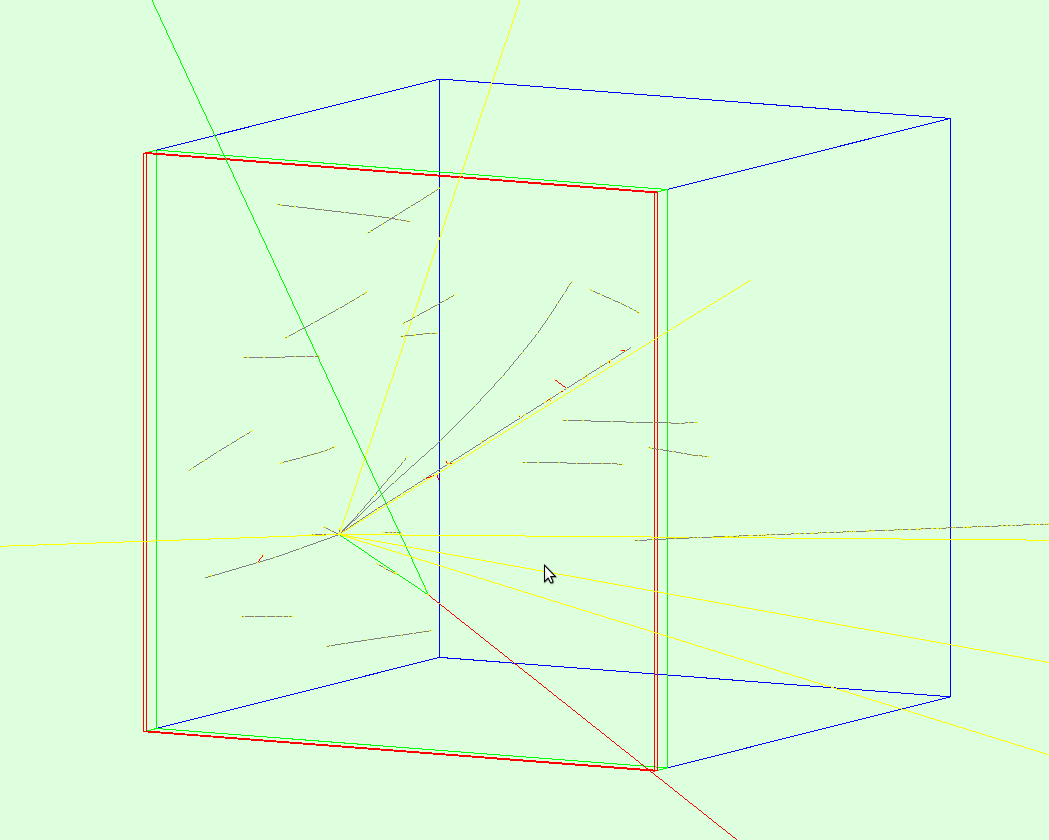
\includegraphics[width=\textwidth, keepaspectratio]{Grafici/evento5_ritagliato.png}
	\caption{Rappresentazione grafica della simulazione di 20~eventi: in nero le tracce degli ioni primari (\ce{^{18}O}), in altri colori le tracce delle particelle secondarie prodotte da reazioni nucleari con i nuclei del mezzo: dal momento che riescono ad uscire fuori dal rivelatore, si tratta, probabilmente, di particelle leggere, come protoni, neutroni e particelle $\alpha$.} \label{fig:simulazione_evento}
\end{figure}




%Non sono state modificate le impostazioni di default di
Una delle componenti fondamentali di \geant{} riguarda la scelta dei parametri di cut-off.
È possibile definire una soglia in range: elettroni di ionizzazione e gamma di bremsstrahlung aventi un range inferiore alla soglia non vengono generati esplicitamente, ma la loro energia viene considerata essere un deposito locale.
Dal momento che, ai fini di questo lavoro, una modifica dei parametri di cut-off non avrebbe portato a significativi cambiamenti dei risultati, si è scelto di mantenere le impostazioni di default, che corrispondono ad un range di 1~mm.



\subsection{\iflanguage{italian}{Tracciamento delle particelle}{Particles step}}

%In \geant{} la traccia della particella è divisa in \emph{step}, che, per comodità, possiamo immaginare come dei segmenti.
%Grazie ad un'apposita classe, è possibile accedere a diverse informazioni legate a tale step.
Come anticipato nella sezione precedente, in \geant{} è possibile modificare il comportamente della funzione UserSteppingAction.
Dal momento che, ai fini di questo lavoro, si volevano valutare le conseguenze sulla PID causate dagli effetti di bordo dei rivelatori, era necessario sapere punto per punto la posizione dello ione. 
Dunque, è stato modificato il comportamento di questa classe, affinché ad ogni step si conoscessero la posizione e il deposito di energia; in particolare, dal momento che \geant{} permette di conoscere gli estremi dello step, si è scelto di far corrispondere le coordinate del deposito di energia a quelle di un punto estratto in modo casuale sul segmento congiungente i due estremi.








\subsection{\iflanguage{italian}{Elaborazione post-simulazione}{Post-simulation processing}}

I dati prodotti dalla simulazione, scritti in un TTree di ROOT~\cite{brun:nima97}, sono stati elaborati da una macro di ROOT grazie alla quale sono state aggiunte alcune caratteristiche tipiche dei rivelatori reali e sono stati ricostruiti gli spettri energetici.
%In primo luogo, ciascun deposito di energia viene pesato con una funzione di r
%In primo luogo, dal momento che 
%
%In primo luogo, a causa del processo di produzione, i rivelatori al SiC presentano nel volume sensibile un bordo esterno completamente inattivo, dove la carica generata per ionizzazione non viene raccolta, ed una regione di transizione, in cui la carica prodotta viene raccolta soltanto in parte.
In primo luogo, a causa del processo di produzione, i rivelatori al SiC presentano attorno al volume sensibile un bordo esterno completamente inattivo ed una regione di transizione: nel primo la carica generata per ionizzazione non viene raccolta, nella seconda viene raccolta soltanto in parte.
Secondo le misurazioni effettuate, la zona totalmente morta ha una lunghezza di circa 200~$\mu$m, mentre la regione di transizione ha un'estensione di circa 50~$\mu$m. 
%Nella macro si è tenuto conto di tali \emph{effetti di bordo} pesando ciascun deposito di energia con una \emph{funzione di risposta} lineare, che nel caso unidimensionale sarebbe così definita: 
%\begin{equation}
%f(x) =
%\begin{cases}
%1        & \quad  x<a \\
%\alpha x & \quad  b<x<a\\
%0        & \quad  x>b
%\end{cases}
%\end{equation}
%
Nella macro si è tenuto conto degli \emph{effetti di bordo} pesando ciascun deposito di energia con una \emph{funzione di risposta} così definita: nella zona interamente attiva era pari ad uno, nella regione di transizione decresceva linearmente e nella zona del tutto inattiva aveva valore nullo.
Uno grafico esemplificativo dell'andamento di tale funzione nel caso unidimensionale è riportato in Figura~\ref{fig:funzione_risposta}.


\begin{figure} [!p]
	\centering
	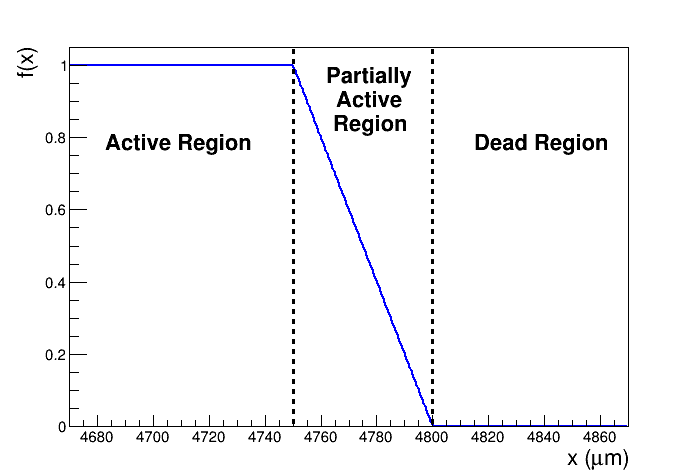
\includegraphics[width=\textwidth, keepaspectratio]{Grafici_Tesi/Funzione/funzione.png}
	\caption{L'andamento della funzione di risposta $f(x)$ assunta per descrivere gli effetti di bordo del rivelatore al SiC.} \label{fig:funzione_risposta}
\end{figure}

%Nella macro, inoltre, sommando le diverse perdite di energia, per ogni evento veniva ricostruito il deposito energetico totale nel rivelatore al SiC e nel cristallo allo CsI.
Nella macro, inoltre, sommando step dopo step l'energia persa dallo ione, per ogni evento è stata ricostruita l'energia rilasciata nel rivelatore al SiC e quella depositata nel cristallo allo CsI.
Registrando, evento per evento, tutti i depositi di energia, si sono riprodotti gli spettri energetici degli ioni per entrambi gli stadi del telescopio.
A questo livello, soltanto le fluttuazioni statistiche legate alla ionizzazione sono tenute in considerazione.
Dunque, al fine di riprodurre le risoluzioni energetiche tipiche dei rivelatori in esame, lo spettro energetico è stato ``allargato'' campionando ciascun deposito di energia con una distribuzione gaussiana, la cui espressione è
%\begin{equation}
%	f(E) = A \, \mbox{e}^{- \frac{E - E_0}{2 {\sigma}^2}}
%\end{equation}
\begin{equation}
	f(E, E_0, \sigma) = \frac{1}{\sqrt{2 \pi \sigma^2}} \, \exp \left[ - \frac{ \left(E - E_0 \right)^2}{2 {\sigma}^2}  \right]
\end{equation}
dove $E_0$ è il valore originario del deposito di energia, $E$ è il valore dopo il campionamento e $\sigma$ è la deviazione standard.
Di tale distribuzione, noto il valore medio $E_0$, bisognava scegliere la $\sigma$ in modo tale che la risoluzione energetica ricavata dalla simulazione fosse confrontabile con quella sperimentale.
%Dal momento che la risoluzione energetica è generalmente espressa come la somma in quadratura di un termine legato alle fluttuazioni statistiche del numero dei portatori e di uno dovuto al rumore elettronico, nella macro si è parametrizzata la $\sigma$ nel modo seguente
La risoluzione energetica è generalmente espressa come la somma in quadratura di un termine legato alle fluttuazioni statistiche del numero dei portatori, proporzionale a $E^{-1/2}$, e di uno dovuto al rumore elettronico, proporzionale a $E^{-1}$~\cite{knoll:10}.
Dunque, dal momento che la $\sigma$ può essere messa in relazione alla risoluzione energetica $R$ attraverso la~formula
\begin{equation}
	R \,  = \, \frac{\mbox{FWHM}}{E} \, = \, \frac{2.35 \, \sigma}{E}
\end{equation}
nella macro si è parametrizzata la deviazione standard nel modo seguente
\begin{equation}
\sigma = \sqrt{a + b \, E}
\end{equation}
laddove $a$ e $b$ sono due costanti.
%che assumono valori diversi a seconda che si consideri il rivelatore al SiC o il cristallo allo CsI. 
Nella somma al secondo membro, il primo addendo corrisponde al termine legato al rumore elettronico, mentre il secondo rappresenta quello causato dalle fluttuazioni del numero di portatori.
%
%
%Ricordando che la FWHM è legata alla $\sigma$ dalla relazione
%\begin{equation}
%\mbox{FWHM} = 2.35 \, \sigma
%\end{equation}
%la deviazione standard risulta collegata alla risoluzione energetica.
%Dal momento che quest'ultima è generalmente determinata dalla somma in quadratura di un termine legato all
Scegliendo opportuni valori per $a$ e $b$, si è assunta per il rivelatore al SiC una risoluzione energetica intrinseca dello 0.8\% FWHM a 25.3~MeV, mentre per il rivelatore allo CsI del 2\% FWHM a 700~MeV, in affinità con i valori tipici di questi dispositivi. 







%\clearpage


\section{\iflanguage{italian}{I risultati}{Results}}

In questa sezione vengono presentati i risultati ottenuti dalle simulazioni \geant{} del sistema di telescopi SiC-CsI.
Poiché l'obiettivo principale di questo lavoro di tesi consiste nella valutazione delle prestazioni di PID di tale sistema, la maggior parte delle simulazioni ha lo scopo di stimare la percentuale di errore che si avrebbe nell'identificazione degli ioni di interesse utilizzando la tecnica $\Delta E - E$.

È bene ricordare che tale tecnica prevede la correlazione fra la perdita di energia $\Delta E$ e l'energia cinetica totale $E$. In riferimento al caso in esame, $\Delta E$ corrisponde all'energia persa dalla particella primaria nel rivelatore al~SiC (che da ora in poi indicheremo con $ \Delta E_{SiC}$), mentre $E$ equivale alla sua energia cinetica iniziale. Nelle simulazioni svolte, quest'ultima quantità è data da
\begin{equation}
	E \, = \, \Delta E_{SiC} + E_{sub} + E_{CsI}
\end{equation}
laddove $E_{sub}$ è l'energia persa nel substrato morto ed $E_{CsI}$ è l'energia residua rilasciata nel cristallo allo CsI.
In realtà, $E_{sub}$ non sarebbe sperimentalmente accessibile; di conseguenza, per tenere conto delle energie realmente misurabili, bisogna introdurre la quantità $E_{meas}$, definita nel modo seguente
\begin{equation}
	E_{meas} \, = \, \Delta E_{SiC} + E_{CsI}
\end{equation}

%Dal momento che uno degli aspetti studiati in questo lavoro consiste nel valutare la differenza fra la correlazione $\Delta E - E_{tot}$ e quella $\Delta E - E_{resid}$, per maggiore chiarezza nel prosieguo verrà specificato se  
Inoltre, dal momento che uno degli aspetti studiati in questo lavoro consiste nel valutare se la correlazione $\Delta E_{SiC} - E_{CsI}$ può garantire prestazioni analoghe a quella $\Delta E_{SiC} - E_{meas}$, nel prosieguo verrà specificato quale tipo di correlazione si sta considerando.
%Dunque, dal momento che nel prosieguo verrà valutata la differenza fra le matrici 

%Per semplicità della trattazione si è preferito suddividere la sezione in paragrafi specifici, evidenziando di volta in volta quali parametri sono stati variati e quali sono stati tenuti fissi.
%Tenendo in mente questo obiettivo, per semplicità della trattazione si è preferito esporre i risultati evidenziando di volta in volta quali parametri sono stati variati e quali sono stati tenuti fissi.
Per semplicità della trattazione si è preferito esporre i risultati in modo schematico, evidenziando di volta in volta quali parametri sono stati variati e quali sono stati tenuti fissi.

%\subsection{\iflanguage{italian}{Caso ideale}{Ideal case}}
\subsection{\iflanguage{italian}{Particelle monocromatiche, ortogonali e centrali }{Monochromatic, orthogonal and central particles}}


Come primo esempio si è scelto di illustrare i risultati di un caso ideale in cui le particelle primarie sono generate con un'energia di 800~MeV ed incidono ortogonalmente e centralmente al telescopio, il quale ha, in questo caso, dimensioni trasversali di 1.5~cm $\times$ 1.5~cm.
%Il substrato epitassiale ha una lunghezza di 350~$\mu$m.
Per semplicità gli ioni considerati sono soltanto \ce{^{20}O}, \ce{^{20}F} e \ce{^{20}Ne}.
Nella prima fase di implementazione della simulazione, il modello dei processi fisici utilizzato prendeva in considerazione soltanto le interazioni elettromagnetiche, i processi di decadimento e di decadimento radioattivo.
Dal momento che la formula di Bethe-Bloch è ricavata tenendo conto della sola interazione elettromagnetica, il modello adottato è sufficiente a separare ioni diversi nelle matrici $\Delta E_{SiC} - E_{meas}$.
Questa affermazione viene confermata dalla Figura~\ref{fig:deltaE_ETot}, in cui è possibile notare che i luoghi di \ce{^{20}O}, \ce{^{20}F} e \ce{^{20}Ne} sono chiaramente distinti.
\begin{figure} [!t]
	\centering
	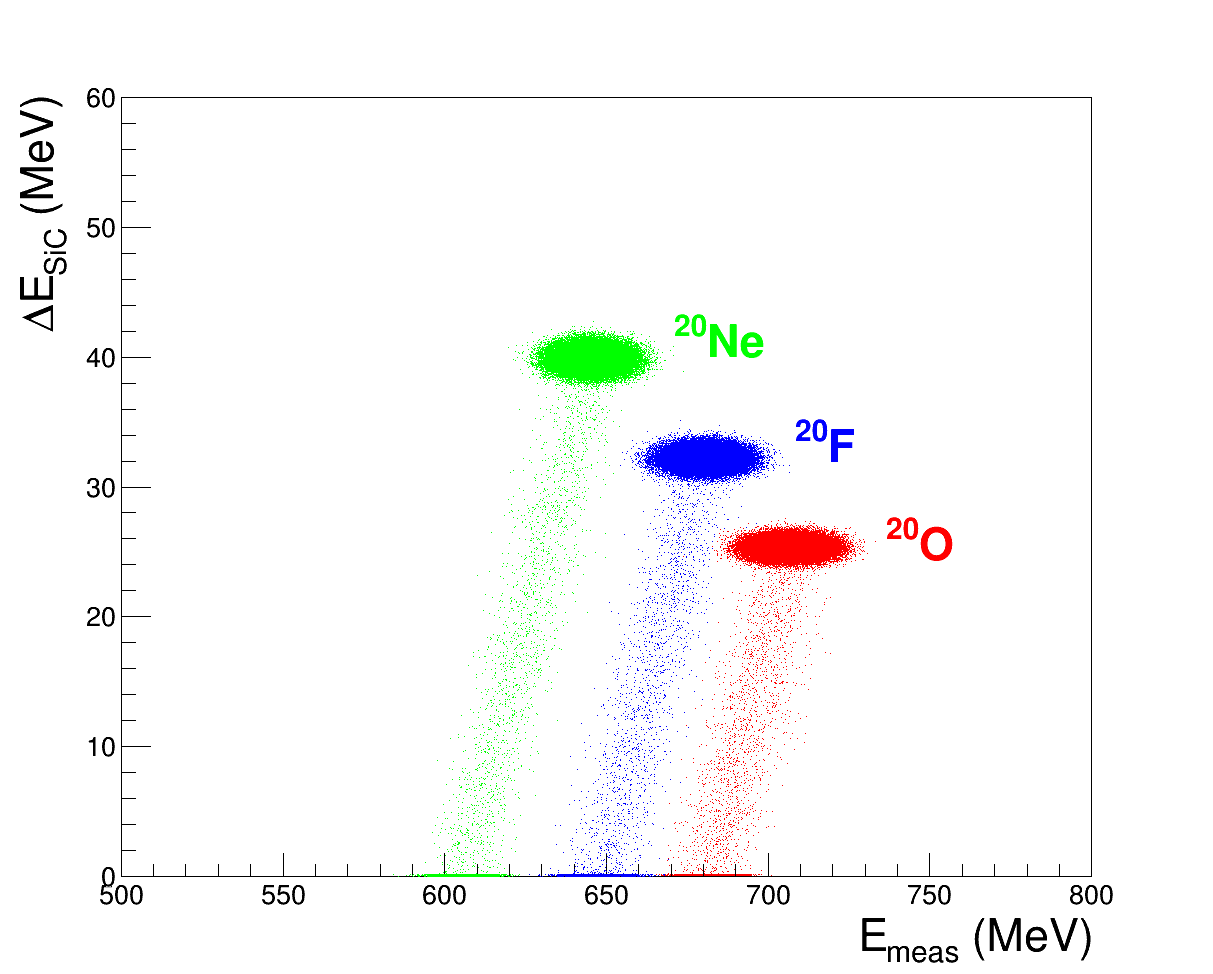
\includegraphics[width=\textwidth, keepaspectratio]{Grafici_Tesi2/Particelle_monocromatiche/deltaE_ETot_quadrata.png}
	\caption{Matrici $\Delta E_{SiC} - E_{meas}$ per \ce{^{20}O}, \ce{^{20}F} e \ce{^{20}Ne} con particelle monocromatiche, ortogonali e centrali.} \label{fig:deltaE_ETot}
\end{figure}
Sebbene si siano simulate particelle primarie monocromatiche, le matrici si dispongono ad $E_{meas}$ diverse perché la parte di energia persa nel substrato morto dipende dal numero atomico ($Z$) dello ione.
In secondo luogo, si fa notare che al di sotto di ciascuna delle tre matrici sono presenti degli eventi in cui l'energia residua è stata misurata correttamente, mentre la perdita di energia risulta inferiore al valore ``corretto'': si tratta di eventi in cui la carica prodotta nel rivelatore al SiC è stata raccolta parzialmente. 
Tali eventi costituiscono una delle principali componenti di errore nella PID, in quanto, potendo andare a posizionarsi sul luogo di uno ione diverso, in una procedura di identificazione effettuata mediante tagli grafici verrebbe attribuito loro uno~$Z$ errato.
Inoltre, essi costituiscono in ogni caso una perdita di segnali corretti che deve essere minimizzata, in particolar modo se si intende studiare processi estremamente rari come quelli di DCE.
Si deduce, quindi, che per avere delle buone capacità di PID è essenziale che la frazione di questi eventi rispetto al totale sia piccola.











In Figura~\ref{fig:deltaE_Tot} e in Figura~\ref{fig:ETot} sono riportate, rispettivamente, le proiezioni sull'asse $\Delta E_{SiC}$ e sull'asse $E_{meas}$ delle matrici $\Delta E_{SiC} - E_{meas}$: esse rappresentano gli spettri energetici misurati dal rivelatore al SiC e da quello allo~CsI.
Effettuando un fit gaussiano sul picco dell'\ce{^{20}O} nello spettro di $\Delta E_{SiC}$, si trova una FWHM di 1.1~MeV, corrispondente ad una risoluzione del 4.5\%.
Poiché questo valore è ben più grande della risoluzione intrinseca assunta per tale rivelatore, si deduce che in questo caso la componente più significativa della risoluzione compete alle fluttuazioni nel processo di ionizzazione.

\begin{figure} [!p]
	\centering
	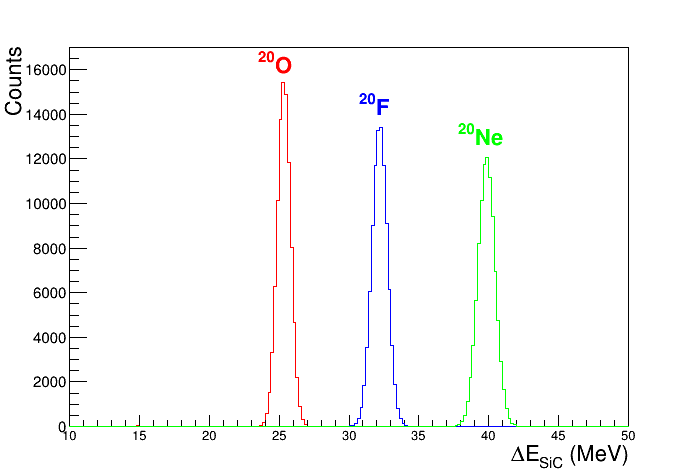
\includegraphics[scale=0.5]{Grafici_Tesi2/Particelle_monocromatiche/deltaE.png}
	\caption{Spettro in $ \Delta E_{SiC} $.} \label{fig:deltaE_Tot}
\end{figure}


\begin{figure} [!p]
	\centering
	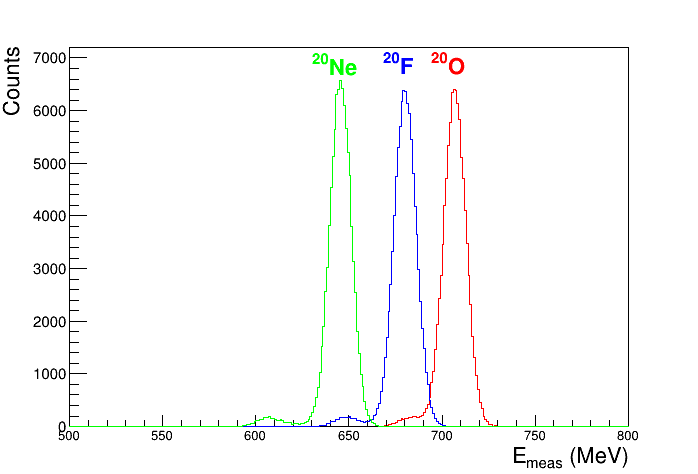
\includegraphics[scale=0.5]{Grafici_Tesi2/Particelle_monocromatiche/ETot.png}
	\caption{Spettro in $E_{meas} = \Delta E_{SiC} + E_{CsI}$.} \label{fig:ETot}
\end{figure}









%\subsection{\iflanguage{italian}{Processi fisici senza interazioni adroniche}{Physics process without adronic interactions}}
\subsection{\iflanguage{italian}{Particelle monocromatiche, non ortogonali e non centrali }{Not monochromatic, not orthogonal and not central particles}} \label{par:particelle_non_monocromatiche}







In questo secondo esempio ideale le particelle primarie hanno sempre un'energia di 800~MeV, ma la loro posizione iniziale è estratta casualmente sulla faccia anteriore del rivelatore al SiC centrale e la direzione del loro impulso varia in modo casuale in un cono di apertura di 20\textdegree{}.
Anche in questo caso viene utilizzato il modello dei processi fisici dell'esempio precedente, così come per la geometria e le dimensioni dei telescopi.
%La geometria e le dimensioni dei telescopi restano, invece, uguali a quelle dell'esempio precedente.
Le corrispondenti matrici $\Delta E_{SiC} - E_{meas}$ sono rappresentate in Figura~\ref{fig:deltaE_ETot_full_energy}.
%Inoltre, a differenza del caso precedente si nota la comparsa di eventi in cui la perdita di energia $\Delta E_{SiC}$ viene misurata correttamente, mentre l'energia $E_{tot}$ ha un valore inferiore rispetto a quello ``corretto''.
Rispetto al caso precedente, fanno la loro comparsa degli eventi in cui la perdita di energia $\Delta E_{SiC}$ viene misurata correttamente, mentre l'energia $E_{meas}$ ha un valore inferiore rispetto a quello corretto. 
Ciò dipende da quegli eventi in cui le particelle escono fuori dal cristallo allo CsI, non rilasciando totalmente la loro energia residua.
A causa del motivo precedentemente citato, anche questi eventi introducono una componente di errore nella PID e una perdita di segnali corretti.
\begin{figure} [!p]
	\centering
	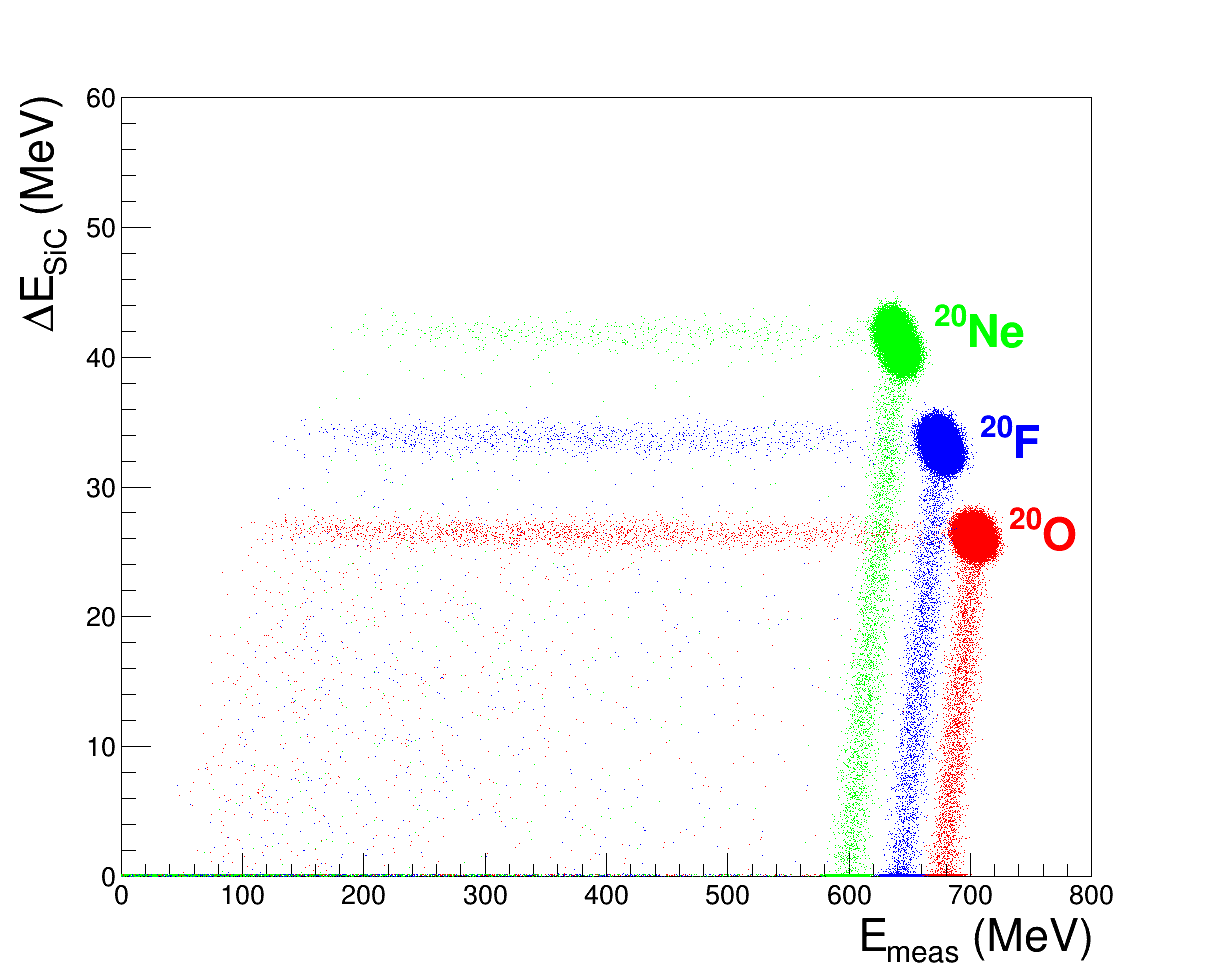
\includegraphics[width=\textwidth, keepaspectratio]{Grafici_Tesi2/Particelle_non_ortogonali/deltaE_ETot_intero_range_quadrata.png}
	\caption{Matrici $\Delta E_{SiC} - E_{meas}$ con particelle monocromatiche, non ortogonali e non centrali.} \label{fig:deltaE_ETot_full_energy}
\end{figure}
\begin{figure} [!p]
	\centering
	\subfigure[]
	{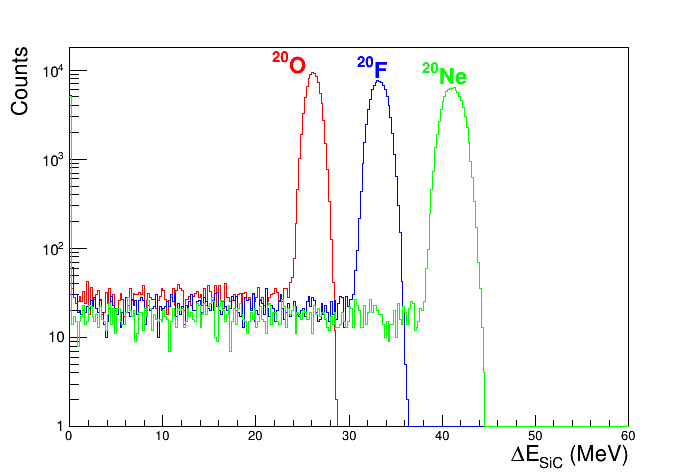
\includegraphics[scale=0.479]{Grafici_Tesi2/Particelle_non_ortogonali/deltaE.png}}
	%\vspace{7mm}
	\subfigure[]
	{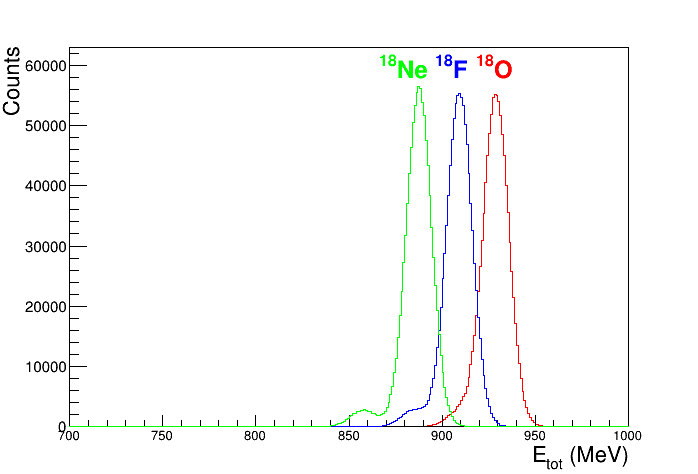
\includegraphics[scale=0.479]{Grafici_Tesi2/Particelle_non_ortogonali/ETot.png}}
	
	\caption{Le proiezioni delle matrici $\Delta E_{SiC} - E_{meas}$ di Figura~\ref{fig:deltaE_ETot_full_energy}: in (a) sull'asse $\Delta E_{SiC}$, in (b) sull'asse $E_{meas}$.} \label{fig:fetta}
\end{figure}
Per meglio comprendere l'entità degli eventi degradati, si sono riportate in Figura~\ref{fig:fetta} le proiezioni sull'asse verticale e su quello orizzontale della matrice: come si può notare, tali eventi costituiscono un continuo che si estende fino a zero e rendono asimmetriche le distribuzioni. 
In Figura~\ref{fig:fetta}.b si può, inoltre, osservare un secondo picco situato ad un valore di $E_{meas}$ di poco inferiore a quello assunto nel picco principale; esso è dovuto agli ioni che attraversano la cornice completamente inattiva attorno al rivelatore al~SiC, rilasciando una quantità di energia che non viene misurata.
%Allo scopo di dare una stima quantitativa della frazione di nuclei potenzialmente male identificati, il taglio per separare le differenti specie atomiche è stato scelto come il punto mediano fra due bande



%\begin{figure} [!p]
%	\centering
%	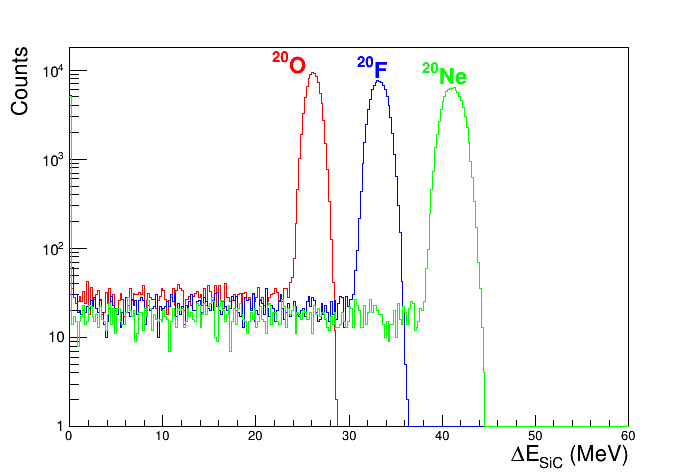
\includegraphics[scale=0.5]{Grafici_Tesi2/Particelle_non_ortogonali/deltaE.png}
%	\caption{Proiezione delle matrici di Figura~\ref{fig:fetta} sull'asse~$ E_{meas} $.} \label{fig:ETot1}
%\end{figure}


%\begin{figure} [!p]
%	\centering
%	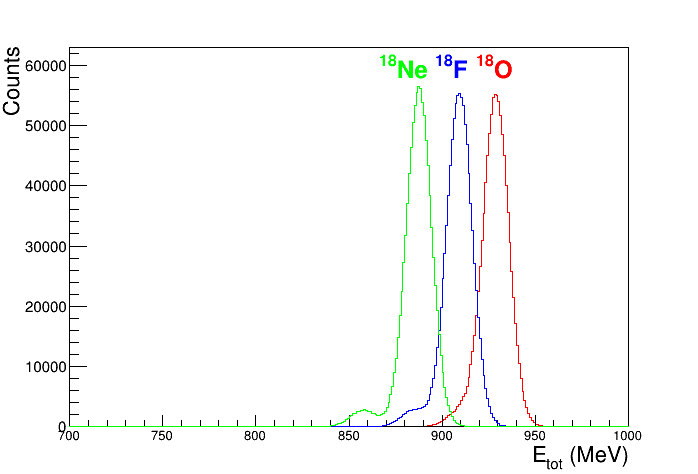
\includegraphics[scale=0.5]{Grafici_Tesi2/Particelle_non_ortogonali/ETot.png}
%	\caption{Proiezione delle matrici di Figura~\ref{fig:fetta} sull'asse~$ \Delta E_{SiC} $.} \label{fig:deltaE_Tot1}
%\end{figure}
%\begin{figure}[!p] 
%	\centering
%	\subfigure[]
%	{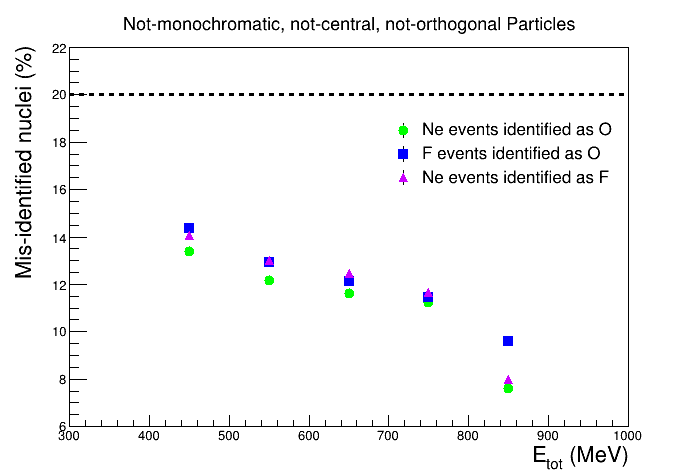
\includegraphics[scale=0.43]{Grafici_Tesi/Particelle_non_monocromatiche/leakage_alto_corr.png}}
%	\hspace{10mm}
%	\subfigure[]
%	{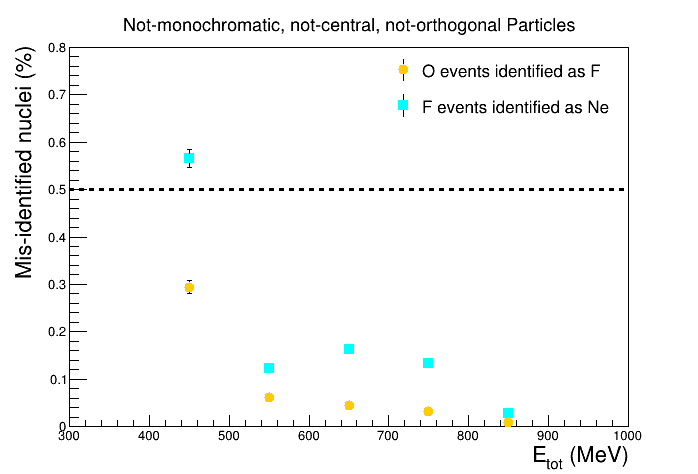
\includegraphics[scale=0.43]{Grafici_Tesi/Particelle_non_monocromatiche/leakage_basso_corr.png}}
%	\caption{La percentuale di nuclei identificati in modo erroneo in funzione di $E_{tot}$: in (a) la contaminazione da specie atomiche con $Z$ maggiore verso quelle con $Z$ minore, in (b) il viceversa. La linea tratteggiata in (a) indica il limite massimo imposto sul mancato riconoscimento del segnale, mentre in (b) rappresenta il limite massimo fissato sulla contaminazione del segnale. Laddove non sono mostrate, le barre di errore sono più piccole del marker.} \label{fig:leakage}
%\end{figure}

%\begin{figure} [!t]
%	\centering
%	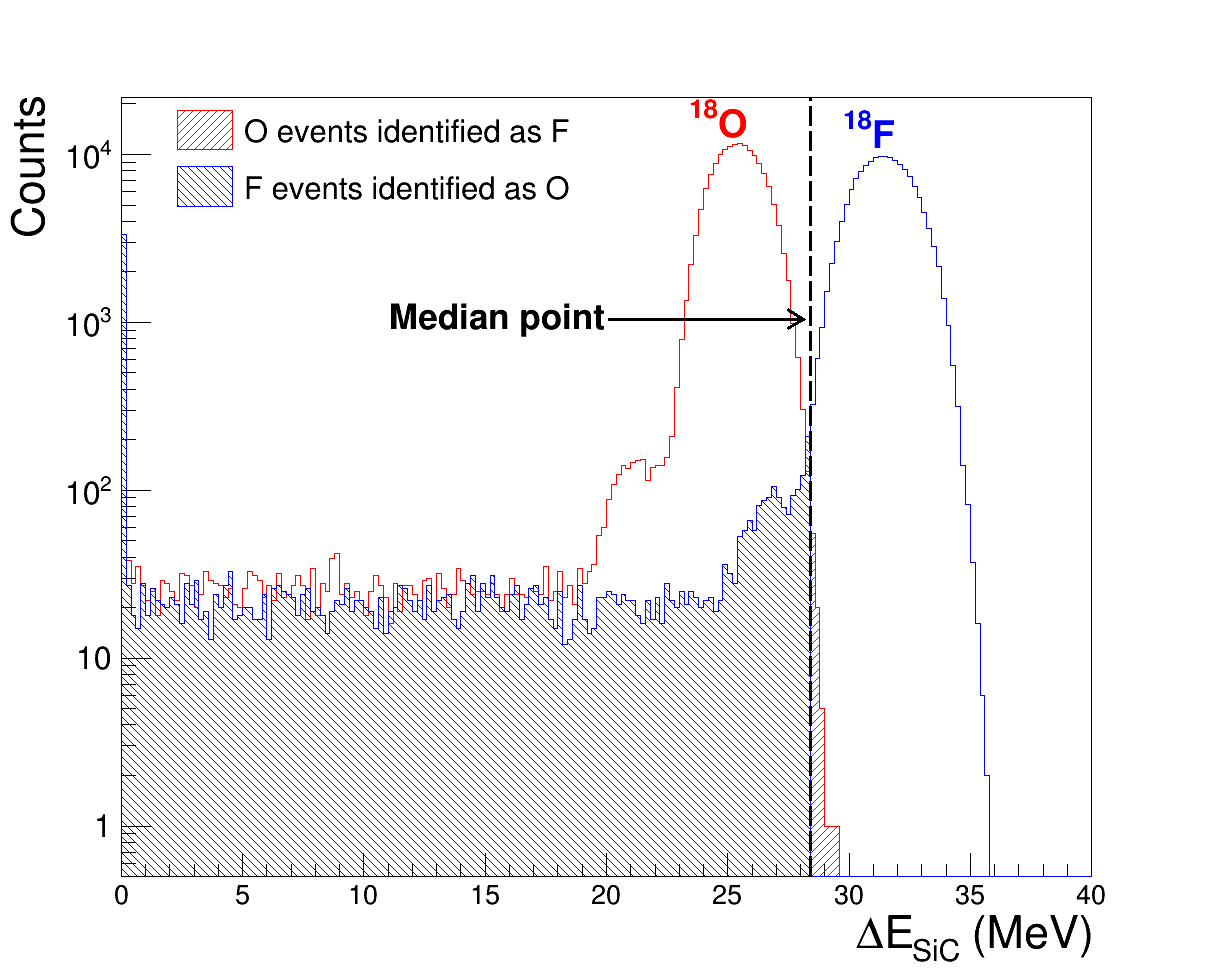
\includegraphics[scale=0.28]{Grafici_Tesi/Contaminazione/contaminazione.png}
%	\caption{Proiezione sull'asse $\Delta E_{SiC}$ della fetta in $E_{tot}$ compresa tra 600 e 700~MeV per l'\ce{^{18}O} e il \ce{^{18}F}. La linea tratteggiata indica il punto mediano tra i valori medi dei due spettri. In ombreggiatura blu si possono distinguere gli eventi di \ce{^{18}F} identificati come \ce{^{18}O}, in ombreggiatura rossa si notano gli eventi di \ce{^{18}O} identificati come \ce{^{18}F}.} \label{fig:fetta_con_contaminazione}
%\end{figure}










%%Allo scopo di dare una stima quantitativa della frazione di nuclei male identificati, si è proceduto nel modo seguente: si è diviso l'intero intervallo energetico $E_{tot}$ in un certo numero di fette; per ogni fetta si è effettuata una proiezione sull'asse $\Delta E_{SiC}$; per ogni coppia di specie atomiche si è calcolato il punto mediano fra i valori medi delle due distribuzioni; infine, si è determinato il numero di eventi al di sotto (o al di sopra) del punto mediano.
%%Un'immagine esemplificativa dell'idea alla base della procedura seguita è riportata in Figura~\ref{fig:fetta_con_contaminazione}: la linea tratteggiata indica il punto mediano tra i valori medi degli spettri di \ce{^{18}O} e \ce{^{18}F}.
%%A sinistra di tale punto sono evidenziati con ombreggiatura blu gli eventi di \ce{^{18}F} identificati come \ce{^{18}O}, mentre a destra sono contrassegnati con ombreggiatura rossa gli eventi di \ce{^{18}O} identificati come \ce{^{18}F}.
%%La contaminazione di \ce{^{18}F} in \ce{^{18}O} può essere, dunque, calcolata integrando lo spettro del \ce{^{18}F} da zero fino al punto mediano; invece, la contaminazione di \ce{^{18}O} in \ce{^{18}F} viene determinata integrando lo spettro dell'\ce{^{18}O} dal punto mediano fino alla fine della distribuzione.
%%La scelta del punto mediano come soglia è arbitraria e non necessariamente ottimale: è funzionale comunque per fare un confronto quantitativo e omogeneo fra molte configurazioni diverse.
%per quantificare la contaminazione di \ce{^{18}O} in \ce{^{18}F} si calcola 

%\begin{figure}[!p] 
%	\centering
%	\subfigure[]
%	{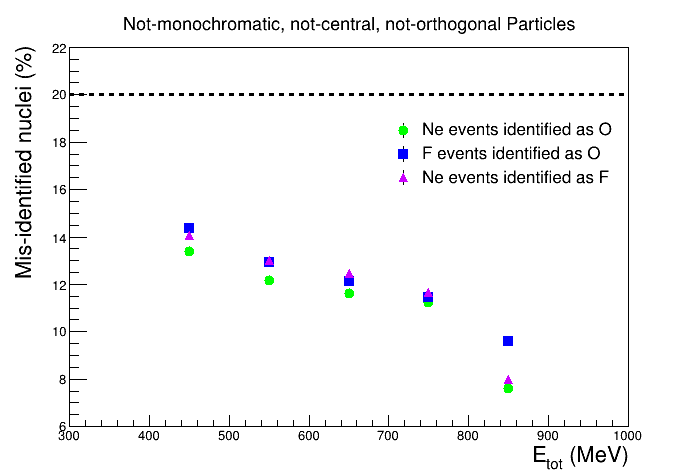
\includegraphics[scale=0.43]{Grafici_Tesi/Particelle_non_monocromatiche/leakage_alto_corr.png}}
%	\hspace{10mm}
%	\subfigure[]
%	{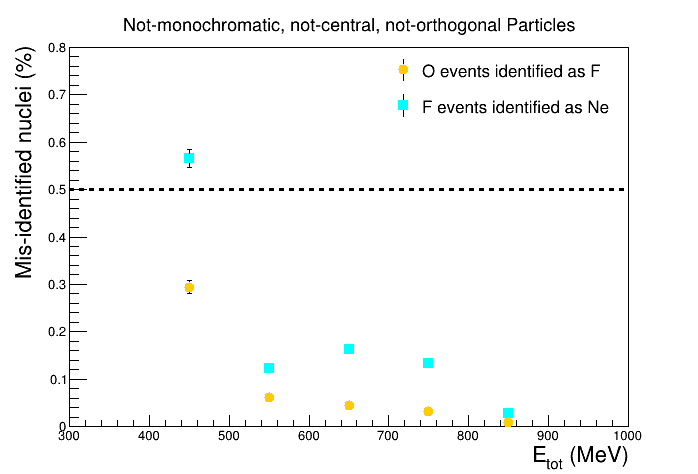
\includegraphics[scale=0.43]{Grafici_Tesi/Particelle_non_monocromatiche/leakage_basso_corr.png}}
%	\caption{La percentuale di nuclei identificati in modo erroneo in funzione di $E_{tot}$: in (a) la contaminazione da specie atomiche con $Z$ maggiore verso quelle con $Z$ minore, in (b) il viceversa. La linea tratteggiata in (a) indica il limite massimo imposto sul mancato riconoscimento del segnale, mentre in (b) rappresenta il limite massimo fissato sulla contaminazione del segnale. Laddove non sono mostrate, le barre di errore sono più piccole del marker.} \label{fig:leakage}
%\end{figure}


%%Il risultato di tale procedura è illustrato in Figura~\ref{fig:leakage}, dove il range energetico è stato suddiviso in intervalli da 100~MeV e si è scelto di rappresentare i dati soltanto laddove fossero presenti tutte e tre le bande.
%%Si può notare che la contaminazione da una specie atomica con $Z$ più grande verso una con $Z$ più piccolo è nettamente maggiore; infatti, le percentuali che si trovano in Figura~\ref{fig:leakage}.a sono comprese fra il 7\% e il 15\%, mentre quelle in Figura~\ref{fig:leakage}.b sono inferiori all'1\%.
%%In entrambi i casi si può osservare che la frazione di nuclei erroneamente identificati ha un andamento decrescente al crescere dell'energia.
%%Di conseguenza, a basse energie, dove gli effetti di raccolta parziale della carica sono maggiormente significativi, la capacità di separare gli ioni peggiora.
%%Infine, si può osservare che con la statistica simulata non si osserva una contaminazione di O in Ne, per cui si può mettere un limite superiore.







%%I due grafici in Figura~\ref{fig:leakage} sono estremamente importanti nella valutazione dell'idoneità di questo sistema di rivelazione agli scopi di NUMEN, in quanto per riuscire a misurare processi rari come quelli di DCE è essenziale che il segnale venga riconosciuto e che il fondo non venga identificato come segnale: se, ad esempio, consideriamo che il segnale da ricercare sia \ce{^{18}Ne}, allora gli eventi di tale ione identificati come \ce{^{18}O} o \ce{^{18}F} costituiscono una perdita di segnali corretti. 
%%Dunque, è necessario stabilire un limite inferiore alla probabilità di riconoscimento del segnale.
%%Ai fini di questo lavoro di tesi, tale limite può essere posto all'80\%.
%%D'altra parte, sempre considerando che il segnale sia costituito da \ce{^{18}Ne}, gli eventi di \ce{^{18}O} e \ce{^{18}F} identificati come \ce{^{18}Ne} rappresentano, invece, una contaminazione, ovvero fondo scambiato per segnale.
%%In questo caso bisogna fissare un limite superiore a tale contaminazione:
%%per gli scopi di questo lavoro, esso è stato posto allo 0.5\%.
%%Poiché gli eventi di fondo sono tipicamente molto più abbondanti di quelli di segnale, è necessario avere una selezione molto più stringente.
%%Questo evita che il numero di eventi di fondo erroneamente identificati come segnale sia comparabile con il numero dei reali eventi di segnale.

%(\textcolor{red}{Scrivere la parte sull'efficienza di riconoscimento del segnale})






%Uno studio interessante riguarda il confronto fra la correlazione $\Delta E_{SiC} - E_{tot}$ e quella $\Delta E_{SiC} - E_{CsI}$: in Figura~\ref{fig:deltaE_ERes}.
%%A questo punto, è interessante studiare la correlazione $\Delta E_{SiC} - E_{CsI}$: in Figura~\ref{fig:deltaE_ERes} sono riportate le matrici delle tre specie di interesse, le quali continuano ad essere ben separate per tutto il range energetico.
%%\begin{figure} [!p]
%	\centering
%	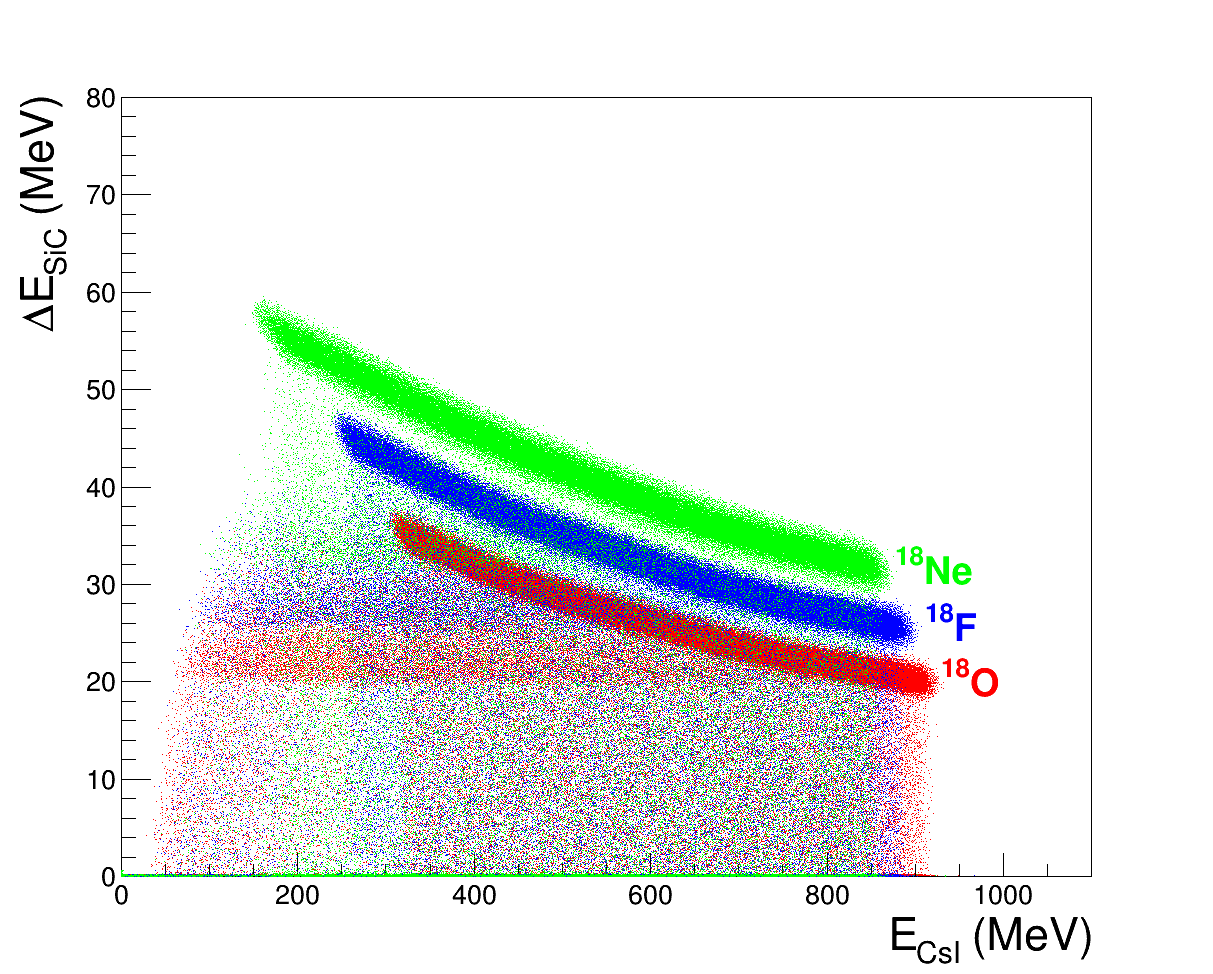
\includegraphics[width=\textwidth, keepaspectratio]{Grafici_Tesi/Particelle_non_monocromatiche_Resid/deltaE_ERes.png}
%	\caption{Matrici $\Delta E_{SiC} - E_{CsI}$.} \label{fig:deltaE_ERes}
%\end{figure} 
%Dal confronto con la Figura~\ref{fig:deltaE_ETot_full_energy} si nota che tali matrici si estendono ad energie inferiori, in quanto alla variabile sull'asse orizzontale viene a mancare il contributo di $\Delta E_{SiC}$. 
%%Confrontando tali matrici con quelle in Figura~\ref{fig:deltaE_ETot_full_energy}, non si notano sostanziali differenze, in particolare per quanto riguarda la densità degli eventi spuri.
%%Questa affermazione è supportata dalla Figura~\ref{fig:leakage_res}, nella quale si riscontrano percentuali simili a quelle viste in Figura~\ref{fig:leakage}.
%\begin{figure}[!p] 
%	\centering
%	\subfigure[]
%	{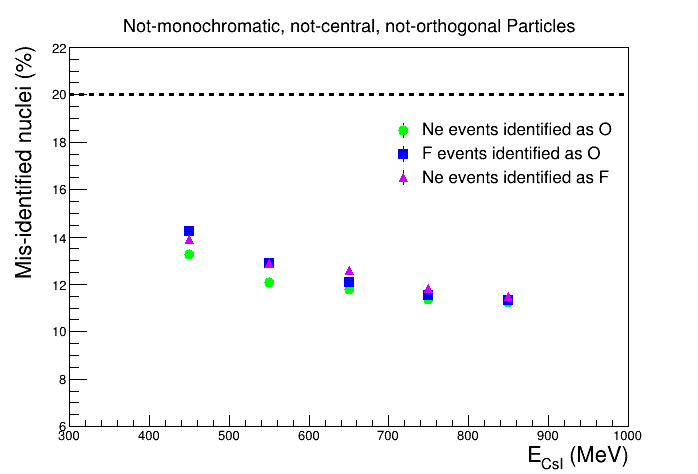
\includegraphics[scale=0.43]{Grafici_Tesi/Particelle_non_monocromatiche_Resid/leakage_alto_corr.png}}
%	\hspace{10mm}
%	\subfigure[]
%	{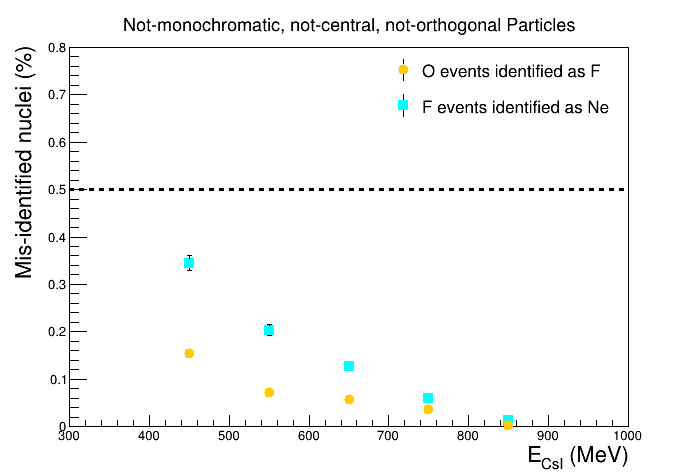
\includegraphics[scale=0.43]{Grafici_Tesi/Particelle_non_monocromatiche_Resid/leakage_basso_corr.png}}
%	\caption{La percentuale di nuclei identificati in modo erroneo in funzione di $E_{CsI}$: in (a) la contaminazione da specie atomiche con $Z$ maggiore verso quelle con $Z$ minore, in (b) il viceversa. La linea tratteggiata in (a) indica il limite massimo imposto sul mancato riconoscimento del segnale, mentre in (b) rappresenta il limite massimo fissato sulla contaminazione del segnale. Laddove non sono mostrate, le barre di errore sono più piccole del marker.} \label{fig:leakage_res}
%\end{figure}
%%L'unica differenza sembra essere dovuta al punto in Figura~\ref{fig:leakage_res}.a ad 850~MeV, per il quale si osservano percentuali lievemente maggiori del suo corrispettivo in Figura~\ref{fig:leakage}.a. 
%Ciò sembra essere legato al modo in cui si dispongono gli eventi con raccolta di carica incompleta; 
%%Ciò è legato alla correlazione delle due grandezze;
%%infatti, mentre nelle matrici $\Delta E_{SiC} - E_{tot}$ tali eventi scendono verso l'asse orizzontale con una certa inclinazione, nelle matrici $\Delta E_{SiC} - E_{CsI}$ la loro discesa verso all'asse $E_{CsI}$ procede in direzione perpendicolare. 
%%Sulla base di questo risultato è possibile sostenere che non è necessario effettuare una calibrazione energetica dei telescopi, in quanto ai fini della PID non vi è l'esigenza di sommare i valori di energia misurati dai due rivelatori.
%%Dal momento che il muro di telescopi sarà composto da oltre 1000 dispositivi, la possibilità di evitarne la calibrazione consentirebbe un notevole risparmio di tempo.
%Poiché la correlazione $\Delta E_{SiC} - E_{CsI}$ offre risultati paragonabili a quelli della correlazione $\Delta E_{SiC} - E_{tot}$, da questo momento in poi verranno presentate le matrici soltanto 











%%Poiché anche in altri casi si è riscontrato che la correlazione $\Delta E_{SiC} - E_{CsI}$ offre risultati paragonabili a quelli di $\Delta E_{SiC} - E_{tot}$, da questo momento in poi verranno presentate soltanto le matrici $\Delta E_{SiC} - E_{CsI}$.








%\vspace{0.5cm}
%\clearpage

\subsection{\iflanguage{italian}{Modello di interazioni adroniche}{Model with adronic interactions}} \label{par:interazioni_adroniche}

\begin{figure} [!p]
	\centering
	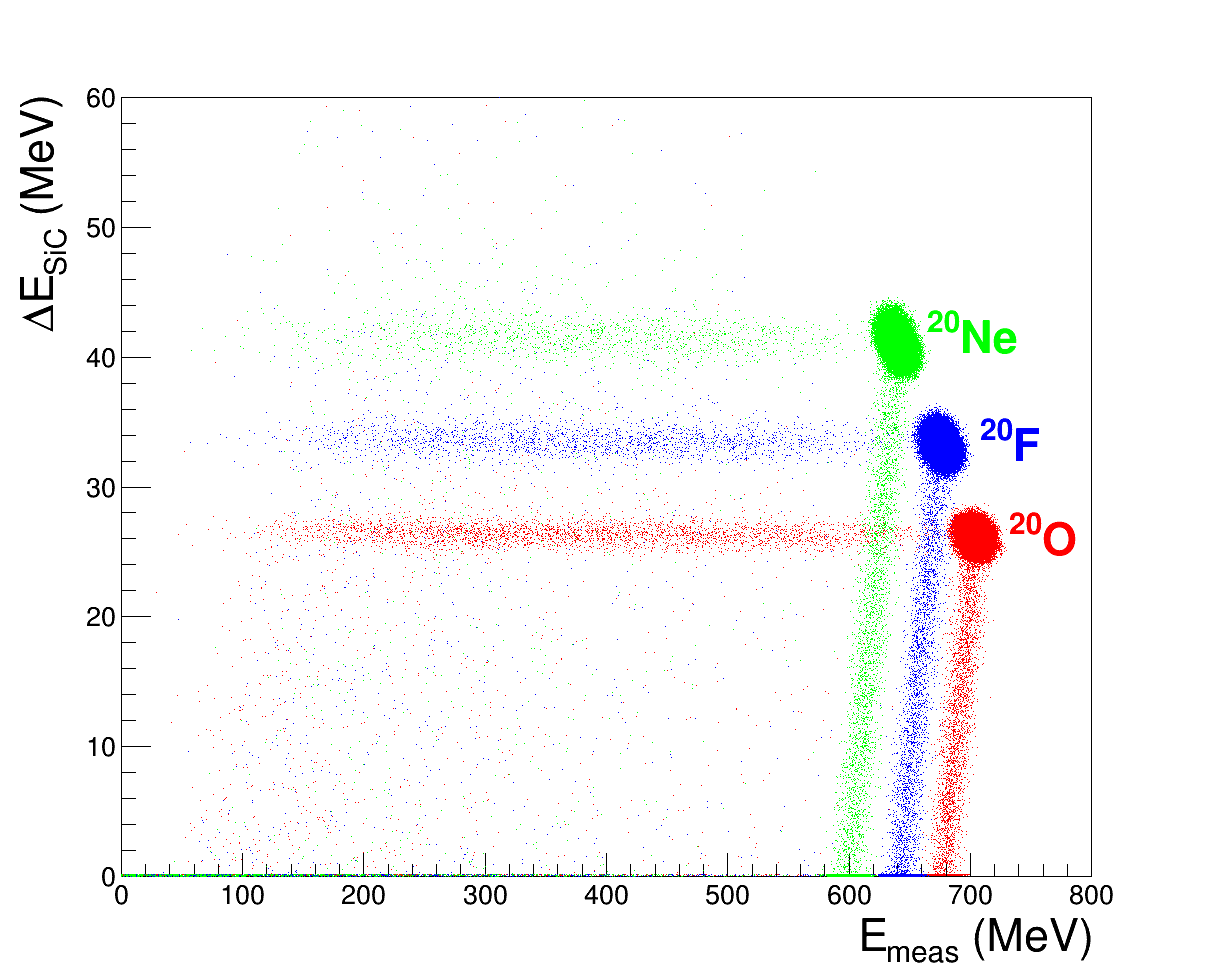
\includegraphics[width=\textwidth, keepaspectratio]{Grafici_Tesi2/Interazioni_adroniche/deltaE_ETot_quadrata.png}
	\caption{Le matrici $\Delta E_{SiC} - E_{meas}$ considerando un modello di processi fisici che comprenda anche le interazioni adroniche.} \label{fig:deltaE_ERes_adron}
\end{figure}





Rispetto all'esempio precedente, in questa simulazione la geometria e le caratteristiche delle particelle primarie restano invariate, mentre il modello dei processi fisici adesso include le interazioni adroniche. 
Le corrispondenti matrici $\Delta E_{SiC} - E_{meas}$ sono riportate in Figura~\ref{fig:deltaE_ERes_adron}: a differenza del caso in cui erano considerate soltanto le interazioni elettromagnetiche, si può osservare per tutte e tre le specie nucleari la comparsa di eventi ad un'energia $\Delta E_{SiC}$ più alta di quella dei rispettivi luoghi.
Ciò è dovuto a reazioni nucleari esotermiche, nelle quali viene rilasciata una quantità di energia aggiuntiva rispetto alla sola energia cinetica del proiettile.
%La presenza di questi eventi non sembra provocare significativi cambiamenti nelle capacità di PID, in quanto, come si può evincere dalla Figura~\ref{fig:leakage_res_adron}, le percentuali di nuclei potenzialmente male identificati aumentano di meno dell'1\%.
%L'unico mutamento degno di nota riguarda la comparsa di contaminazioni di O in Ne.
%Dunque, è evidente che la maggior parte degli eventi spuri è originata da raccolta di carica incompleta, come d'altronde era lecito aspettarsi vista la minore probabilità che avvenga un'interazione adronica.






%\begin{figure}[!p] 
%	\centering
%	\subfigure[]
%	{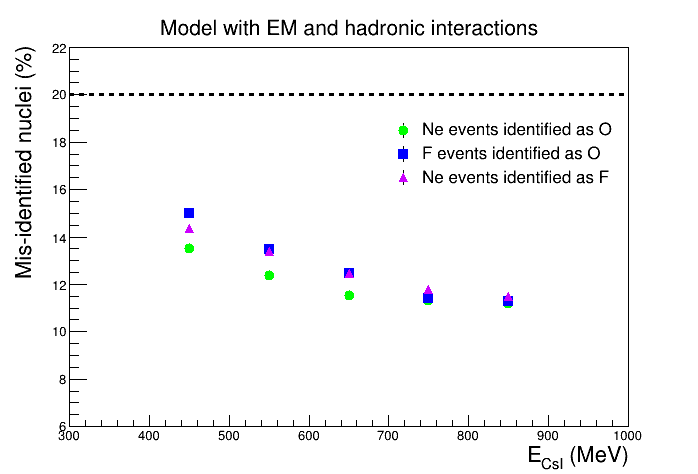
\includegraphics[scale=0.43]{Grafici_Tesi/Interazioni_adroniche/leakage_alto_corr.png}}
%	\hspace{10mm}
%	\subfigure[]
%	{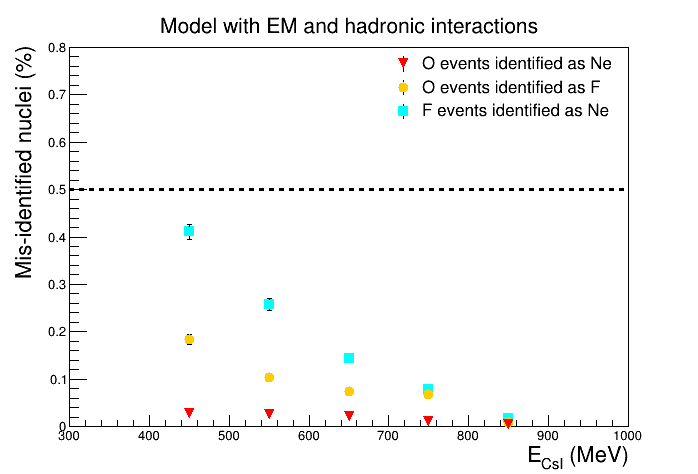
\includegraphics[scale=0.43]{Grafici_Tesi/Interazioni_adroniche/leakage_basso_corr.png}}
%	\caption{La percentuale di nuclei identificati in modo erroneo in funzione di $E_{CsI}$, utilizzando un modello che comprenda anche le interazioni adroniche: in~(a) la contaminazione da specie atomiche con $Z$ maggiore verso quelle con $Z$ minore, in (b) il viceversa. La linea tratteggiata in (a) indica il limite massimo imposto sul mancato riconoscimento del segnale, mentre in (b) rappresenta il limite massimo fissato sulla contaminazione del segnale. Laddove non sono mostrate, le barre di errore sono più piccole del marker.} \label{fig:leakage_res_adron}
%\end{figure}


%\clearpage

\subsection{\iflanguage{italian}{Studio delle capacità di PID}{Study of PID performance}}

%Uno degli obiettivi fondamentali di questo lavoro di tesi consiste nel valutare la risposta del telescopio SiC-CsI agli eventi  

Dopo aver esposto tre casi ideali, utili per comprendere alcuni fenomeni rilevanti incontrati in questo studio, si esamina adesso una situazione realistica, in cui alla simulazione \geant{} viene dato in input il file prodotto dai software per il trasporto degli eiettili.
In questo caso, dunque, gli ioni presentano sia le correlazioni cinematiche sia quelle legate allo spettrometro.
A differenza dei casi precedenti, si sono simulati nove ioni, tutti completamente ionizzati, ossia \ce{^{18}O^{8+}}, \ce{^{19}O^{8+}}, \ce{^{20}O^{8+}}, \ce{^{18}F^{9+}}, \ce{^{19}F^{9+}}, \ce{^{20}F^{9+}}, \ce{^{18}Ne^{10+}}, \ce{^{19}Ne^{10+}} e \ce{^{20}Ne^{10+}}.
Il telescopio ha dimensioni trasversali di 1.5~cm $\times$ 1.5~cm ed è posto a 14~cm di distanza dal piano in cui vengono prodotte le particelle primarie, che coincide con il piano di ingresso nel FDP.

Per fissare la rigidità magnetica di riferimento si è scelto il \ce{^{18}Ne^{10+}}, che fra gli ioni considerati è quello con il rapporto massa su carica più piccolo.
In questo modo, dovendo mantenere costante il prodotto $\sqrt{m}/q \cdot \sqrt{E}$, gli altri ioni hanno energia cinetica inferiore.
Questa considerazione è confermata dalla Figura~\ref{fig:KinE}.a, in cui viene illustrato lo spettro delle energie cinetiche dei diversi ioni.
\begin{figure} [!p]
	\centering
	\subfigure[]
	{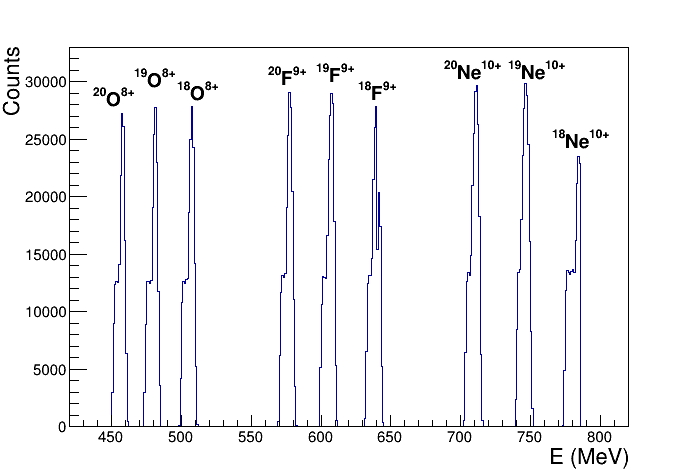
\includegraphics[scale=0.479]{Grafici_Tesi2/PID/KinE2.png}}
	%\vspace{7mm}
	\subfigure[]
	{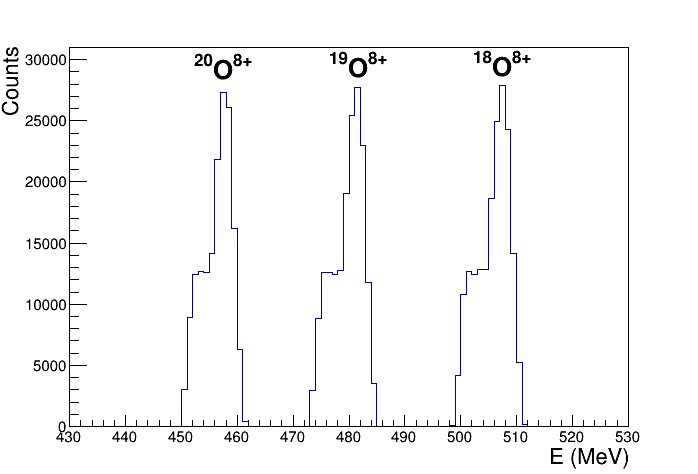
\includegraphics[scale=0.479]{Grafici_Tesi2/PID/KinE_zoom.png}}
	
	\caption{Lo spettro delle energie cinetiche~$E$ degli ioni simulati: in (a) per tutte le specie, in (b) per i soli ioni di ossigeno.} \label{fig:KinE}
\end{figure}
Da tale figura si evince che le energie cinetiche accettate dal telescopio sono molto differenti per i diversi ioni, con una differenza fra lo ione più energetico e quello meno energetico di oltre 350~MeV.
La Figura~\ref{fig:KinE}.b mostra un ingrandimento della precedente nella zona degli ioni di ossigeno: come si può notare, per ogni ione il range energetico che arriva sul telescopio è di circa 8~MeV, in buon accordo con la~\ref{eq:finestra_Brho}.
%Gli ioni hanno la stessa finestra di rigidità magnetica, per cui tutti vanno a finire sul telescopio simulato. 


%\begin{figure} [!p]
%	\centering
%	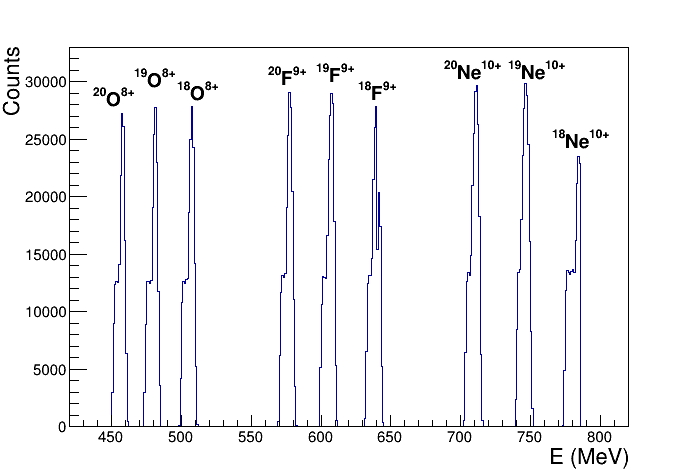
\includegraphics[scale=0.4]{Grafici_Tesi2/PID/KinE2.png}
%	\caption{Lo spettro delle energie cinetiche~$E$ dei diversi ioni simulati.} \label{fig:KinE}
%\end{figure}

%\begin{figure} [!p]
%	\centering
%	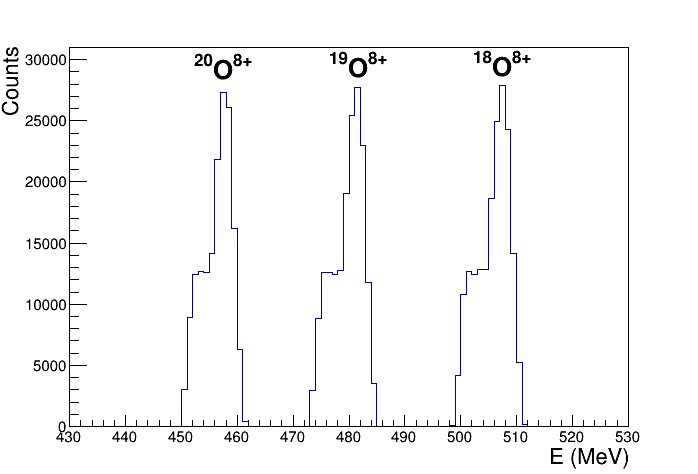
\includegraphics[scale=0.4]{Grafici_Tesi2/PID/KinE_zoom.png}
%	\caption{Ingrandimento della spettro in Figura~\ref{fig:KinE} nella zone degli ioni di ossigeno.} \label{fig:KinE_zoom}
%\end{figure}


\begin{figure} [!p]
	\centering
	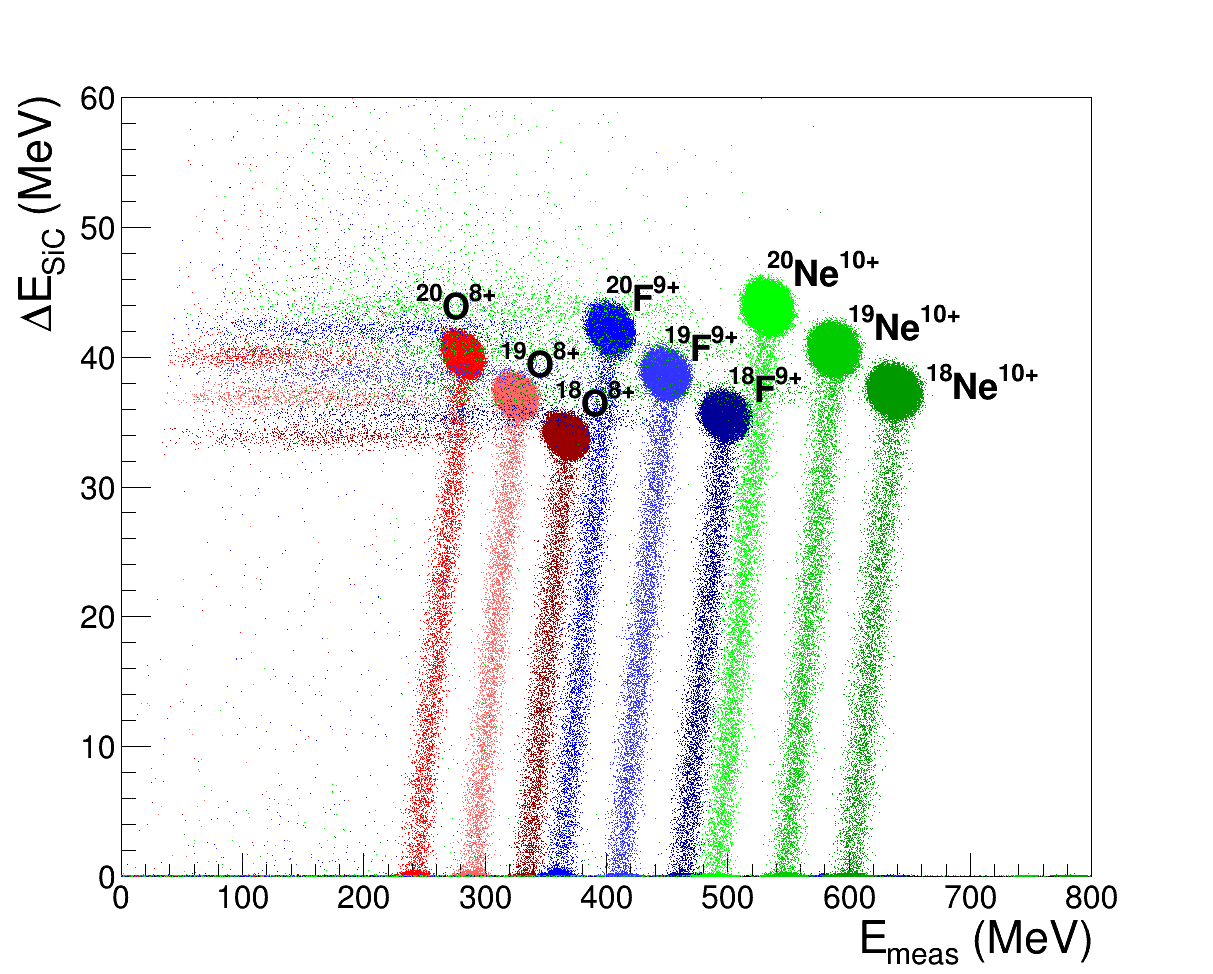
\includegraphics[width=\textwidth, keepaspectratio]{Grafici_Tesi2/PID/deltaE_Emeas_quadrata3.png}
	\caption{Le matrici $\Delta E_{SiC} - E_{meas}$ considerando per tutti gli ioni sia la cinematica di reazione sia il trasporto ottico.} \label{fig:deltaE_Emeas_PID}
\end{figure}


Le corrispondenti matrici $\Delta E_{SiC} - E_{meas}$ sono riportate in Figura~\ref{fig:deltaE_Emeas_PID}: come si può notare, i luoghi degli ioni simulati appaiono ben separati sia in numero atomico~($Z$) sia in numero di massa~($A$).
Si può, inoltre, osservare che l'energia rilasciata nel rivelatore al~SiC è molto simile per le tre specie atomiche: 
%ciò dipende dalla notevole differenza in energia cinetica degli ioni che compensa la variazione legata al cambiamento di $Z$.
ciò dipende dal fatto che, a causa del filtro in $B \rho$, gli ioni con carica $q$ più piccola hanno energia cinetica minore, mentre quelli con $q$ più grande hanno energia cinetica maggiore; ricordando che nella formula di Bethe-Bloch la perdita di energia è proporzionale a $Z^2$ e inversamente proporzionale ad $E$, si può dedurre che la notevole differenza in energia cinetica degli ioni compensa la variazione legata al cambiamento di $Z$.
%Di conseguenza, assumendo di essere interessati ad una reazione di DCE in cui si vuole rivelare l'\ce{^{20}O}, la principale componente di contaminazione nell'identificazione proviene dagli ioni che non si fermano nel rivelatore al~CsI.
Di conseguenza, nel caso in esame la principale componente di contaminazione nell'identificazione degli eventi di interesse proviene dagli ioni che non si fermano nel rivelatore al~CsI.
%Di conseguenza, nel caso in esame la principale componente di contaminazione nella PID proviene dagli ioni che non si fermano nel rivelatore al~CsI.
Per dare una stima quantitativa della percentuale di eventi degradati che potrebbero costituire un fondo nella regione di interesse (Region Of Interest, ROI), si è proceduto nel modo seguente: supponendo di voler analizzare una reazione di DCE in cui si vuole rivelare l'\ce{^{20}O}, si è effettuato nel plot $\Delta E_{SiC} - E_{meas}$ un taglio grafico attorno al luogo pertinente a tale ione, come mostrato in Figura~\ref{fig:deltaE_Emeas_taglio}.
\begin{figure} [!p]
	\centering
	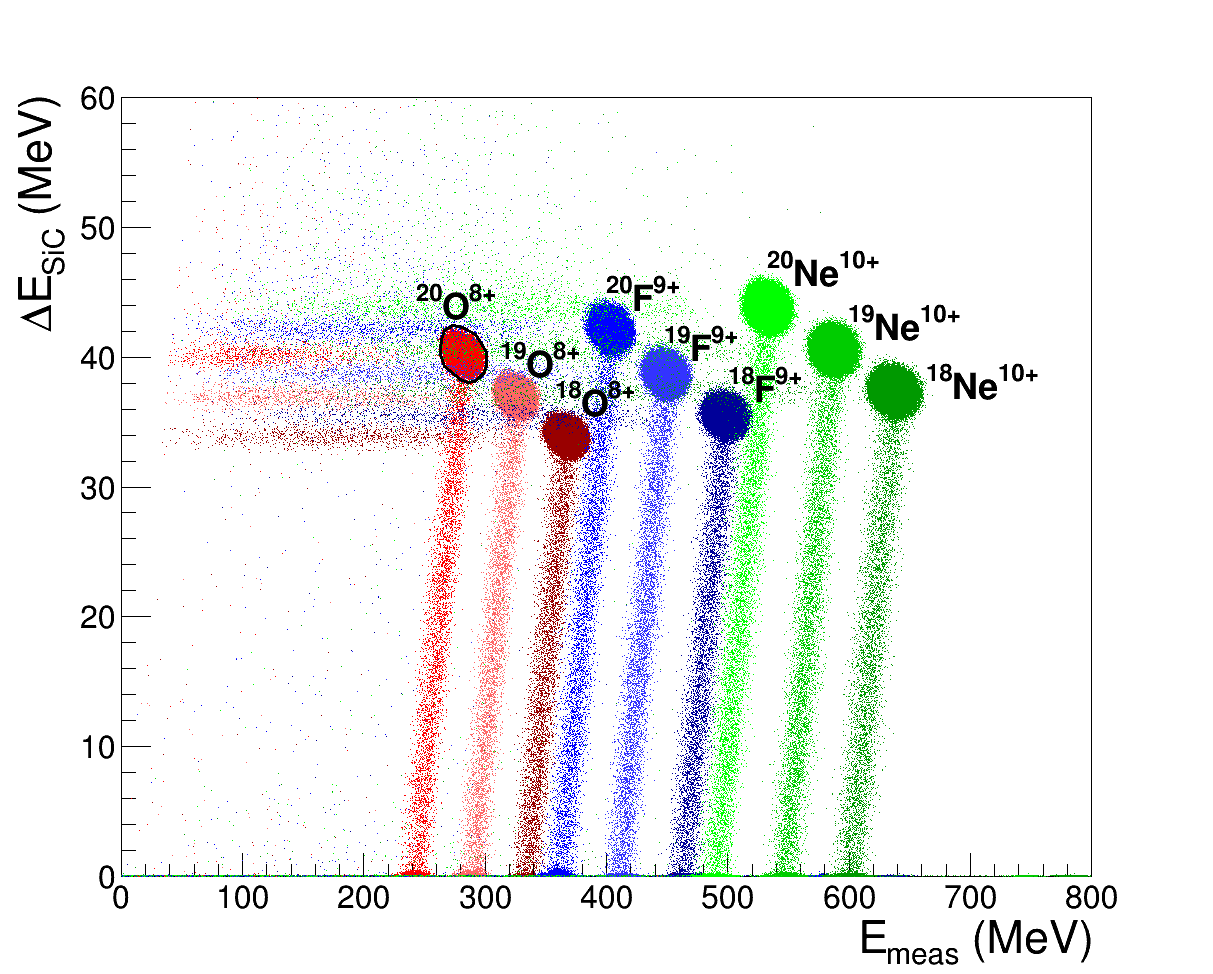
\includegraphics[width=\textwidth, keepaspectratio]{Grafici_Tesi2/PID/deltaE_Emeas_quadrata_taglio_label.png}
	\caption{Taglio grafico per l'identificazione dell'\ce{^{20}O^{8+}} e per il calcolo delle percentuali di contaminazione.} \label{fig:deltaE_Emeas_taglio}
\end{figure}
All'interno del taglio sono presenti, oltre allo ione di interesse, anche altre specie ioniche, che potrebbero essere erroneamente identificate come~\ce{^{20}O^{8+}}.
La percentuale di contaminazione nella ROI dovuta ad un particolare ione può essere calcolata dividendo il numero di eventi di quello ione presenti nella ROI per il numero totale di eventi dello stesso.
%Supponiamo, adesso, di essere interessati ad una reazione di DCE in cui si vuole rivelare l'\ce{^{20}O}: il primo passo nell'analisi dei dati consiste nell'identificazione degli ioni di interesse attraverso l'utilizzo di tagli grafici.
Il risultato di tale operazione, nel caso del taglio grafico considerato in Figura~\ref{fig:deltaE_Emeas_taglio}, è riportato in Tabella~\ref{tab:contaminazione_deltaE_Emeas_1.5per1.5}: come si può notare, le percentuali sono molto basse, a dimostrazione delle grandi capacità di PID del telescopio~SiC-CsI.
\begin{table} [t!]
	\begin{center}
		\renewcommand{\arraystretch}{1.2}
		\begin{tabular} {cccc}
			Ione               & & &   Contaminazione nella ROI (\%) \\
			\toprule[0.1em]
			%\hline
			\ce{^{18}O^{8+}}   & & &   0.002 $\pm$ 0.001 \\
			\ce{^{19}O^{8+}}   & & &   0.001 $\pm$ 0.001 \\
			\ce{^{18}F^{9+}}   & & &   0.017 $\pm$ 0.003 \\
			\ce{^{19}F^{9+}}   & & &   0.100 $\pm$ 0.007 \\
			\ce{^{20}F^{9+}}   & & &   0.057 $\pm$ 0.005 \\
			\ce{^{18}Ne^{10+}} & & &   0.031 $\pm$ 0.004 \\
			\ce{^{19}Ne^{10+}} & & &   0.089 $\pm$ 0.006 \\
			\ce{^{20}Ne^{10+}} & & &   0.002 $\pm$ 0.001 \\
		\end{tabular}
	\end{center}
	\caption{La contaminazione dei diversi ioni nella ROI dell'\ce{^{20}O^{8+}} individuata dal taglio grafico in Figura~\ref{fig:deltaE_Emeas_taglio}.} \label{tab:contaminazione_deltaE_Emeas_1.5per1.5}
\end{table}
La contaminazione più rilevante deriva dal \ce{^{19}F^{9+}} e dal \ce{^{19}Ne^{10+}}, come era lecito aspettarsi considerando che si tratta delle specie ioniche che hanno un valore di $\Delta E_{SiC}$ molto simile a quello dell'\ce{^{20}O^{8+}}.
La percentuale di eventi di~\ce{^{20}O^{8+}} persi nell'identificazione può essere determinata dividendo il numero di eventi di~\ce{^{20}O^{8+}} al di fuori della ROI per il numero totale di eventi dello stesso: dal calcolo risulta che tale percentuale è del~$(9.14 \pm 0.08)$~\%.
Questa è la frazione di eventi corretti che viene persa a causa dell'incompleta raccolta di carica nel rivelatore al~SiC o del parziale rilascio dell'energia residua nel cristallo allo~CsI.



Per riprodurre più correttamente la situazione reale, bisogna tenere presente che nello spettrometro magnetico possono essere trasportati anche ioni in stati di carica diversi. 
Questi derivano da una componente di particelle non completamente ionizzata presente all'interno del fascio e da ioni che, attraversando la materia, strappano uno o più elettroni.
È stata, dunque, svolta una simulazione considerando le seguenti specie ioniche: \ce{^{20}O^{8+}}, \ce{^{18}F^{8+}}, \ce{^{19}F^{8+}}, \ce{^{20}F^{8+}}, \ce{^{18}Ne^{8+}}, \ce{^{19}Ne^{8+}} e \ce{^{20}Ne^{8+}}; tali particelle hanno, infatti, un rapporto $\sqrt{m}/q$ molto vicino a quello degli ioni precedentemente considerati, per cui possono incidere sullo stesso telescopio.
Anche in questo caso, le energie cinetiche sono state determinate in modo che gli ioni avessero lo stessa finestra di rigidità magnetica.
\begin{figure} [!p]
	\centering
	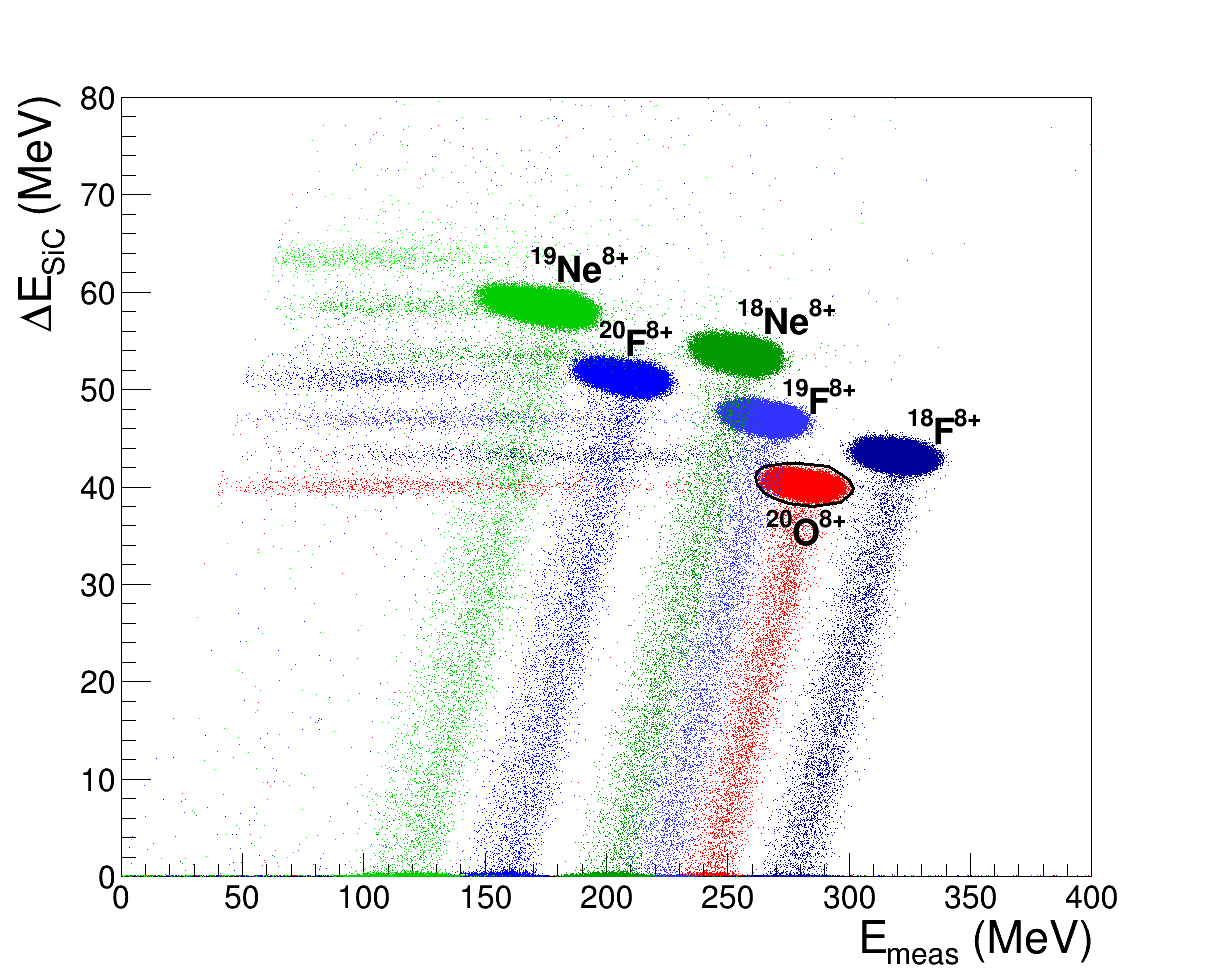
\includegraphics[width=\textwidth, keepaspectratio]{Grafici_Tesi2/PID/deltaE_Emeas_stati_carica_taglio2.png}
	\caption{Le matrici $\Delta E_{SiC} - E_{meas}$ per ioni con rapporto $\sqrt{m}/q$ simile a quello dell'\ce{^{20}O^{8+}}. Viene, inoltre, mostrato il taglio grafico per l'identificazione dell'\ce{^{20}O^{8+}} e per il calcolo delle percentuali di contaminazione.} \label{fig:deltaE_Emeas_PID_stati_carica}
\end{figure} 
Le matrici $\Delta E_{SiC} - E_{meas}$ corrispondenti sono mostrate in Figura~\ref{fig:deltaE_Emeas_PID_stati_carica}: come si può notare, anche in questa simulazione i luoghi delle specie ioniche appaiono ben distinti.
Inoltre, si fa osservare che nel plot non appare il luogo del~\ce{^{20}Ne^{8+}} poiché la sua energia cinetica non è sufficiente a fargli attraversare il substrato passivato del rivelatore al~SiC.
Supponendo di essere ancora interessati ad identificare l'\ce{^{20}O^{8+}}, la principale componente di contaminazione scaturisce in questo caso dagli eventi affetti da raccolta di carica incompleta.
Se si effettua un taglio grafico come quello riportato in figura, si può procedere alla stima delle contaminazioni in modo analogo a quello appena discusso.
%I risultati sono mostrati in Tabella~\ref{tab:contaminazione_deltaE_Emeas_1.5per1.5_stati_carica}: il maggiore contaminante risulta essere il~\ce{^{19}F^{8+}}, in quanto la sua matrice va a posizionarsi ad una~$E_{meas}$ molto simile a quella dell'\ce{^{20}O^{8+}}.
I risultati sono mostrati in Tabella~\ref{tab:contaminazione_deltaE_Emeas_1.5per1.5_stati_carica}: in questo caso soltanto il~\ce{^{18}F^{8+}} e il~\ce{^{19}F^{8+}} fanno da contaminanti per l'\ce{^{20}O^{8+}}, con il secondo che contribuisce in maniera nettamente superiore rispetto al primo.
La percentuale di eventi di \ce{^{20}O^{8+}} che si colloca al di fuori della ROI è del $(9.25 \pm 0.08)$~\%, compatibile con il valore precedentemente stimato.


\begin{table} [t!]
	\begin{center}
		\renewcommand{\arraystretch}{1.2}
		\begin{tabular} {cccc}
			Ione               & & &   Contaminazione nella ROI (\%) \\
			\toprule[0.1em]
			%\hline
			%	\ce{^{19}O^{8+}}   & & &   0.001 $\pm$ 0.001 \\
			\ce{^{18}F^{8+}}   & & &   0.002 $\pm$ 0.001 \\
			\ce{^{19}F^{8+}}   & & &   0.051 $\pm$ 0.005 \\
		\end{tabular}
	\end{center}
	\caption{La contaminazione di ioni con rapporto $\sqrt{m}/q$ simile a quello dell'\ce{^{20}O^{8+}} nella ROI individuata dal taglio grafico in Figura~\ref{fig:deltaE_Emeas_PID_stati_carica}.} \label{tab:contaminazione_deltaE_Emeas_1.5per1.5_stati_carica}
\end{table}

A questo punto è bene sottolineare che le percentuali riportate sono state calcolate simulando per tutti gli ioni lo stesso numero di eventi.
Tuttavia, nella situazione reale la produzione degli ioni considerati avviene attraverso meccanismi di reazioni nucleari, ciascuno caratterizzato da una certa sezione d'urto; questa rappresenta, infatti, la probabilità con cui può verificarsi una determinata reazione.  
I valori tipici delle sezioni d'urto sperimentali dei processi coinvolti in questa simulazione, normalizzati alla sezione d'urto sperimentale peculiare del DCE, sono riportati nella Tabella~\ref{tab:sez_d'urto}, insieme alla probabilità di avere uno ione in un certo stato di carica dopo il passaggio attraverso un foglio di carbonio.
Moltiplicando il valore della sezione d'urto sperimentale tipica di un processo per la probabilità di ottenere uno stato di carica, si può determinare la probabilità di produrre, a seguito di una reazione nucleare, uno ione in un determinato stato di carica;
%%Moltiplicando i numeri della terza colonna con quelli della quarta, si può determinare la probabilità di ottenere, a seguito di una reazione nucleare, uno ione in un determinato stato di carica.
questo è il fattore con cui bisogna riscalare le percentuali precedentemente mostrate per stimare le contaminazioni reali.
Il risultato di questa operazione è riportato in Tabella~\ref{tab:contaminazioni_riscalate}



%\begin{table} [t!]
%	\begin{center}
%		\renewcommand{\arraystretch}{1.2}
%		\begin{tabular} {ccccccc}
%			Reazione & & Ione & & \multirow{2}{35 mm}{Sez. d'urto sperim. norm. al DCE}  & & Fraz. di stato di carica \\
%			         & &      & &        & &                          \\
%			\toprule
%			%\hline
%			DCE  & & \ce{^{20}O} & &  1  & & $8+ \rightarrow 0.9987$ \\
%			\hline
%			DCE  & & \ce{^{20}O} & &  1  & & $8+ \rightarrow 0.9987$ \\
%		\end{tabular}
%	\end{center}
%\end{table}
%\clearpage
\begin{table} [p!]
	\begin{center}
		\renewcommand{\arraystretch}{1.2}
		\begin{tabular} {cccccccl}
			Reazione & & Ione & & Sez. d'urto sperim.  & & \multicolumn{2}{c}{Fraz. di stato di carica}  \\
			         & &      & &    norm. al DCE    & &&                          \\
			\toprule[0.1em]
			%\hline
			DCE        & & \ce{^{20}O}  & &        1        & & & $8^+ \sim 0.9987$ \\
			\hline
			SCE        & & \ce{^{20}F}  & &     $10^4$      & & & $9^+ \sim 0.99934$ \\
			           & &              & &                 & & & $8^+ \sim 10^{-4}$ \\
   			\hline
			1-proton   & & \ce{^{19}F}  & &  $2\cdot10^4 $  & & & $9^+ > 0.99934$ \\
                       & &              & &                 & & & $8^+ < 10^{-4}$ \\
			\hline
			1-neutron  & & \ce{^{19}Ne} & &  $3\cdot10^4 $  & & & $10^+ > 0.99905$ \\
                       & &              & &                 & & & $9^+ < 10^{-5}$ \\
                       & &              & &                 & & & $8^+ < 10^{-7}$ \\
   			\hline
			2-proton   & & \ce{^{18}O}  & &     $10^3$      & & & $8^+ > 0.99963$ \\
			\hline
			2-neutron  & & \ce{^{18}Ne} & &     $10^2 $     & & & $10^+ > 0.99905$ \\
                       & &              & &                 & & & $9^+ < 10^{-5}$ \\
                       & &              & &                 & & & $8^+ < 10^{-7}$ \\
			\hline
			1-deuteron & & \ce{^{18}F}  & &     $10^3 $     & & & $9^+ > 0.99934$ \\
                       & &              & &                 & & & $8^+ < 10^{-4}$ \\
            \hline
            2-p 1-n    & & \ce{^{19}O}  & &        10       & & & $8^+ \sim 0.99963$ \\
            \hline
            inelastic  & & \ce{^{20}Ne} & &     $10^4 $     & & & $10^+ > 0.99905$ \\
                       & &              & &                 & & & $9^+ < 10^{-5}$ \\
                       & &              & &                 & & & $8^+ < 10^{-7}$ \\
            \bottomrule[0.1em]
		\end{tabular}
	\end{center}
	\caption{I valori tipici delle sezioni d'urto sperimentali di diversi processi di reazioni nucleari normalizzate alla sezione d'urto del DCE. Si riporta, inoltre, la probabilità di avere uno ione in un determinato stato di carica dopo aver attraversato un foglio di carbonio.} \label{tab:sez_d'urto}
\end{table}


%\begin{table} [h!]
%	\begin{center}
%		\renewcommand{\arraystretch}{1.2}
%		\begin{tabular} {ccccccrcl}
%			Reazione & & Ione & & Sez. d'urto sperim.  & & \multicolumn{3}{c}{Fraz. di stato di carica} \\
%			& &      & &    norm. al DCE    & &   & &          \\
%			\toprule
%			%\hline
%			DCE       & & \ce{^{20}O} & &        1        & & $8^+$ & $\rightarrow$ & 0.9987 \\
%			\hline
%			SCE       & & \ce{^{20}F} & &     $10^4$      & & $9^+$ & $\rightarrow$ &0.99934 \\
%			& &             & &                 & & $8^+$ & $\rightarrow$ & $10^{-4}$ \\
%			\hline
%			1-proton  & & \ce{^{19}F} & &  $2\cdot10^4 $  & & $9^+$ &      >        & 0.99934 \\
%			& &             & &                 & & $8^+$ &      <        & $10^{-4}$ \\
			
%		\end{tabular}
%	\end{center}
%\end{table}



%\begin{table}[t!]
%	\begin{center}
%		\begin{tabular}{ccc}
%			Nuclide       & &  Energia [MeV] \\
%			\toprule
%			\ce{^{16}O}  &  &  724.3 \\
%			\ce{^{17}O}  &  &  683.3 \\
%			\ce{^{18}O}  &  &  646.8 \\
%			\ce{^{19}F}   & &  773.6 \\
%			\ce{^{20}F}   & &  736.4 \\
%			\ce{^{18}Ne}  & &  1000  \\
%			\ce{^{19}Ne}  & &  950.3 \\
%			\ce{^{20}Ne}  & &  905.4
%		\end{tabular}
%	\end{center}
%	\caption{I valori di energia corrispondenti ad una rigidità magnetica di 1.96~T$\cdot$m per i diversi nuclidi.
%		\label{tab:energia}}
%\end{table}


\begin{table} [p!]
	\begin{center}
		\renewcommand{\arraystretch}{1.2}
		\begin{tabular} {cccccc}
			Ione &  Stato di carica & & Numero di eventi nella ROI  & &  Contaminazione\\
			     &                  & &   norm. ad 1 evento di DCE  & &  
			nella ROI (\%)\\
			\toprule[0.1em]
			%\hline
			\ce{^{18}O}    &  $8^+$   & &  $0.017 \pm 0.010$      & & $0.0309 \pm 0.0002$\\
			\hline
			\ce{^{19}O}    &  $8^+$   & &  $0.00006 \pm 0.00006$  & & $ \sim 10^{-4}$\\
			\hline
			\ce{^{20}O}    &  $8^+$   & &  $0.907 \pm 0.002$      & & $1.6934 \pm 0.0008$\\
			\hline
			\ce{^{18}F}    &  $9^+$   & &  $0.17 \pm 0.03$        & & $0.3159 \pm 0.0006$\\
						   &  $8^+$   & &  $ \sim 10^{-6}$        & & $\sim 10^{-6}$\\
			\hline
			\ce{^{19}F}    &  $9^+$   & &  $20 \pm 1$             & &\\
						   &  $8^+$   & &  $ 0.010 \pm 0.0001$    & &\\
			\hline
			\ce{^{20}F}    &  $9^+$   & &  $5.7 \pm 0.5$          & &\\
			\hline
			\ce{^{18}Ne}   &  $10^+$  & &  $0.031 \pm 0.004$      & &\\
			\hline
			\ce{^{19}Ne}   &  $10^+$  & &  $27 \pm 2$             & &\\
			\hline
			\ce{^{20}Ne}   &  $10^+$  & &  $0.14 \pm 0.08$        & &\\
			\bottomrule[0.1em]
		\end{tabular}
	\end{center}
	\caption{I valori tipici delle sezioni d'urto sperimentali di diversi processi di reazioni nucleari normalizzate alla sezione d'urto del DCE. Si riporta, inoltre, la probabilità di avere uno ione in un determinato stato di carica dopo aver attraversato un foglio di carbonio.} \label{tab:contaminazioni_riscalate}
\end{table}



%A questo punto è interessante mostrare le correlazioni $x_{foc} - E$


%L'integrazione fra i software dedicati al trasporto ottico degli eiettili e la simulazione del telescopio permette di ricavare altre importanti correlazioni, utili per la PID.
%In Figura~ sono mostrate le matrici $x_{foc} - E_{meas}$ relative al caso in esame:



Da continuare...


\chapter{\iflanguage{italian}{Validazione della simulazione \geant}{Validation of \geant simulation}}

All'interno dell'intensa campagna di studi condotta per verificare se le soluzioni previste per il progetto NUMEN possano garantire le prestazioni richieste, è stato svolto ad Aprile 2019 un test beam sui primi due prototipi di telescopi basati sulla tecnologia SiC-CsI.
Tale test si è tenuto ai Laboratori Nazionali del Sud (LNS) utilizzando un fascio di particelle di \ce{^{20}Ne} a 20~AMeV, prodotto dal Ciclotrone Superconduttore K800.
Al fine di favorire la generazione degli ioni di interesse per NUMEN, ovvero Ossigeno, Fluoro e Neon, si è scelto di utilizzare un bersaglio di \ce{^{12}C} da 400~$\mu$g/cm\ap{2}.

Il test aveva l'obiettivo di valutare la risposta dei telescopi e di confrontare l'elettronica tradizionale di MAGNEX con la nuova elettronica VMM3a~\cite{degeronimo:ieee13} per il progetto.
%In questo capitolo vengono presentati i dati sperimentali ottenuti durante tale test e viene mostrato il confronto tra questi e i risultati del tool di simulazioni implementato per questo lavoro di tesi.
%Tale confronto ha lo scopo di validare il tool
In questo capitolo vengono presentati i dati sperimentali ottenuti durante tale test e, attraverso il confronto tra questi e i dati simulati, viene validato il tool di simulazioni sviluppato per questo lavoro di tesi.
Dal momento che i prototipi utilizzati nel test presentano alcune differenze rispetto ai telescopi che verranno impiegati per NUMEN, è stato necessario modificare alcuni parametri della simulazione: in primo luogo, ricordando che, in uno dei due dispositivi (Tel~A), il primo stadio era montato in configurazione reverse, il substrato epitassiale del rivelatore al SiC è stato posto davanti al volume sensibile.
Inoltre, le dimensioni trasversali e gli spessori delle diverse componenti sono state cambiate in modo da riprodurre le caratteristiche descritte nel Paragrafo~\ref{par:telescopi}.


\section{\iflanguage{italian}{I dati del telescopio SiC-CsI}{Data of SiC-CsI telescope}}


Gli eiettili prodotti nell'interazione fra proiettile e bersaglio, dopo aver attraversato il quadrupolo e il dipolo, giungono al rivelatore di piano focale (Focal Plane Detector, FPD) di MAGNEX, dove, in occasione del test, erano stati posti i due telescopi, chiamati Tel~A e Tel~B. 
Come descritto nella Sezione~\ref{sez:test}, insieme ai due telescopi, erano stati montati quattro dei rivelatori al silicio attualmente in uso, i quali servivano da riferimento e da confronto per la Particle IDentification (PID).

Poiché all'energia utilizzata nel test i prodotti di reazione non erano in grado di superare il substrato epitassiale del Tel~B, da tale telescopio era possibile estrarre soltanto il segnale sulla perdita di energia, non permettendo di riprodurre le correlazioni $\Delta E - E_{resid}$ utili per l'identificazione in numero atomico $Z$ degli ioni.
Di conseguenza, dal momento che questo lavoro aveva lo scopo di studiare le performance di PID di tale sistema, sono stati analizzati soltanto i dati relativi al Tel~A.


%\subsection{\iflanguage{italian}{Le matrici $\Delta E_{SiC} - E_{CsI}$}{$\Delta E_{SiC} - E_{CsI}$ matrices}}
%Indicando con $\Delta E_{SiC}$ la perdita di energia misurata dal rivelatore al~SiC e con $E_{CsI}$ l'energia misurata dallo scintillatore allo~CsI

Indicando con $\Delta E_{SiC}$ ed $E_{CsI}$ la perdita di energia e l'energia residua, misurate, rispettivamente, dal rivelatore al~SiC e dallo scintillatore allo~CsI, in Figura~\ref{fig:sic_csi_standard} è riportata la matrice $\Delta E_{SiC} - E_{CsI}$ registrata dal Tel~A utilizzando l'elettronica standard (si veda il Paragrafo~\ref{par:elettr_standard}): come si può notare i luoghi dei diversi ioni appaiono ben separati in una regione che va dal Boro (B) al Neon (Ne).
Si può, inoltre, osservare che, poiché ai fini della PID non è necessario utilizzare la correlazione $\Delta E_{SiC} - E_{meas}$, laddove $E_{meas} = \Delta E_{SiC} + E_{CsI}$, i rivelatori non sono stati calibrati e, conseguentemente, le variabili $\Delta E_{SiC}$ e $E_{CsI}$ sono misurate in canali.


\begin{figure} [!p]
	\centering
	\includegraphics[width=\textwidth, keepaspectratio]{Grafici_Tesi2/Confronto/desic_ecsi.png}
	\caption{Le correlazioni $\Delta E_{SiC} - E_{CsI}$ ottenute dal Tel~A durante il test utilizzando la catena elettronica standard. La linea nera indica il taglio grafico effettuato per la selezione in numero atomico dell'Ossigeno.} \label{fig:sic_csi_standard}
\end{figure}




%Alla luce di questo risultato, il telescopio SiC-CsI sembra, dunque, rispondere alle richieste del progetto.
%Ricordando che questo telescopio era montato in configurazione reverse, si può anche osservare che il substrato epitassiale da 100~$\mu$m non sembra influire negativamente sulle sue proprietà di identificazione. 

%Ciò consente, dunque, di selezionare 

%Per confrontare le prestazioni di questo sistema con quelle solitamente ottenute utilizzando la co


%A questo punto può essere utile confrontare le prestazioni di questo sistema con quelle dell'apparato standard di MAGNEX, nel quale l'identificazione in numero atomico degli ioni avviene correlando la misura dell'energia persa $\Delta E$ nel gas con quella dell'energia residua $E_{resid}$ nei rivelatori al silicio; in particolare, la perdita di energia nel gas è data dalla somma delle sei perdite di energia $\Delta E_i$ misurate dai fili proporzionali.
%Inoltre, dal momento che la perdita di energia dipende dalla lunghezza della traiettoria dello ione all'interno del FPD, essa viene corretta, evento per evento, moltiplicando per il coseno dell'angolo di incidenza $\theta_{foc}$, ovvero 
%\begin{equation}
%	\Delta E^{corr}_{tot} \, = \, \frac{\cos \theta_{foc}}{\cos \theta_{tilt}} \, \sum_{i=1}^{6} \Delta E_i
%\end{equation}
%laddove $\theta_{tilt}$ rappresenta l'angolo di rotazione del FPD, pari a 59.2\textdegree.
In Figura~\ref{fig:sic_csi_vmm3a} si riporta la  matrice $\Delta E_{SiC} - E_{CsI}$ ottenuta con lo stesso telescopio utilizzando l'elettronica VMM3a (si veda il Paragrafo~\ref{par:elettr_vmm3a}): in questo caso si può notare che, sebbene si possano ancora riconoscere i luoghi corrispondenti ai diversi ioni, essi risultano parzialmente sovrapposti.
Ciò deriva da un maggiore contributo del rumore elettronico e da un peggiore accoppiamento fra i rivelatori e l'elettronica di front-end.
Ai fini della validazione delle simulazioni, si è scelto di analizzare soltanto i dati ottenuti utilizzando l'elettronica standard.

\begin{figure} [!p]
	\centering
	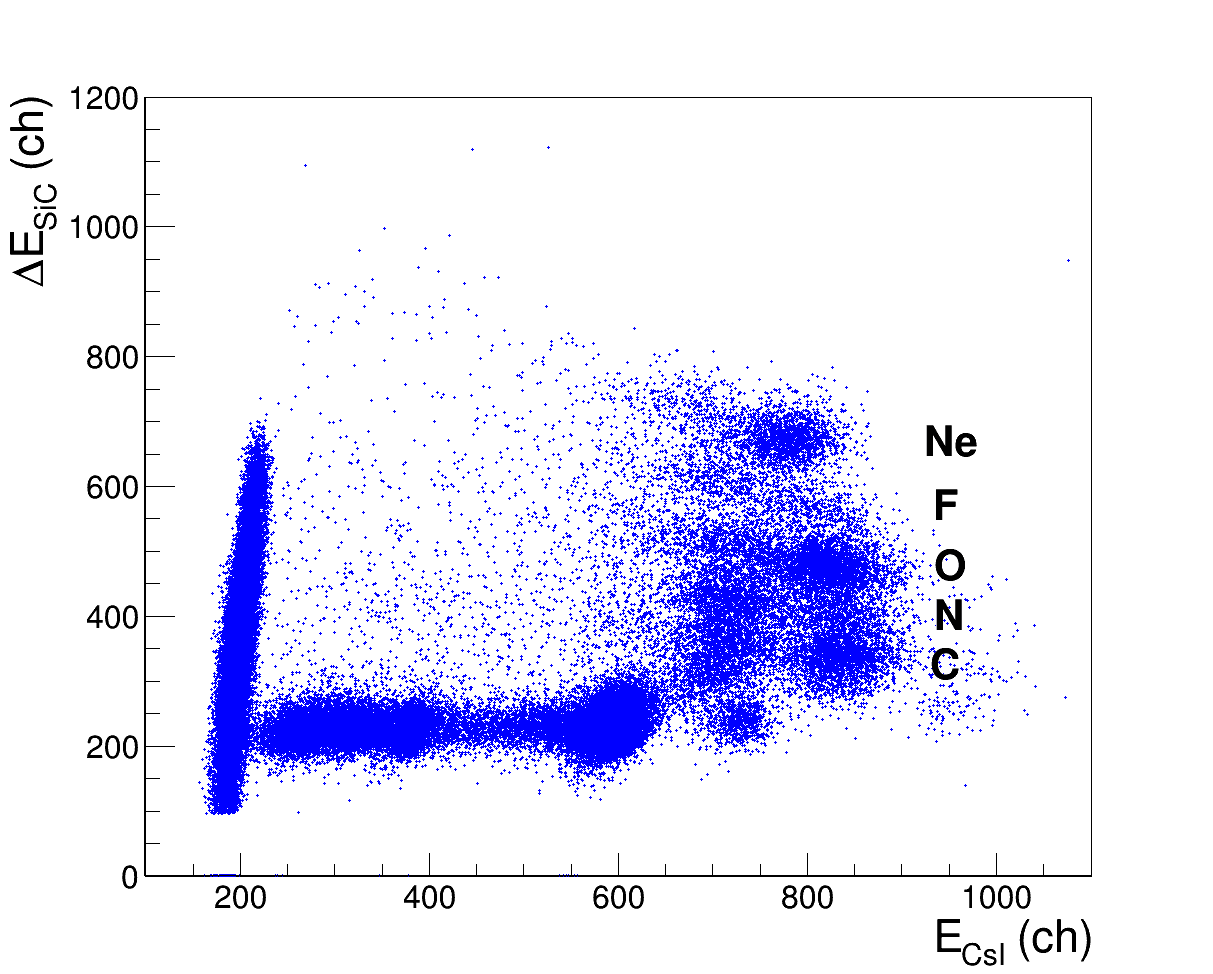
\includegraphics[width=\textwidth, keepaspectratio]{Grafici_Tesi/Test/matrice_sic_csi_vmm3a.png}
	\caption{Le correlazioni $\Delta E_{SiC} - E_{CsI}$ ottenute dal Tel~A durante il test utilizzando l'elettronica basata sul chip VMM3a.} \label{fig:sic_csi_vmm3a}
\end{figure}

\section{\iflanguage{italian}{Analisi dei dati del test beam}{Analysis of test beam data}}

Per poter confrontare i dati sperimentali con i risultati delle simulazioni è necessario che queste riproducano nel modo più fedele possibile le condizioni sperimentali; i parametri da inserire nel tool di simulazioni devono, dunque, corrispondere a quelli reali.
Alcuni fra questi parametri sono noti a priori, come ad esempio il proiettile, il bersaglio, l'energia del fascio e i campi magnetici di dipolo e quadrupolo; altri, invece, sono stati determinati attraverso un'analisi dei dati sperimentali.
Le due informazioni significative estratte da tale analisi sono il tipo di eiettile e l'energia di eccitazione del sistema eiettile-nucleo residuo.
Nei due paragrafi successivi viene descritta la procedura seguita per ricavare tali informazioni.
%Dunque, è stata svolta un'analisi dei dati raccolti durante il test per estrarre delle informazioni da inserire opportunamente nel tool di simulazioni.
%In primo luogo, è necessario stabilire quali ioni debbano costituire le particelle primarie simulate, per cui è stata svolta un'identificazione dei prodotti di reazione.
%Inoltre, poiché l'energia delle particelle primarie è un parametro di fondamentale importanza, è stata determinare l'energia con cui gli ioni incidevano sul telescopio.
%%Inoltre, dal momento che un altro parametro di fondamentale importanza riguarda l'energia di tali particelle, è stata condotta un'analisi per determinare l'energia di incidenza degli ioni sul telescopio.
%Successivamente, è stato determinato l'intervallo di energia di eccitazione del sistema eiettile-nucleo residuo.

%Ciò è stato possibile grazie alla correlazione tra posizione ed energia indotta dalla forza di Lorentz: 

\subsection{\iflanguage{italian}{Identificazione dell'\ce{^{16}O}}{Identification of \ce{^{16}O}}}

A causa della bassa statistica raccolta durante il test, è stato deciso di simulare soltanto la specie atomica più abbondante nel campione.
%, che, come si può evincere dalla Figura~, risulta essere l'Ossigeno.
La prima fase nella procedura di identificazione consiste nel determinare il numero atomico $Z$ delle particelle rivelate: tale informazione è stata ricavata dalle matrici $\Delta E_{SiC} - E_{CsI}$ in Figura~\ref{fig:sic_csi_standard}, dove si può notare che la specie atomica maggiormente presente è l'Ossigeno (O). 

Dopo avere selezionato gli ioni O è necessario distinguerne gli isotopi in numero di massa $A$; a tale scopo, si è sfruttata la correlazione, indotta dalla forza di Lorentz, tra posizione ed energia: ricordando la~\ref{eq:legge_spettrometri_approx}, è possibile notare che la misura correlata di $x_{foc}$ ed $E$ permette di separare gli ioni in base al loro rapporto $\sqrt{m}/q$, laddove $m$ e $q$ rappresentano, rispettivamente, la massa e la carica della particella.
Nel caso del telescopio, la quantità~$E$ corrisponde con buona approssimazione a $E_{CsI}$.
La matrice $x_{foc} - E_{CsI}$ è mostrata in Figura~\ref{fig:xfoc2_csi_standard}, dove è possibile osservare che gli isotopi dell'O originati dall'interazione proiettile-bersaglio sono prevalentemente \ce{^{16}O}, \ce{^{17}O} e \ce{^{18}O}.
Si sottolinea che nella correlazione $x_{foc} - E_{CsI}$ il numero di massa cresce spostandosi verso sinistra poiché, per mantenere lo stesso valore di $x_{foc}$, se la massa aumenta $E_{CsI}$ deve diminuire.
\begin{figure} [!p]
	\centering
	\includegraphics[width=\textwidth, keepaspectratio]{Grafici_Tesi2/Confronto/xfoc_ecsi.png}
	\caption{Le correlazioni $x_{foc} - E_{CsI}$ ottenute, durante il test, dalla misura in correlazione del tracciatore e del rivelatore allo CsI . La linea nera indica il taglio grafico effettuato per la selezione in numero di massa dell'\ce{^{16}O}.} \label{fig:xfoc2_csi_standard}
\end{figure}
Come si può notare dalla Figura~\ref{fig:xfoc2_csi_standard}, l'isotopo più abbondante dell'O presente nel campione è \ce{^{16}O}, la cui produzione è favorita poiché deriva da un processo di trasferimento di una particella $\alpha$ dal proiettile al bersaglio. 
La reazione scelta per la validazione della simulazione è, dunque, $^{12}\mbox{C}  ( ^{20}\mbox{Ne}, ^{16}\mbox{O} )  ^{16}\mbox{O} $.





\subsection{\iflanguage{italian}{Determinazione dell'energia di eccitazione dell'\ce{^{16}O}}{\ce{^{16}O} excitation energy evaluation}}

%Una volta identificato l'isotopo, è necessario determinare l'intervallo di energia di eccitazione esplorato dal telescopio per il sistema eiettile-nucleo residuo; infatti, in base a quanto detto nel Paragrafo~\ref{par:particelle_primarie}, fissato lo ione, il dispositivo può vedere soltanto un certo range energetico, che dipende dalla sua estensione lungo la direzione dispersiva dello spettrometro.
%Il tool è stato, quindi, utilizzato per determinare tale range: sono stati simulati diversi livelli di eccitazione fino a quando 
%Per determinare tale range è stata la correla
%Tale range è stato determinato grazie all'utilizzo del tool: sono stati, infatti, simulati diversi livelli di eccitazione dell'\ce{^{16}O} e, tramite una scelta accurata, si è fatto in modo che due di questi passassero per gli estremi 


%Una volta identificato lo ione, è necessario verificare se tale ione giunge sul telescopio in uno stato eccitato.

Uno dei parametri da inserire nel tool di simulazioni è il range di energia di eccitazione del sistema eiettile-nucleo residuo.
Nel caso in esame, tale range è stato determinato attraverso il confronto tra i dati sperimentali e i risultati di simulazioni ad hoc, a diverse energie di eccitazione, prodotte dallo stesso tool.
Tale confronto è stato realizzato nella rappresentazione che correla l'angolo orizzontale $\theta_{foc}$ della traccia al piano focale e la coordinata orizzontale $x_{foc}$ del punto di arrivo dello ione sullo stesso piano.
In Figura~\ref{fig:tefoc_xfoc} è riportata la matrice $\theta_{foc} - x_{foc}$ relativa all'\ce{^{16}O}, laddove in rosso sono rappresentati i dati raccolti con il Tel~A, in blu quelli registrati con i rivelatori al silicio del FPD e in nero i dati simulati.
Come si può notare, gli ioni di \ce{^{16}O} si trovano in uno stato altamente eccitato, che comprende un range di energia di eccitazione che va dai 32 ai 73~MeV.
Si fa, inoltre, osservare che la larghezza della striscia rossa è molto inferiore a quella delle strisce blu: ciò dipende dalla grande differenza fra la superficie del telescopio, pari a  1~cm $\times$ 1~cm, e quella dei rivelatori al silicio, ciascuna uguale a 5~cm $\times$ 7~cm.

%Tale confronto è illustrato in Figura~\ref{fig:tefoc_xfoc}, dove si pu 

%Una volta identificato lo ione, si vuole individuare il range di energia di eccitazione del sistema eiettile-nucleo residuo esplorato dal telescopio; tale energia è, infatti, collegata all'energia cinetica dell'eiettile.





%Una volta identificato lo ione, è necessario verificare se il range di energia cinetica esplorato dal telescopio per tale ione corrisponde a processi in cui il sistema eiettile-nucleo residuo sia stato eccitato.
%A tal fine, è opportuno utilizzare la correlazione tra l'angolo orizzontale $\theta_{foc}$ della traccia al piano focale e la coordinata orizzontale $x_{foc}$ del punto di arrivo dello ione sullo stesso piano.
%In Figura~\ref{fig:tefoc_xfoc} è riportata la matrice $\theta_{foc} - x_{foc}$ relativa all'\ce{^{16}O}, laddove in rosso sono rappresentati i dati raccolti con il Tel~A, mentre in blu sono indicati quelli registrati con i rivelatori al silicio di MAGNEX.



\begin{figure} [!p]
	\centering
	\includegraphics[width=\textwidth, keepaspectratio]{Grafici_Tesi2/Confronto/tefoc_xfoc_energie.png}
	\caption{Matrice $\theta_{foc} - x_{foc}$ relativa all'\ce{^{16}O}, ottenuta applicando l'AND logico dei tagli in Figura~\ref{fig:sic_csi_standard} e in Figura~\ref{fig:xfoc2_csi_standard}: in blu sono riportati i dati registrati con i rivelatori al silicio di MAGNEX, in rosso quelli raccolti con il Tel~A, in nero i risultati delle simulazioni a diverse energie di eccitazione del sistema eiettile-nucleo residuo.} \label{fig:tefoc_xfoc}
\end{figure}








\section{\iflanguage{italian}{Confronto fra i dati del test e la simulazione}{Comparison between test data and the simulation}}

%La reazione scelta per il confronto è $^{12}\mbox{C}  ( ^{20}\mbox{Ne}, ^{16}\mbox{O} )  ^{16}\mbox{O} $ a 400~MeV di energia di incidenza; inserendo i parametri rilevanti nel tool, tra cui gli ioni coinvolti, l'energia del fascio e il range di energia di eccitazione del sistema eiettile-nucleo residuo, 
%Noti tutti i parametri da inserire nel tool, è stata svolta una simulazione 



%I dati simulati sono stati elaborati dalla macro di post-processing, allo scopo di ricostruire gli spettri da comparare con i dati sperimentali.
%È bene precisare che 
Prima di effettuare il confronto tra i dati sperimentali e quelli simulati è necessario uniformare le unità di misura; infatti, mentre le distribuzioni energetiche ricavate dalla simulazione sono già espresse nell'opportuna grandezza, gli spettri sperimentali devono essere calibrati.
A tal fine, sono stati utilizzati i dati relativi allo scattering elastico del \ce{^{20}Ne} su bersaglio di \ce{^{197}Au}, per il quale i campi magnetici del dipolo e del quadrupolo sono stati opportunamente fissati facendo in modo che una parte degli ioni scatterati arrivasse sul telescopio.
È stata, dunque, svolta un'analisi per determinare l'energia cinetica con cui il \ce{^{20}Ne} incideva sul telescopio, nota la quale è stato possibile stimare il deposito energetico dello ione nel rivelatore al~SiC e nel cristallo di~CsI.
Tale stima è stata effettuata grazie a LISE++~\cite{tarasov:nimb08}, software nato per simulare la produzione di fasci di ioni attraverso meccanismi di reazioni nucleari.
In questo modo, per ciascun rivelatore era a disposizione un solo punto di corrispondenza tra la scala in canali e quella in MeV.
Di conseguenza, questa procedura ha permesso di calcolare soltanto la pendenza della retta di calibrazione, senza fissarne l'offset; quest'ultimo parametro è stato, invece, determinato sovrapponendo i centroidi delle distribuzioni sperimentale e simulata.

In Figura~\ref{fig:spettro_sic_confronto} è riportato lo spettro simulato in $\Delta E_{SiC}$, messo a confronto con quello sperimentale: come si può notare, la compatibilità delle due distribuzioni è ragguardevole; in particolare, la simulazione riproduce correttamente la larghezza dello spettro sperimentale.
La risoluzione energetica dedotta dalla simulazione sembra, quindi, rispecchiare in modo fedele quella riscontrata nel test.
%Dal momento che tale quantità gioca un ruolo cruciale nella capacità di PID del telescopio
\begin{figure} [!p]
	\centering
	\includegraphics[width=\textwidth, keepaspectratio]{Grafici_Tesi2/Confronto/sic.png}
	\caption{Spettro in $\Delta E_{SiC}$: in blu sono rappresentati i dati sperimentali, in rosso quelli simulati. Gli istogrammi sono normalizzati in area.} \label{fig:spettro_sic_confronto}
\end{figure}

In Figura~\ref{fig:spettro_csi_confronto} è illustrato il confronto tra lo spettro in $E_{CsI}$ simulato e quello sperimentale: anche in questo caso la compatibilità è significativa, sebbene, allo scopo di rappresentare meglio i dati sperimentali, la risoluzione energetica è stata aumentata dal 3 al 5\%.
Una peggiore risoluzione energetica rispetto alle assunzioni del Paragrafo~\ref{par:post-processing} può essere dovuta a diversi fatti sperimentali, come ad esempio rumore elettromagnetico o disuniformità nella raccolta di luce dello scintillatore, la quale può essere causata da un accoppiamento non ottimale con il riflettore o il fotodiodo.


\begin{figure} [!p]
	\centering
	\includegraphics[width=\textwidth, keepaspectratio]{Grafici_Tesi2/Confronto/csi.png}
	\caption{Spettro in $E_{CsI}$: in blu sono rappresentati i dati sperimentali, in rosso quelli simulati. Gli istogrammi sono normalizzati in area.} \label{fig:spettro_csi_confronto}
\end{figure}

L'accordo tra i dati sperimentali e quelli simulati è avvalorato dalla complessità della situazione trattata: in primo luogo, la reazione~\ce{^{12}C}(\ce{^{20}Ne},\ce{^{16}O})\ce{^{16}O} avviene in cinematica inversa, così che l'energia cinetica dell'eiettile risulta estremamente sensibile alla variazione dell'angolo di emissione. 
Inoltre, la presenza del substrato epitassiale davanti al volume sensibile del rivelatore al SiC genera fenomeni non-lineari nell'energia.
Infine, la bassa statistica registrata durante il test ha aumentato l'importanza delle fluttuazioni statistiche.



%\cleardoublepage
%\phantomsection
%\chapter*{\iflanguage{italian}{Conclusioni}{Conclusions}}
%\addcontentsline{toc}{chapter}{\iflanguage{italian}{Conclusioni}{Conclusions}}
%\markboth{Conclusioni}{Conclusioni}
%
%Le simulazioni computerizzate costituiscono oggi un potente strumento per studiare la risposta di un sistema di rivelazione e per analizzarne il comportamento al variare delle sue caratteristiche.
Le simulazioni computerizzate costituiscono oggi un potente strumento per studiare la risposta di un sistema di rivelazione e per dedurre utili informazioni sulle specifiche tecniche ottimali.
Nell'ambito del progetto NUMEN è stata realizzata una simulazione basata sulla piattaforma \geant{}, allo scopo di valutare le prestazioni di un sistema per la rivelazione e l'identificazione di ioni pesanti ad alto rate, costituito da un muro di telescopi $\Delta E - E_{resid}$ a stato solido.
Tale simulazione ha permesso di verificare che una soluzione basata sulla tecnologia SiC-CsI può soddisfare le performance necessarie per gli obiettivi del progetto, garantendo una buona separazione degli ioni di interesse per NUMEN lungo tutto il range energetico preso in considerazione.
Dal momento che il progetto intende studiare le reazioni di doppio scambio di carica (Double Charge Exchange, DCE), le quali sono caratterizzate da sezioni d'urto estremamente basse, un importante aspetto di questo lavoro è consistito nello stimare la percentuale di eventi identificati in modo erroneo: in tutti i casi esaminati, tale quantità è risultata inferiore ai limiti imposti sulla perdita di segnali corretti e sulla contaminazione originata dal fondo.


È stato, inoltre, osservato che, ai fini della Particle IDentification (PID), la correlazione $\Delta E - E_{resid}$ produce prestazioni analoghe a quelle della correlazione $\Delta E - E_{tot}$, rendendo, dunque, non necessaria la calibrazione dei due stadi del telescopio.

Diversi studi sono stati condotti variando le dimensioni trasversali dei rivelatori, dai quali è emerso che la percentuale di eventi affetti da raccolta di carica incompleta, principale fonte di errore nell'identificazione, diminuisce all'aumentare della superficie sensibile. 
Tuttavia, in condizioni di alti flussi di particelle incidenti, come quelli previsti per NUMEN, un fenomeno da tenere in considerazione per la scelta delle dimensioni dei rivelatori è il pile-up.
È stato, dunque, effettuato un calcolo analitico allo scopo di studiare l'andamento della probabilità di pile-up al variare della superficie del rivelatore, dal quale è risultato che tale quantità aumenta velocemente al crescere delle dimensioni trasversali.
Di conseguenza, dal compromesso tra le due esigenze, si è dedotto che la configurazione ottimale per gli scopi del progetto prevede l'utilizzo di telescopi da $1.5 \times 1.5$~cm\ap{2}.


L'analisi dell'influenza degli effetti di bordo del rivelatore al SiC sulle capacità di PID ha consentito di sostenere che la percentuale di eventi degradati cresce all'aumentare della lunghezza della regione di transizione, ma resta comunque entro i limiti fissati.
Dunque, anche nel caso in cui tali rivelatori dovessero avere una regione parzialmente attiva con una lunghezza maggiore dei 50~$\mu$m assunti come valore di riferimento, le prestazioni di identificazione non dovrebbero subire sostanziali peggioramenti.



Lo studio sul substrato epitassiale del rivelatore al SiC ha fatto emergere che la riduzione dello spessore dai 350 ai 10~$\mu$m provoca un aumento della percentuale di eventi degradati, risultando in un peggioramento delle performance di PID.
Dunque, dal punto di vista dell'identificazione, l'ablazione LASER del substrato si configura come un'operazione ingiustificata, nonché potenzialmente dannosa in termini di resa di produzione dei dispositivi.


Un aspetto fondamentale di questo lavoro è consistito nella validazione della simulazione Monte Carlo attraverso il confronto con i dati sperimentali raccolti in occasione del test beam svolto ad Aprile 2019.
Tale test aveva lo scopo di studiare le prestazioni del primo prototipo di telescopio SiC-CsI per NUMEN, utilizzando sia l'elettronica tradizionale di MAGNEX sia il primo esemplare di elettronica di front-end VMM3a realizzato per il progetto.
I dati sperimentali sono stati analizzati allo scopo di ricostruire i parametri essenziali da introdurre nella simulazione, come ad esempio il numero atomico e il numero di massa della particella primaria e il range energetico.
È stata, dunque, svolta un'identificazione utilizzando le correlazioni $\Delta E_{SiC} -E_{CsI}$ e $x_{foc} -E_{CsI}$, allo scopo di selezionare lo ione più abbondante nel campione, risultato essere l'\ce{^{16}O}.
Grazie alla tecnica basata sulla deflessione causata dalla forza di Lorentz è stato possibile ricavare la distribuzione in energia cinetica di tale ione, la quale è stata riprodotta nella simulazione.
Gli spettri energetici registrati dal rivelatore al SiC e dallo scintillatore allo CsI sono stati messi a confronti con i rispettivi spettri simulati: in entrambi i casi la compatibilità è significativa, in particolar modo per quanto riguarda il rivelatore al SiC.
Alla luce di questo accordo è possibile affermare che la simulazione riesce a riprodurre bene la realtà sperimentale, convalidando i risultati ottenuti nel corso di questo lavoro.





%Dal momento che, per raggiungere i propri obiettivi, il progetto deve spingersi al limite delle attuali possibilità nel campo degli esperimenti con fasci di ioni pesanti ad elevata intensità, è essenziale la ricerca e sviluppo di tecnologie di frontiera.
%In tale prospettiva si inquadra 
%Le stringenti esigenze di resistenza alle radiazioni hanno guidato verso la scelta di un primo stadio 
%%L'introduzione di tale sistema rientra in un più grande scenario che prevede una profonda opera di ristrutturazione del Ciclotrone Superconduttore K800 e dello spettrometro magnetico MAGNEX.
%Lo scopo di tale upgrade consiste nell'aum
%alla fine della quale sarà possibile ottenere fasci di ioni pesanti ad elevata intensità.
%%Tale upgrade ha l'obiettivo di aumentare l'intensità dei fasci di ioni pesanti attualmente disponibili di almeno due ordini di grandezza, al fine di poter avviare una campagna di studi sistematica di tutti gli isotopi coinvolti nel doppio decadimento beta senza neutrini (\doppiobeta).
%Tale condizione richiede un'intensa attività di ricerca e sviluppo in diversi campi della tecnologia coinvolta negli esperimenti 
%%Il raggiungimento di intensità così elevate rende necessaria un'intensa attività di ricerca e sviluppo in diversi campi della tecnologia coinvolta negli esperimenti di collisione di ioni pesanti; in particolare, innumerevoli studi sono stati dedicati all'analisi delle proprietà di resistenza alle radiazioni dei materiali e dei sistemi da utilizzare.
%in particolare, dal momento che la resistenza alle radiazioni è un requisito imprescindibile per la scelta dei materiali e dei sistemi da utilizzare, innumerevoli studi sono stati condotti 
%%Dal momento che i rivelatori al silicio non sono in grado di tollerare le intensità previste, il primo stadio del telescopio sarà basato su un rivelatore sottile (100~$\mu$m) al carburo di silicio (SiC), materiale che, grazie alle sue caratteristiche, ha attirato notevole interesse da parte della comunità scientifica.
%%Il rivelatore di stop del telescopio sarà, invece, costituito da un cristallo allo ioduro di cesio (CsI) dello spessore di 1~cm.
%Un'importante linea di ricerca è stata, dunque, avviata sulla realizzazione e caratterizzazione di rivelatori sottili basati su tale materiale.
%%Tuttavia, la resistenza alle radiazioni non è l'unico requisito che il sistema di identificazione deve possedere; infatti, esso deve in primo luogo consentire di discriminare in modo efficace gli ioni nella regione di interesse per NUMEN, costituita principalmente da Ossigeno, Fluoro e Neon.
%%Inoltre, esso deve possedere una risoluzione energetica tale da preservare le prestazioni dell'attuale apparato riguardo all'identificazione in numero atomico e numero di massa dei prodotti di reazione.










%\lipsum[20]


\cleardoublepage
\phantomsection
\addcontentsline{toc}{chapter}{\iflanguage{italian}{Bibliografia}{Bibliography}}
\bibliographystyle{mprsty}
\bibliography{biblio}


%\cleardoublepage
%\phantomsection
%\chapter*{\iflanguage{italian}{Ringraziamenti}{Acknowledgements}}
%\addcontentsline{toc}{chapter}{\iflanguage{italian}{Ringraziamenti}{Acknowledgements}}

%\lipsum[20]

\end{document}




